%--------------------------------------------------------------------------
% This LaTeX document was developed for my GmE300 master's thesis submitted
% as a requirement under the Master of Geomatics Engineering, Major in 
% Remote Sensing at the Department of Geodetic Engineering, University of 
% the Philippines Diliman.
%
% The LaTeX template follows the thesis manuscript template prescribed by
% the National Graduate School of Engineering, which may also be used as 
% template by graduate students for creating thesis manuscripts from other 
% departments.
% 
% This template was based on the original template written by M. Imran
% (18 Jun 2001), and subsequently updated by Ian Craig (20 Oct 2014) based 
% on the Mechanical Engineering Thesis Guidelines, the University of New 
% South Wales, Australia. 
%
% Revision by:		Jose Don T. De Alban
% Date revised:		30 Jun 2017	
% License: 
% 
%--------------------------------------------------------------------------
%
% This main 'GmE300_Thesis.tex' file controls the whole document. It has 
% three functions:
%   1. Include and configure any packages used in the document
%   2. Define page numbering, structure, and bibliography
%   3. Import/Include all other files
%
%--------------------------------------------------------------------------

\documentclass[thesis]{GmE300_Thesis}

%--------------------------------------------------------------------------
% Load Packages
%--------------------------------------------------------------------------
\usepackage{algorithm}
\usepackage{algpseudocode} % Display algorithms nicely. http://goo.gl/6Z93aV
\usepackage{amsmath}
\usepackage{amssymb}
\usepackage{array}
\usepackage{booktabs} % From http://goo.gl/2ezu9p to make tables look nicer.
\usepackage{caption}
%\usepackage{cite}
\usepackage{color}
\usepackage{ctable}
\usepackage[draft]{listofsymbols} % Add list of symbols.
\usepackage{epic}
\usepackage{epsfig}
\usepackage{epstopdf}
\usepackage{fancyhdr}
\usepackage{fmtcount}
\usepackage{graphics}
\usepackage{graphicx}
\usepackage{hyperref}
\usepackage{indentfirst} % To indent first line of paragraph
\usepackage{latexsym}
\usepackage{longtable}
\usepackage{ltablex}
\usepackage{mathtext}
\usepackage{mdwlist} % To reduce list vertical spacing. http://goo.gl/nyLux
\usepackage{microtype} % To improve line filling
\usepackage{multirow}
%\usepackage{natbib}
\usepackage{pdflscape} % Rotate display of landscape pages in PDFs http://goo.gl/wbg4fy
\usepackage{printlen} % Print variables. http://goo.gl/3ZdAPV
\usepackage{setspace}
\usepackage{subcaption} % Replaces subfig and subfigure.
\usepackage{tabularx}
\usepackage{theorem}
\usepackage[toc,page]{appendix}
\usepackage{usnomencl} % For making a glossary of nomenclature.
\usepackage{url}
\urlstyle{rm}

%\uselengthunit{in} % See above
%\printlength{\textwidth} % See above
%\the\textwidth   % \textwidth = 426.79134 pt = 149.99823 mm = 5.90666 in. An alternative method of printing variables.
% @300dpi --> 1771 px.
% For adding Latex Section symbols to the actual headings:
%\usepackage{titlesec}. 
%\titleformat{\section}{\normalfont\Large\bfseries}{\S\thesection}{1em}{}
% For cyrillic font (naiive i)
%\usepackage[OT2,OT1]{fontenc} 


%--------------------------------------------------------------------------
% Setup
%--------------------------------------------------------------------------

% Bibliography File Path
\bibliography{../MSc Thesis/references/bibliography}

% Inputs
%--------------------------------------------------------------------------
% This is the 'format.tex' file required for the 'GmE300_Thesis.cls' class
% file. It defines the style and formatting of the document, which can be 
% configured. The remaining style is defined by 'GmE300_Thesis.cls' file.
%--------------------------------------------------------------------------

% Note: Place packages to use here and 'fancyhdr' is required.

%\hlopts{bwidth=0}
%\hlopts[url]{colormodel=named,color=BlueViolet}
%\hypersetup{linkcolor=cyan,citecolor=cyan,urlcolor=cyan}


%--------------------------------------------------------------------------
% Fancy Header
%--------------------------------------------------------------------------

% Note: Remove '\bfseries\today' below for final copy

%\pagestyle{fancy}
%\renewcommand{\chaptermark}[1]{\markright{\chaptername\ \thechapter.\ #1}}
%\renewcommand{\sectionmark}[1]{\markright{\thesection.\ #1}{}}
%\lhead[\fancyplain{}{}]%
%      {\fancyplain{}{\bfseries\rightmark}}
%\chead[\fancyplain{}{}]%
%      {\fancyplain{}{}}
%\rhead[\fancyplain{}{}]%
%      {\fancyplain{}{\bfseries\thepage}}
%\lfoot[\fancyplain{}{}]%
%      {\fancyplain{}{}}
%\cfoot[\fancyplain{}{}]%
%      {\fancyplain{}{}}
%\rfoot[\fancyplain{}{}]%
%      {\fancyplain{}{\bfseries\today}}


%--------------------------------------------------------------------------
% Set space between main text and the start of the footnote
%--------------------------------------------------------------------------

%\addtolength{\skip\footins}{5mm}


%--------------------------------------------------------------------------
% Define new counter to be used for equation numbers
%--------------------------------------------------------------------------

\newcounter{ind}
\def\eqlabon{
\setcounter{ind}{\value{equation}}\addtocounter{ind}{1}
\setcounter{equation}{0}
\renewcommand{\theequation}{\arabic{chapter}%
         .\arabic{section}.\arabic{ind}\alph{equation}}}
\def\eqlaboff{
\renewcommand{\theequation}{\arabic{chapter}%
         .\arabic{section}.\arabic{equation}}
\setcounter{equation}{\value{ind}}}


%--------------------------------------------------------------------------
% Define new theorem to be used
%--------------------------------------------------------------------------

{\theorembodyfont{\rmfamily}\newtheorem{Pro}{{\textbf Proposition}}[section]}
{\theorembodyfont{\rmfamily}\newtheorem{The}{{\textbf Theorem}}[section]}
{\theorembodyfont{\rmfamily}\newtheorem{Def}[The]{{\textbf Definition}}}
{\theorembodyfont{\rmfamily}\newtheorem{Cor}[The]{{\textbf Corollary}}}
{\theorembodyfont{\rmfamily}\newtheorem{Lem}[The]{{\textbf Lemma}}}
{\theorembodyfont{\rmfamily}\newtheorem{Exp}{{\textbf Example}}[section]}
\def\remark{\textbf{Remark}:}
\def\remarks{\textbf{Remarks}:}
\def\bproof{\textbf{Proof}: }
\def\eproof{\hfill$\Box$}


%--------------------------------------------------------------------------
% Bold fonts in math mode
%--------------------------------------------------------------------------

\def\bv#1{\mbox{\boldmath$#1$}}


%--------------------------------------------------------------------------
% New symbols not defined in LaTeX
%--------------------------------------------------------------------------

% The Mean INTegral
% to be used in displaystyle
	\def\mint{\textstyle\mints\displaystyle}
% to be used in textstyle
	\def\mints{\int\!\!\!\!\!\!{\rm-}\ }

% The Mean SUM
% to be used in displaystyle
	\def\msum{\textstyle\msums\displaystyle}
% to be used in textstyle
	\def\msums{\sum\!\!\!\!\!\!\!{\rm-}\ }
	

%--------------------------------------------------------------------------
% Define shortcuts here
%--------------------------------------------------------------------------

\def\poincare{Poincar\'e }
\def\holder{H\"older }


%--------------------------------------------------------------------------
% Small font captions
%--------------------------------------------------------------------------

% Different font in captions
\newcommand{\captionfonts}{\small}

\makeatletter % Allow the use of @ in command names
\long\def\@makecaption#1#2{%
  \vskip\abovecaptionskip
  \sbox\@tempboxa{{\captionfonts #1: #2}}%
  \ifdim \wd\@tempboxa >\hsize
    {\captionfonts #1: #2\par}
  \else
    \hbox to\hsize{\hfil\box\@tempboxa\hfil}%
  \fi
  \vskip\belowcaptionskip}
\makeatother % Cancel the effect of \makeatletter

\renewcommand{\figurename}{Fig.}
 % format.tex
%--------------------------------------------------------------------------
% Document Variables
%--------------------------------------------------------------------------

\newcommand{\thesistitle}[0]{\textrm{Evaluation of multi-year ALOS/PALSAR mosaic data for mapping and monitoring of forest cover types in the Philippines}}
\newcommand{\authorname}[0]{\textrm{Jose Don T De Alban}}
\newcommand{\thesismonthyear}[0]{\textrm{January 2017}}
\newcommand{\advisername}[0]{\textrm{Enrico C Paringit, Dr Eng}}


%--------------------------------------------------------------------------
% Figures
%--------------------------------------------------------------------------

\newcommand{\executeiffilenewer}[3]{%
\ifnum\pdfstrcmp{\pdffilemoddate{#1}}%
{\pdffilemoddate{#2}}>0%
{\immediate\write18{#3}}\fi%
}
\newcommand{\includesvg}[1]{%
\executeiffilenewer{#1.svg}{#1.pdf}%
{inkscape -z -D --file=#1.svg %
--export-pdf=#1.pdf --export-dpi=600 --export-latex}%
\input{#1.pdf_tex}%
}

\newcommand{\vectornorm}[1]{\left|\left|#1\right|\right|} % commands.tex
\graphicspath{{./images/}} % images directory

\begin{document}
	
	%--------------------------------------------------------------------------
% List of Symbols
%--------------------------------------------------------------------------

\opensymdef
% Note that \mathcal is not permitted in math mode in the description.
% See: 
% 	\url{http://www.latex-community.org/forum/viewtopic.php?f=46&t=15307}
% 	\url{http://www.latex-community.org/forum/viewtopic.php?f=4&t=2096}
% Sort out notation for vectors, matrices, and scalars!!
% Chapter 3:
    \newsym[Set of sample points]{samplepts}{\Omega}
    \newsym[Belief state estimate]{bse}{\hat{X}}
\closesymdef  % symbolslist.tex

	% Header Pages
	%--------------------------------------------------------------------------
% Cover Page
%--------------------------------------------------------------------------

% The cover page is based on the National Graduate School of Engineering, University of the Philippines Diliman thesis guidelines

\pagenumbering{roman}
\setcounter{page}{1}
%\setcounter{secnumdepth}{3}

\newpage
\thispagestyle{empty}
\begin{center}

	% Insert university logo
	\begin{figure}
	\centering
	
\includegraphics{cov_upd-logo.png}
	\label{fig: cover-uplogo}
	\end{figure}

  	% Insert text
  	{UNIVERSITY OF THE PHILIPPINES\\[0.5cm]
	 Master of Science in Geomatics Engineering}
  	 \vspace*{1cm}
  
  	{\textbf \authorname}
  	 \vspace*{0.2cm}
  
  	\begin{singlespace}
  		{\thesistitle}
  	\end{singlespace}  
  
  	\vspace*{0.5cm}

	{Thesis Adviser:}\\[0.5cm]
	 \begin{singlespace}
  	 	\textbf \advisername\\
  	 	{Department of Geodetic Engineering\\
  	 	University of the Philippines Diliman}
  	 \end{singlespace}
  	 \vspace*{1cm}

  	{Date of Submission:\\ 
  	 \thesismonthyear}
  	 \vspace*{1cm}
  	
  	{Thesis Classification:\\ 
  	 \textbf{F}\\
  	 This thesis is available to the public.}
  	 \vspace*{1cm}  

\end{center}


%--------------------------------------------------------------------------
% Approval Page
%--------------------------------------------------------------------------
\newpage
\thispagestyle{empty}

\begin{singlespace}
This thesis entitled, \textbf{\MakeUppercase \thesistitle}, prepared and submitted by \textbf{\MakeUppercase \authorname}, in partial fulfillment of the requirements for the degree of \textbf{GEOMATICS ENGINEERING}, major in \textbf{REMOTE SENSING} is hereby accepted.
\end{singlespace}

\vspace*{1cm}

\begin{singlespace}
	{\noindent\hspace*{7cm}\textbf{\MakeUppercase \advisername}}\\
	{\hspace*{9.2cm}Thesis Adviser}
\end{singlespace}

\vspace*{6cm}

\begin{singlespace}
Accepted as partial fulfillment of the requirements for the degree of \textbf{GEOMATICS ENGINEERING}, major in \textbf{REMOTE SENSING}.
\end{singlespace}

\vspace*{1cm}

\begin{singlespace}
	{\noindent\hspace*{7.4cm}\textbf{\MakeUppercase {Dr Rizalinda L De Leon}}}\\
	{\hspace*{10.1cm}Dean}
\end{singlespace}


%--------------------------------------------------------------------------
% Acknowledgement
%--------------------------------------------------------------------------
\newpage
\thispagestyle{empty}
\chapter*{Acknowledgement}

%--------------------------------------------------------------------------
% Acknowledgements
%--------------------------------------------------------------------------

This thesis is the product of perseverance and hard work from my long, meandering journey in pursuit of achieving a master’s degree, and of wanting to do research that not only aligned with my own interests in applying remote sensing for forest conservation and management, but also of contributing an academic piece of work with a practical purpose. It is my hope that this thesis is found in the hands of individuals who by reading, studying, critiquing, and improving it find value in this work\textemdash all to further contribute to the greater body of knowledge\textemdash rather than just ending up unread in shelves, gathering dust.

Completing this master’s thesis would not have been possible without the support and encouragement of family, friends, and colleagues, especially when my commitment to family and professional work took precedence over finishing my postgraduate studies. I am so grateful to all of you.

To Dr Enrico Paringit, my thesis adviser and professor, for sharing his knowledge and providing guidance in doing my thesis, and for his patience, understanding, persistence, and encouragement all throughout my master’s studies.

To Dr Rijaldia Santos and Engr Ma Rosario Concepcion Ang, both of whom were my former professors during my undergraduate and masters studies, respectively. Thank you for agreeing to be my thesis panel members and providing very helpful comments during my thesis viva and for improving the manuscript.

To this extraordinary group of friends, colleagues, research group mates wherein our professional, academic, and even personal lives have been intertwined: Angelica Kristina Monzon, Rizza Karen Veridiano, Margie Parinas, Sheryl Rose Reyes, Roven Tumaneng, Ray Neil Lorca, Raul Magabo, and Francisco Tavora Jr\textemdash this journey was all the more worthwhile because we were all in the thick of things together.

To my former professors, including Dr Ariel Blanco, Dr Rhodora Gonzalez, and Dr Ma Cecilia Rubio-Paringit, who kept encouraging me to finish my thesis at every opportunity that I meet them. This also goes for my boss at my new research work at the National University of Singapore, Dr Edward Webb\textemdash thanks for keeping me on my toes.

To close friends and colleagues: Edmund Leo Rico, Ronald Allan Altamirano, and Dr Neil Aldrin Mallari\textemdash thank you all for those long discussions, brainstorming sessions, and exchange of ideas of the things that make us look forward to waking up in the morning.

I am also grateful to Mari Trix Estomata, Nimol Vameourn, Christian Supsup, Dennis Tacmo, Dr Edwino Fernando, and Ms Rhudelene Serrano who have all supported me in small ways but nevertheless added up to help me put my thesis together.

This work has been undertaken within the framework of the Kyoto \& Carbon Initiative led by Japan Aerospace Exploration Agency. The ALOS/PALSAR data used in this study have been provided by the JAXA Earth Observation Research Center.

I dedicate this academic work to Rina, my wife and best friend, and my twin daughters, Dahon Luntian and Ulap Amihan\textemdash you are all my inspiration.

And to God for whom all of this was meant for his greater honor and glory.

%--------------------------------------------------------------------------
% Abstract
%--------------------------------------------------------------------------
\newpage
\thispagestyle{empty}
\chapter*{Abstract}

%--------------------------------------------------------------------------
% Abstract
%--------------------------------------------------------------------------

Forests are important ecosystems that provide a broad range of goods and services, including social and economic benefits in the long term. To sustainably manage forest resources, remote sensing technologies are being employed as an accurate and cost-effective approach for mapping and monitoring forest conditions. In the Philippines, spaceborne remote sensing technology was similarly used in the past for forest resources assessment and management. The mapping efforts, however, were fraught with limitations in terms of temporal consistency and availability of optical data; inconsistent forest classification systems used; and replicability of approaches. This study evaluated the suitability of ALOS/PALSAR mosaic data for mapping and monitoring of forest cover types in the Philippines by assessing temporal consistency, forest classification hierarchy, and classification accuracy. Digital image processing approaches were used including object-based segmentation, extraction of texture features, hierarchical clustering, and decision tree classification. A combination of feature attributes including polarimetric, topographic, and texture information were assessed. Results showed that the ALOS/PALSAR mosaics were temporally consistent within a single acquisition year and across multiple acquisition years, making it a suitable data product for mapping and monitoring forests. Combining polarimetric, topographic, and texture attributes yielded better classification accuracies compared to using polarimetric SAR data alone, although the addition of ancillary feature attributes marginally decreased temporal consistency of the input data. Employing a decision tree classification approach identified the most relevant image layers and feature attributes for classifying different classes. Hierarchical multi-level classification provided a consistent approach for quantifying the degree of accuracy in discriminating different forest cover types. However, even with the best combination of feature attributes used in study, low classification accuracies were obtained in discriminating forest cover types. Although compared to heuristic methods, using a hierarchical clustering analysis to find natural groupings of forest types in the data yielded better classification accuracies. ALOS/PALSAR was not suitable for discriminating forest types based on the FAO Global Forest Resource Assessment classification scheme, and exploring other classification schemes is recommended.


%--------------------------------------------------------------------------
% Table of Contents
%--------------------------------------------------------------------------

% Note: Comment out as necessary

%\setcounter{secnumdepth}{3}
\tableofcontents 
\clearpage


%--------------------------------------------------------------------------
% Acronyms
%--------------------------------------------------------------------------

% Note: Nomenclature superceded by \listofsymbols package.
\newpage
\thispagestyle{empty}
\chapter*{Acronyms}

%--------------------------------------------------------------------------
% Acronyms
%--------------------------------------------------------------------------

\begin{Nomencl}[3cm]
	\item[ALOS] 	Advanced Land Observing Satellite
	\item[AU] 		Approximately Unbiased
	\item[AVHRR] 	Advanced Very High Resolution Radiometer
	\item[CART] 	Classification and Regression Trees
	\item[DEM] 		Digital Elevation Model
	\item[ERS] 		European Resource Satellite
	\item[FAO] 		Food and Agriculture Organisation of the United Nations
	\item[FCCS] 	Forest Cover Classification System
	\item[FMB] 		Forest Management Bureau
	\item[GEOBIA] 	Geographic Object-Based Image Analysis
	\item[GFRA] 	Global Forest Resources Assessment
	\item[GIS] 		Geographic Information System
	\item[GLCM] 	Grey Level Co-occurrence Matrix
	\item[HH] 		Horizontal transmit - Horizontal receive
	\item[HV] 		Horizontal transmit - Vertical receive
	\item[IQR] 		Inter-Quartile Range
	\item[JAXA] 	Japan Aerospace Exploration Agency
	\item[JERS] 	Japan Earth Resources Satellite
	\item[LCCS] 	Land Cover Classification System
	\item[NAMRIA] 	National Mapping and Resource Information Authority
	\item[NFA] 		National Forest Assessment
	\item[OBIA] 	Object-Based Image Analysis
	\item[PALSAR] 	Phased Array type L-band Synthetic Aperture Radar
	\item[REDD+] 	Reducing Emissions from Deforestation and Forest Degradation - Plus
	\item[ROI] 		Region of Interest
	\item[SAR] 		Synthetic Aperture Radar
	\item[SIR] 		Shuttle Imaging Radar
	\item[SRTM] 	Shuttle Radar Topography Mission
	\item[SSC] 		Swedish Space Corporation
	\item[UN] 		United Nations
	\item[VH] 		Vertical transmit - Horizontal receive
	\item[VV] 		Vertical transmit - Vertical receive
\end{Nomencl}
\clearpage



%--------------------------------------------------------------------------
% Lists
%--------------------------------------------------------------------------

% Note: Comment out as necessary

%\setcounter{secnumdepth}{3}
\listoftables
\listoffigures
%\listofsymbols
%\nomencl
\clearpage


%--------------------------------------------------------------------------
% Measurement Units
%--------------------------------------------------------------------------

% Note: Nomenclature superceded by \listofsymbols package.
\newpage
\thispagestyle{empty}
\chapter*{Measurement Units}

%--------------------------------------------------------------------------
% Measurement Units
%--------------------------------------------------------------------------

\begin{Nomencl}[3cm]
	\item[B] 		billion
	\item[dB] 		decibel
	\item[ha]	 	hectare
	\item[km] 		kilometer
	\item[m] 		meter
	\item[M] 		million
	\item[yr] 		year
\end{Nomencl}
\clearpage




	% Setup Contents
	\pagenumbering{arabic}
	\setcounter{page}{1}
	\setcounter{chapter}{0}
	\setcounter{equation}{0}

	% Chapters
	%--------------------------------------------------------------------------
% Introduction
%--------------------------------------------------------------------------

\chapter{Introduction}
\label{cha: introduction}

\section{Background}
\label{sec: intro-background}

Forests are complex, functional systems of interacting and interdependent biological, physical, and chemical components, which creates unique combinations of climate, soil, plant and animal species that result in many different forest types around the world (\cite{blanco_forest_2012}). These ecosystems harbor the vast majority of biological species on Earth (\cite{pan_structure_2013}), account for 80\% of the Earth’s total plant biomass (\cite{kindermann_global_2008}), and store more carbon in biomass and soils than is contained in the atmosphere (\cite{pan_large_2011}). Forests not only play an important role in supporting and maintaining ecological systems and cycles, but also provide a broad range of goods and services to humanity, including social and economic benefits in the long term (\cite{fao_global_2015}). Among the valuable ecosystem goods and services provided by forests are food, fibre, timber, medicine, clean water, aesthetic and spiritual values, climate regulation, a repository of carbon storage, and mitigation of natural hazards such as floods (\cite{pimentel_value_1997}; \cite{pearce_economic_2001}; \cite{blanco_forest_2012}; \cite{pan_structure_2013}; \cite{chazdon_when_2016}).

Nearly 1.6 billion people comprising more than 25\% of the world’s population depend on forest resources for their livelihoods (FAO, 2015a), and another estimated 410 million people are highly dependent on forests for their subsistence and income (Munang et al., 2011). Recent estimates of the global economic values of terrestrial forest ecosystems increased from US\$ 2,769/ha/yr in 1997 to US\$ 5,682/ha/yr in 2011 for tropical forests, and from US\$ 417/ha/yr in 1997 to US\$ 3,137/ha/yr in 2011 for temperate/boreal forests (standardised in terms of 2007 US\$ values; Costanza et al. 2014). The estimates of the economic value of mangrove forests were even higher at US\$ 13,786/ha/yr in 1997 to US\$ 193,843/ha/yr in 2011, which were mainly due to new studies of the value of mangroves in terms of storm protection, erosion prevention, and waste treatment (Costanza et al., 2014).

Despite their renowned importance, however, forests have declined at a staggering rate around the world. Achard et al. (2014) showed that 8.0 M ha/yr of tropical forests were lost between 1990 to 2000, which decreased to 7.6 M ha/yr between 2000 to 2010. Another study by Mayaux et al. (2005) further estimated the annual rates of forest loss in the 1990s for different forest types, particularly 5.8 M ha/yr of humid tropical rainforests, 2.2 M ha/yr of tropical moist deciduous forests, and 0.7 M ha/yr of tropical dry forests. For the period between 2000 to 2012, Hansen et al. (2013) mapped global forest cover change and estimated that a total of 230 M ha of forest were lost due to disturbance while 80 M ha of new forests were established, from which 20 M ha of land experienced both forest loss and forest gain.

Tropical deforestation was mainly driven by agricultural expansion, commercial wood extraction, and infrastructure extension, which were prominently underpinned by economic, political, and institutional factors (Geist \& Lambin, 2002). Agricultural expansion was the main driver of forest cover loss across the tropics between the period of 1980 to 2000, wherein more than 55\% of new agricultural land replaced intact forests and another 28\% came from disturbed forests (Gibbs et al., 2010).

As of 2015, forests occupy 30.6\% of the Earth’s total land area (FAO, 2015b). But although the world's forests decreased from 4.128 B ha in 1990 to 3.999 B ha in 2015 (Keenan et al., 2015), the Food and Agriculture Organisation (FAO) reported that this 25-year period has seen positive results overall, such as in the rate of global net forest loss being cut by over 50\% (i.e., decreased to 0.08\% annually since 2010 being half the rate in the 1990s; Sloan \& Sayer, 2015); the higher attention given to sustainable forest management worldwide (MacDicken et al., 2015); that forests are meeting increasing demand for a variety of forest products and services (Payn et al., 2015); and larger areas being designated for biodiversity conservation (Morales-Hidalgo et al., 2015).

Sustainable forest management is key to ensuring that the ever-increasing demands of a growing human population are met while maintaining ecological functions of healthy forest ecosystems (MacDicken et al., 2015). Forest resources assessment forms an essential part of sustainable forest management, and determining the nature and distribution of land cover is the first step in any forest resources assessment (van der Sanden \& Hoekman, 1999). Gathering better information to monitor and analyse the status and trends on forest resources can further improve forest management (Siry et al., 2005). To this end, accurate estimates of the extent of forests and forest types are indispensable for understanding forest ecosystems and their sustainable use (Foody, 2003), of which remote sensing techniques have been reliably employed over the past several decades as an accurate, systematic, and cost-effective approach for mapping and monitoring forest conditions and changes across a range of scales (Myers, 1988; Franklin, 2001; Dahdouh-Guebas, 2002; Boyd \& Danson, 2005). Combining remote sensing with field observations provides a comprehensive monitoring approach in support of sustainable forest management at a range of scales (Keenan et al., 2015).

\section{Remote sensing of Philippine forests}
\label{sec: intro-rs-phil-forests}

In the Philippines, a nation-archipelago located between the equator and the Tropic of Cancer in Southeast Asia, forests harbor extremely high floral and faunal diversity, and at the same time also serve as home to upland communities that are highly dependent on forest resources (Lasco \& Pulhin, 2000). Studies have cited estimates of the extent of forest cover to be \url{~}90\% of the 30 M ha total land area of the Philippine islands before the Spanish colonisation in 1521, down to \url{~}70\% at the transition of colonial regimes between Spain and America by 1900s, and further reduced to \url{~}60\% during the Japanese occupation of the Philippines from 1942 to 1945 (Kummer, 1992a; Liu et al., 1993; Bankoff, 2007). During the 20th century, the average deforestation rate in the Philippines was estimated to be 148,000 ha/yr (Lasco \& Pulhin, 2000). Recent official forestry statistics in 2015 reported a decline in forest cover from 7.17 M ha in 2003 to 6.84 M ha in 2010 (FMB, 2015). Timber harvesting and agricultural expansion during the Spanish colonisation, followed by rapid and extensive commercial logging in the 20th century were recognised as the main drivers of historical forest loss in the Philippines (Eder, 1990; Kummer, 1992a; Chokkalingam et al., 2006; Bankoff, 2007).\\

\begin{spacing}{1.0}
\begin{longtable}[h!]{ p{1cm} p{5.4cm} p{2.2cm} p{1.9cm} p{2.5cm} }

    \caption[National forest surveys in the Philippines using remotely sensed data.]{National forest surveys in the Philippines using remotely sensed data (adopted from Kummer, 1992b).}
    \label{tab: intro-table1.1}\\
    
    	\toprule
    	Year & Source & Forest & Data & Method of\\ 
		{} & {} & Cover (\%) & Source & Interpretation\\ 
    	\midrule
    	\endhead
    	
		1973 & Lachowski et al. (1979) & 38.0 & Landsat & Digital\\
		1974 & Bruce (1977) & 29.8 & Landsat & Visual\\ 
		1976 & Bonita \& Revilla (1977) & 30.0 & Landsat & Visual\\ 
		1980 & Forestry Development Center (1985) & 25.9 & Landsat & Visual\\
		1987 & Swedish Space Corporation (1988) & 23.7 & SPOT & Visual\\
		2003 & National Mapping \& Resource Information Authority (2004) & No data & Landsat & Visual\\
		2010 & National Mapping \& Resource Information Authority (2014) & No data & Landsat, AVNIR & Visual\\ 
				
    	\bottomrule
    
\end{longtable}

	\noindent Note: At the time of its publication, Kummer's (1992b) study enumerated five national forest surveys using remotely sensed data conducted from the 1970s to the 1980s. Additional surveys conducted from 1990s to the present were included to update this list.\\ \newline
	
\end{spacing}

National forest surveys were conducted in the post-1950s period in support of managing the country's forest resources, which employed either ground-based forest surveys or spaceborne remote sensing technology to produce land and forest cover maps. To date, seven national forest surveys using remotely sensed data have been conducted in the Philippines (Table \ref{tab: intro-table1.1}).

The forest cover maps generated from these past surveys were done mainly by the traditional method of visual or manual interpretation and analysis (except the 1973 maps) using optical remote sensing data, particularly Landsat. While visual interpretation of remotely sensed data is a simple and effective method that can result in excellent spatial information extraction, it is dependent on the extent of knowledge of the analyst regarding the area of study (Bhatta, 2013). Also, since the method depends solely on a human analyst it is more subjective, and tends to be tedious and slow compared to automated digital interpretation techniques (Horning et al., 2010).

The exclusive use of optical satellite data in these mapping surveys meant that cloud cover was a prevalent concern. In particular, tropical regions such as the Philippines feature persistent cloud cover, which affects data availability and temporal consistency of optical data, thereby preventing regular observations (Myers, 1988). The lack of available optical data due to cloud cover contamination may be one of the major limiting factors in the application of the resulting map products from these forest surveys for periodic, consistent, and wall-to-wall national land and forest cover mapping and monitoring (Fig. \ref{fig: intro-fig1.1}).\\

\begin{spacing}{1.0}
\begin{longtable}[h!]{ p{7cm} p{7cm} }

    \caption[Forest cover classification systems used in the 1987, 2003, 2010 maps.]{Forest cover classification systems used in the 1987 and 2003/2010 forest maps.}
    \label{tab: intro-table1.2}\\
    
    	\toprule
    	1987 map & 2003/2010 map\\ 
    	\midrule
    	\endhead
    	
		Closed canopy, mature \textgreater 50\% & Closed forest, broadleaved\\
		Open canopy, mature \textless 50\% & Closed forest, coniferous\\
		Mossy forest & Closed forest, mixed\\
		Pine forest & Open forest, broadleaved\\
		Mangrove forest & Open forest, coniferous\\
		Marshy area and swamp & Open forest, mixed\\
		Submarginal forest & Forest plantation, broadleaved\\ 
		{} & Forest plantation, coniferous\\
		{} & Forest plantation, mangrove (2003 only)\\ 
		{} & Mangrove forest\\ 

    	\bottomrule
    
\end{longtable}	
\end{spacing}

Different forest classification systems were also adopted in these forest surveys. For example, the 2003 and 2010 NAMRIA maps employed similar forest classification schemes based on the FAO Global Forest Resources Assessment (GFRA), but these maps differed from the 1987 Swedish Space Corporation (SSC) map that adopted a different system (Table \ref{tab: intro-table1.2}). The forest definitions used to produce the 1987 map and the 2003/2010 maps were also different from each other (Swedish Space Corporation, 1988; FAO, 2010). These inconsistencies restrict the direct comparison of these maps and render the results incompatible for historical forest cover change analysis.\\

\begin{figure}[!ht] \centering
	\captionsetup[subfigure]{width=2.0in} % <-- Use this to control text which is poorly spaced under a subfigure. 
	\begin{subfigure}[t]{0.32\textwidth}
		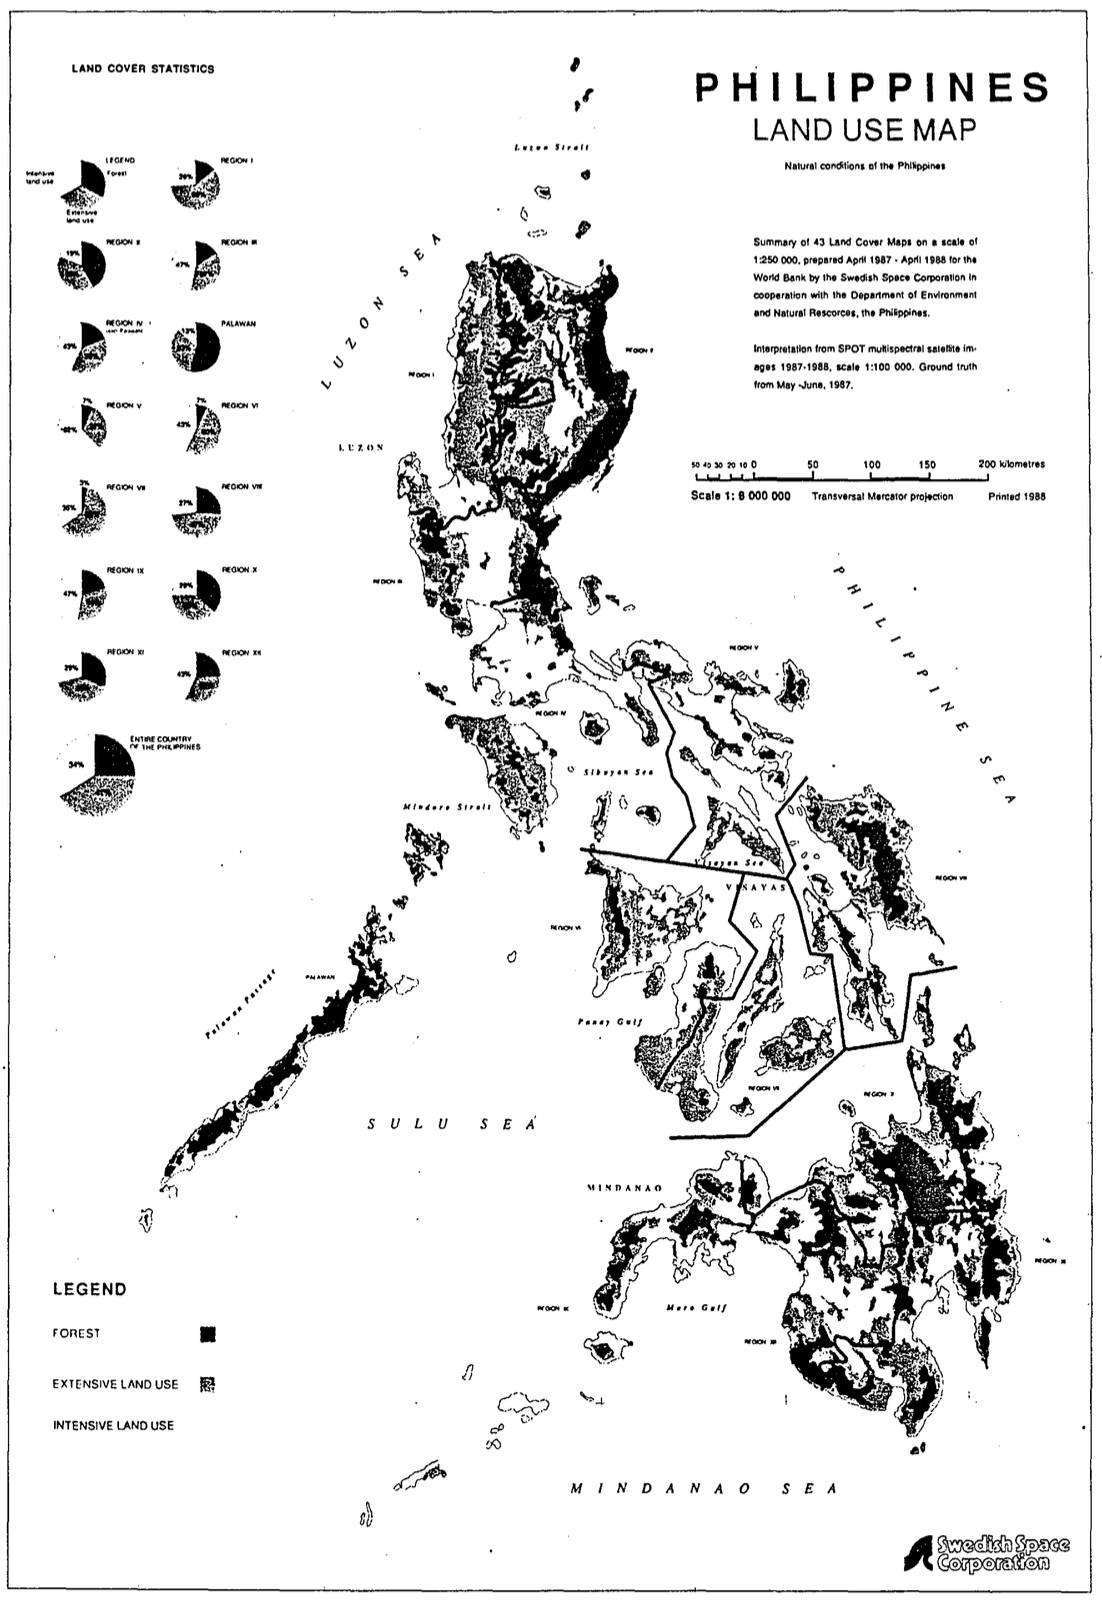
\includegraphics[width=\textwidth]{fig_1987-lc-map.png}
		\caption[SSC/NAMRIA land cover maps.]{}
		\label{fig: intro-fig1.1a}
	\end{subfigure}
	\begin{subfigure}[t]{0.32\textwidth}
		\includegraphics[width=\textwidth]{fig_2003-lc-map.png}
		\caption[SSC/NAMRIA land cover maps.]{}
		\label{fig: intro-fig1.1b}
	\end{subfigure}
	\begin{subfigure}[t]{0.32\textwidth}
		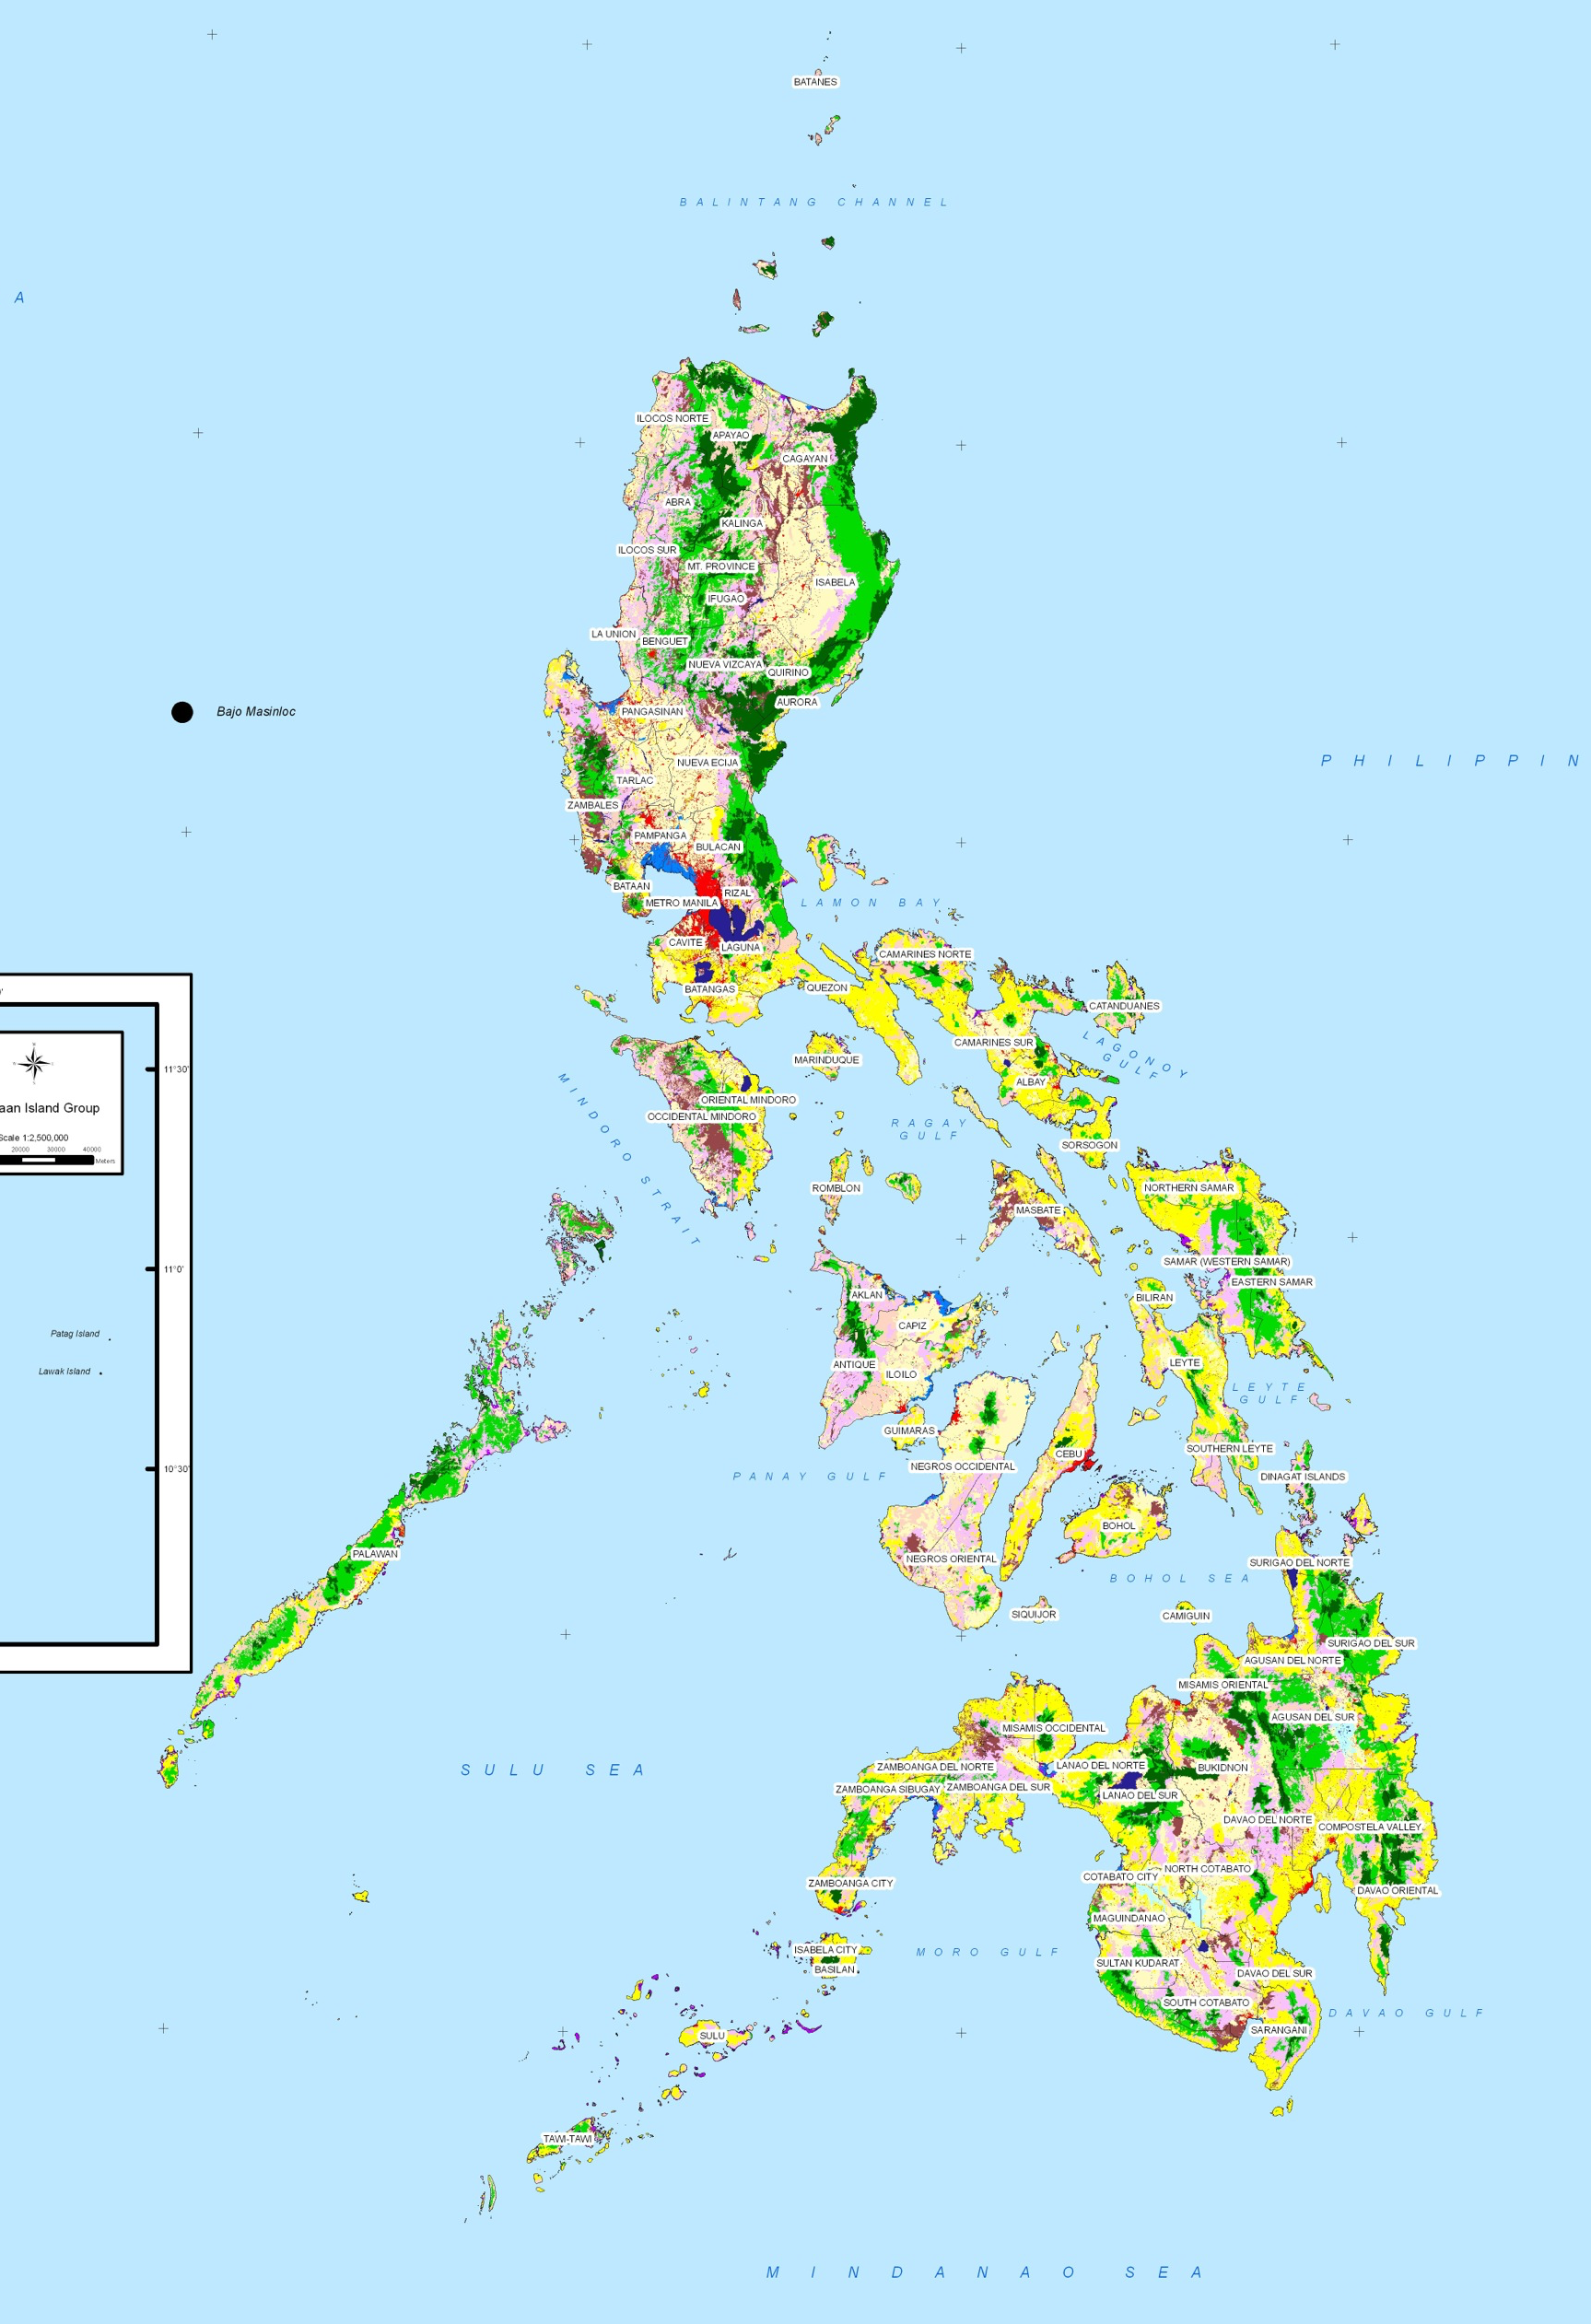
\includegraphics[width=\textwidth]{fig_2010-lc-map.png}
		\caption[SSC/NAMRIA land cover maps.]{}
		\label{fig: intro-fig1.1c}
	\end{subfigure}
	\caption[Recent national land cover maps of the Philippines: (a) 1987 SSC; (b) 2003 NAMRIA; (c) 2010 NAMRIA.]{Recent national land cover maps of the Philippines: (a) 1987 SSC; (b) 2003 NAMRIA; (c) 2010 NAMRIA.}
	\label{fig: intro-fig1.1}
\end{figure}

Finally, there is little known documentation that exists to report on the methods implemented and levels of accuracy achieved in producing many of the forest cover maps from these surveys, except the 1973 and 1987 maps. Lachowski et al. (1979), for the 1973 Landsat-based maps, described the methods undertaken by the mapping work and mentioned an overall accuracy of 85\% to 95\% for the classification of forest types, albeit without sufficient detail. For the 1987 SPOT-based maps, SSC (1988) described their methods and land cover classification system, but did not quantify the accuracy of the results of their interpretation. Kummer (1992b) had cautioned on the reliability of the 1987 SSC map due to major differences with the results of the 1988 Philippine-German Forest Inventory. Reports for other mapping surveys were either not (or no longer) available or were not easily accessible. Since many of these forest mapping surveys employed visual interpretation techniques implemented by expert analysts, the absence of documentation also affects the replicability of the approaches for future work since the knowledge developed from these surveys were ultimately lost.

\section{Overview of the study}
\label{sec: intro-overview-study}

There is an opportunity to explore alternative datasets and methods in support of finding solutions to improve the mapping and monitoring of Philippine forests using remote sensing technology. Synthetic aperture radar (SAR) is an active remote sensing technology that utilises the microwave region of the electromagnetic spectrum that may be used as an alternative (or complement) to optical data for forest mapping and monitoring (discussed in more detail in the next chapter). Innovations in computing technology have leapfrogged over the last two decades and made it possible for computers to handle large remote sensing datasets and to implement sophisticated image processing algorithms for various applications.\\

This research intends to examine the potential of SAR data and digital image processing techniques for mapping forest cover extent and discriminating forest types in the Philippines based on the adopted FAO forest classification system. In contrast to previous national forest mapping surveys using remotely sensed data, which have utilised mainly optical data and visual interpretation for forest cover classification, this study employs image data from an active sensor that can at the onset overcome the limitations brought by persistent cloud cover, and aim to develop a replicable digital image processing and interpretation approach. This study documents the evaluation of the suitability of SAR data for mapping and discriminating forest types by providing quantitative accuracy assessments, and information of the relationships between image data predictor variables and forest types, which are important in developing robust and transparent forest monitoring systems.

This study also adopts the forest categories based on the FAO GFRA for consistency with the recent official national forest cover maps (i.e., 2003 and 2010). One of the key research thrusts in support of planning and decision-making of the National Mapping and Resource Authority (NAMRIA) is to utilise SAR imagery, either as an alternative to or in complementation with optical data, coupled with digital image processing approaches with the aim of developing improved wall-to-wall coverage baseline land and forest cover map products of the entire country on a periodic basis. This study can potentially support NAMRIA’s aims by providing insights on the suitability of radar data and a suite of digital image processing techniques for mapping and monitoring forest extent and forest types in the Philippines.

\section{Thesis structure}
\label{sec: intro-thesis-structure}

This thesis is divided into six chapters. Chapter 1 gives a background of forest ecosystems and remote sensing of forests, and presents an overview of the study. Chapter 2 provides a review of relevant literature on forest applications of synthetic aperture radar, forest classification systems, and the approaches used in this study including cluster analysis, decision trees, texture measures, and object-based image analysis. Chapter 3 describes the study area, the datasets used, and the methods employed. Chapter 4 presents the results of the feature extraction, and clustering and classification procedures. Chapter 5 provides a thorough discussion of the results. Chapter 6 summarizes the study and outlines recommendations for future research and application. The final sections contain the references cited in the text, and the appendices consisting of supplemental figures, rulesets, and scripts used in the study.

	%--------------------------------------------------------------------------
% Literature Review
%--------------------------------------------------------------------------

\chapter{Literature Review}
\label{cha: literature-review}

\section{Synthetic aperture radar for forest applications}
\label{sec: litrev-sar-forest-apps}

Synthetic aperture radar (SAR) is a viable alternative to optical remote sensing for land cover characterisation, mapping, and monitoring to support environmental studies and resource management. SAR systems transmit short pulses of microwave energy toward the Earth’s surface, which then interact with different surface features like vegetation, infrastructure, and water bodies, and the sensor provides information such as backscattering coefficients, which represent the strength of the microwave energy emitted from the antenna and returned after scattering by the target features (\cite{thapa_evaluation_2014}). Backscatter is characterised by polarised modes of the transmitted and received signals, particularly the co-polarisation channels: horizontal transmit and horizontal receive (HH) and vertical transmit and vertical receive (VV); and the cross-polarisation channels: horizontal transmit and vertical receive (HV) and vertical transmit and horizontal receive (VH). Scattering mechanisms that contribute to backscattered energy include surface scattering from water bodies and slightly rough surfaces, double bounce scattering from dihedral surfaces and edges, and volume scattering from forests and other vegetation (\cite{van_zyl_unsupervised_1989}; \cite{freeman_three-component_1998}).

SAR sensors are unaffected by atmospheric conditions and can penetrate through clouds, haze, and smoke, thereby overcoming limitations of optical data in cloudy tropical regions (\cite{achard_estimating_2010}; \cite{shimada_generating_2010}). As an active remote sensing system, radar imagery can be calibrated to a very high degree of accuracy with its constant illumination geometry and well-established transmit/receive power spectra; hence allowing the comparison of backscatter values ($\sigma$\textsuperscript{0}) over time and space (i.e., structurally and electrically similar vegetation have the same backscattering behaviour anywhere on earth; \cite{kellndorfer_toward_1998}). SAR data can be acquired consistently on a repetitive basis regardless of weather conditions; hence, these data can potentially be used to complement or replace optical remote sensing systems in an operational programme for mapping and monitoring of forests (\cite{almeida-filho_detecting_2007}).

Notable studies, as described next, were aimed at understanding the relationships between SAR data and forest structure to explore the utility of SAR for forest applications. Ulaby et al. (\citeyearpar{ulaby_textural_1986}) studied the suitability of radar data from two L-band SAR missions, Seasat and the Shuttle Imaging Radar (SIR-A), for mapping forest types in North and South America. They found that combining backscatter and texture measures improved discrimination of forest types using supervised classification techniques. Durden et al. (\citeyearpar{durden_modeling_1989}) described a theoretical scattering mechanism model for forested areas and found good agreement between modelled polarisation signatures with observed polarisation measurements using ground data and AIRSAR L-band data. Le Toan (\citeyearpar{le_toan_relating_1992}) analysed the relationships of multi-frequency (i.e., C, L, and P bands) quad-polarimetric (i.e., HH, HV, VH, VV) AIRSAR data with forest stand parameters measured from pine forests ranging from young to mature stages, which revealed that longer wavelength SAR data, particularly P- and L-bands, had strong correlations and high sensitivities to forest biomass. Moreover, cross-polarised signals showed high correlations with forest stand parameters. Imhoff (\citeyearpar{imhoff_theoretical_1995}) investigated the effect of forest structural differences in equal-biomass broadleaf forest stands on radar backscatter similarly from multi-frequency quad-polarimetric AIRSAR data. The results indicated that structure exerted a substantial effect on backscatter, which tended to increase with forest structural consolidation into fewer and larger parts; hence providing a structural link to positive correlations of radar backscatter with aboveground biomass. Woodhouse et al. (\citeyearpar{woodhouse_radar_2012}) believes that \enquote{radar is typically the best satellite-based remote sensing tool for mapping forest extent, estimating forest structural variability, and detecting deforestation and degradation.}

The Advanced Land Observing Satellite (ALOS), launched on 24 January 2006, was developed for detailed observation of the Earth’s surface and frequent monitoring of global environmental changes, such as forest ecosystems, using both optical and SAR sensors (\cite{shimada_advanced_2010}). Onboard ALOS is the Phased Array type L-band Synthetic Aperture Radar (PALSAR), a multi-polarisation L-band SAR system, which builds on the experience gained from its predecessor, the Japan Earth Resources Satellite (JERS-1), similarly a spaceborne L-band SAR sensor that was successfully used for global rainforest and boreal forest mapping projects in the 1990s (\cite{rosenqvist_global_2000}; \cite{rosenqvist_overview_2004}). L-band SAR (\url{~}25 cm wavelength) is particularly useful in mapping forest areas due to its longer wavelengths and shorter frequencies (\cite{thapa_evaluation_2014}), which in turn allows greater penetration through forest vegetation by the transmitted signal and sensitivity for detecting deforestation (i.e., L-band backscatter is typically lower in non-forest areas compared to forests) and forest inundation (i.e., L-band backscatter is typically lower in inundated forest areas); thereby yielding important information for forest cover monitoring (\cite{shimada_advanced_2010}; \cite{shimada_generating_2010}). The co-polarised channel (i.e., HH) has been found to be sensitive to vertical structure, such as regrowth in clear-cut regions, while the cross-polarised channel (i.e., HV) is less sensitive to vertical structure in low vegetation or clear-cut areas (\cite{shimada_advanced_2010}). ALOS also featured a unique systematic observation strategy to provide consistent, semi-annual, wall-to-wall observations at fine spatial resolution of the Earth's entire landmass during the satellite's lifetime (\cite{rosenqvist_alos_2007}).

Since its launch, ALOS/PALSAR data have been used for various forest applications such as detecting tropical deforestation (\cite{almeidafilho_using_2009}; \cite{rahman_mapping_2010}; \cite{whittle_detection_2012}; \cite{motohka_using_2014}); time-series mapping of forest cover (\cite{thapa_tropical_2013}; \cite{shimada_new_2014}); assessing forest fragmentation (\cite{dong_50-m_2014}); estimating mangrove biomass (\cite{hamdan_l-band_2014}) and forest aboveground biomass (\cite{mitchard_using_2009}; \cite{morel_estimating_2011}; \cite{sarker_potential_2012}; \cite{cartus_mapping_2012}; \cite{rahman_retrieval_2013}; \cite{mermoz_decrease_2015}; \cite{thapa_potential_2015}); mapping mangrove areas (\cite{rocha_de_souza_pereira_mapping_2012}) and changes in mangrove extent (\cite{nascimento_mapping_2013}); and assessing processes of forest disturbances and successional dynamics (\cite{joshi_mapping_2015}; \cite{mermoz_forest_2016}). PALSAR is also one of the main data sources for the Task on Forest Carbon Tracking, established by the Group on Earth Observation in 2009 as a global forest monitoring system in support to the United Nations Framework Convention on Climate Change post-Kyoto Protocol framework (\cite{shimada_advanced_2010}).

\section{Land and forest cover type mapping using\\ ALOS/PALSAR}
\label{sec: litrev-forest-mapping-palsar}

Studies have demonstrated the use of ALOS/PALSAR for mapping tropical forest types and broad land cover categories, which is the topic of interest of this study. For example, quad-polarimetric PALSAR data were used for mapping broad land cover categories. Rahman and Sumantyo \citeyearpar{rahman_mapping_2010} mapped forest, forest re-growth, upland soil/shrub, lowland soil, settlement, and water/wetlands in Southern Chittagong, Bangladesh. They found that forests were discriminated well from other land cover categories, although forest re-growth was not detected, and only a 66\% overall classification accuracy was achieved. Mishra et al. \citeyearpar{mishra_land_2011} tested different classifiers for mapping broad land cover types (i.e., tall vegetation, short vegetation, urban, bare soil, and water) in Roorkee, India. Their results showed that decision tree classifier obtained an 86\% overall accuracy and performed better than other classification techniques. Avtar et al. \citeyearpar{avtar_characterization_2012} assessed two images for characterising forest types (evergreen, deciduous, sparsely deciduous) and deforestation in Northern Cambodia. Their study showed that HV-polarised backscatter coefficient, cross-polarisation ratio (HH/HV), among other parameters gave better results for characterising forest types. Further, they observed that HV-polarised backscatter coefficient of evergreen forest was higher compared to deciduous and sparsely deciduous forest types, particularly due to the multiple canopies of evergreen forests that enhance volume scattering.

Previous studies have used dual-polarised PALSAR data combined with texture information derived from the radar images. Longépé et al. \citeyearpar{longepe_assessment_2011} mapped land cover types (i.e., dry forest, wet forest, acacia, clear cut, oil palm, others) in Riau province, Sumatra, Indonesia using dual-polarised (HH, HV) PALSAR data and texture measures. The overall agreement with reference data was \url{~}70\% for land cover classification and \url{~}87\% for natural forest discrimination. Similarly, Rakwatin et al. \citeyearpar{rakwatin_using_2012} mapped broad land cover types (i.e., forest, oil palm, acacia, clear cut, water) in Riau province, Indonesia, and reported a 73\% overall classification accuracy. The overall accuracies for land cover classification increased by about 10\% when combined with texture information. Li et al. \citeyearpar{li_comparative_2012} used dual-polarised PALSAR data and texture measures for mapping broad land cover types (i.e., forest, succession, agropasture, water, wetland, urban) in Altamira, Para, Brazil. The best classification resulted in a 74\% overall accuracy, of which textural information was valuable for improving vegetation classification. They also reported difficulties in discriminating between forest classes and between forest succession classes.

Discriminating tropical forest types based on successional stages have been studied due to its importance in understanding the role of forest regeneration in global carbon cycles. Li et al. \citeyearpar{li_comparative_2012} found that neither L-band PALSAR nor C-band RADARSAT-2 dual-polarisation data can accurately separate between detailed forest types (upland, flooding, liana) and between forest succession stages (initial, intermediate, advanced). Upon testing different classifiers, they also found that no algorithm could successfully separate forest succession stages. Liesenberg \& Gloaguen \citeyearpar{liesenberg_evaluating_2013} evaluated different PALSAR data modes (e.g., single-, dual-, quad-polarimetric, and interferometric) to characterize and classify primary, successional secondary, and riparian forest classes in Eastern Amazon, Brazil. They found that while quad-polarised data provided better results compared to single or dual-polarised data, the overall accuracies remained low. Radar backscatter of primary and riparian forests were higher than those observed for successional secondary forest types (initial, intermediate, advanced). Backscatter values tended to increase from advanced to initial secondary stage forest, although no substantial differences were observed between successional secondary forest types.

\section{Forest classification systems}
\label{sec: litrev-forest-class-system}

\subsection{FAO Global Forest Resources Assessment forest classification}

The above examples on mapping forest cover types using ALOS/PALSAR data have adopted classification schemes based on forest age or successional stages (e.g., primary, secondary), disturbance gradients (e.g., pristine, degraded), or on bespoke classes suited to the area of interest. However, using different classification schemes makes compatibility between datasets difficult to ascertain and hinders the comparative analysis of land cover types across space and time in a consistent manner (\cite{ahlqvist_search_2008}). Although, at present, no definitive universally accepted land cover classification system exists (Townshend et al., 2010), such a classification system is crucial for the evaluation, comparison, and change analysis of land cover products (\cite{giri_brief_2012}).

The Global Forest Resources Assessments (GFRA), coordinated by FAO at the request of its member countries, provides periodic information on the situation of the world's forests to support decision-making in investment and policymaking in forestry and sustainable development (\cite{fao_global_2015}). One of the primary sources of data for these assessments is the Country Report prepared by national correspondents, which are based on National Forest Assessments (NFA) and are submitted to FAO for consolidation in a global report produced every 5 years. Forest inventories, which are based on systematic field sampling and complemented by remote sensing, are the primary means for data collection within these NFAs. The FAO formulates guidelines for country reporting, including forest classification terms and definitions, to ensure compatibility and interoperability of information across countries and time for global forest resources monitoring, as well as facilitating comparative analysis of land cover change within national-level assessments.

In the Philippines, national remote sensing surveys were conducted by NAMRIA to complement national forest inventories for the reporting periods in 2005 and 2010 (i.e., 2003 and 2010 land cover map products), which adopted the FAO GFRA classification and definitions (Table \ref{tab: intro-table2.1}). Forest inventories were only implemented for the 2005 reporting, but were not carried out for the 2010 reporting (\cite{fao_2010_2010}). For consistency, this study similarly adopted the same forest classification system for evaluating L-band PALSAR data for distinguishing forest cover types based on this system, which would allow comparison with the official land cover maps.\\

\begin{spacing}{1.0}
\begin{longtable}[h!]{ p{3.5cm} p{10.5cm} }

    \caption[Global Forest Resources Assessment categories and definitions.]{Categories and definitions based on the Global Forest Resources Assessment (Source: \cite{fao_2005_2005}; \cite{fao_2010_2010}).}
    \label{tab: intro-table2.1}\\
    
    \toprule
    Category & Definition \\
    \midrule
    \endhead

    Forest & Land with tree crown cover (or equivalent stocking level) of more than 10\% and area of more than 0.5 ha. \\[5pt]
    Broadleaved forest & Forest with predominance (more than 75\% of tree crown cover) of trees of broadleaved species.\\[5pt]
    Coniferous forest & Forest with predominance (more than 75\% of tree crown cover) of trees of coniferous species.\\[5pt]
	Bamboo/palm formations & Forest on which more than 75\% of the crown cover consists of tree species other than coniferous or broadleaved species (e.g. tree-form species of the bamboo, palm and fern families).\\[5pt]
	Mixed forest & Forest in which neither coniferous, nor broadleaved, nor palms, bamboos, account for more than 75\% of the tree crown cover.\\[5pt]
	Closed forest ($\geq$ 40\%) & Natural forest where trees in the various storeys and undergrowth cover 40\% of the ground. These formations do not have a continuous dense grass layer. They are either managed or unmanaged forests primary or in an advanced state of reconstitution and may have been logged-over one or more times, having kept their characteristics of forest stands, possibly with modified structure and composition. Typical examples of tropical closed forest formations include tropical rainforest and mangrove forest.\\[5pt]
	Open forest (10 to \textless 40\%) & Formations where trees form a discontinuous layer covering 10 to 40\% of the ground. This forest usually includes a continuous grass layer allowing grazing activities and the spreading of fires.\\[5pt]
	Forest plantation & Forest stands established by planting or/and seeding in the process of afforestation or reforestation. They are either of introduced species (all planted stands), or intensively managed stands of indigenous species, which meet all the following criteria: one or two species at plantation, even age class, regular spacing.\\[5pt]
	Open broadleaved forest plantation (10 to \textless 40\%) & Forest plantation where the crown cover is between 10 and 40\% of the area.\\[18pt]
	Closed broadleaved forest plantation ($\geq$ 40\%) & Forest plantation where the crown cover is above or 40\% of the area.\\[18pt]
	Other wooded land & Land either with a crown cover (or equivalent stocking level) of 5 to 10\% of trees able to reach a height of 5 m at maturity in situ; or a crown cover (or equivalent stocking level) of more than 10\% of trees not able to reach a height of 5 m at maturity in situ (e.g., dwarf or stunted trees); or with shrub or bush cover of more than 10\%.\\[5pt]
	Shrubs & Refers to vegetation types where the dominant woody elements are shrubs i.e. woody perennial plants, generally of more than 0.5 m and less than 5 m in height on maturity and without a definite crown. The height limits for trees and shrubs should be interpreted with flexibility, particularly the minimum tree and maximum shrub height, which may vary between 5 and 7 m approximately.\\[5pt]
	Fallow & It encompasses forest fallow where the woody vegetation is under 5 m in height. It refers to woody vegetation deriving from the clearing of natural forest for shifting agriculture. It is part of a forest fallow consisting of a mosaic of various reconstitution phases. The vegetation does not reach a height of 5 m.\\[5pt]
	Wooded grasslands (5 to \textless 10\%) & Land where the trees cover between 5 to 10\% of the area and their height may reach 5 m at maturity.\\[3pt]
	Other land & Land not classified as forest or other wooded land, as described above. Including cultivated land, grasslands and pastures, built-up areas, barren land etc.\\[5pt]
	Inland water & Area occupied by major rivers, lakes, and reservoirs.\\[3pt]
	
    \bottomrule
\end{longtable}
\end{spacing}

\subsection{Multi-level hierarchical classification schemes}

According to Di Gregorio \citeyearpar{di_gregorio_land_2005}, a hierarchically structured land cover classification offers more consistency due to its ability to accommodate different levels of information (i.e., beginning with broad-level classes that are systematically subdivided into detailed sub-classes). The following examples describe some of the early development and full implementations of multi-level hierarchical land cover classification schemes applied to SAR data.

Pierce et al. \citeyearpar{pierce_knowledge-based_1994} and Dobson et al. \citeyearpar{dobson_knowledge-based_1996} were among the initial studies that implemented a \enquote{knowledge-based} approach for classifying land cover types using polarimetric AIRSAR data over Northern Michigan. The design of the approach uses knowledge of the nature of radar backscatter from target features to formulate decision rules for classification in a sequential format. The land cover classes were defined on the basis of simple structural attributes of widespread applicability, relying heavily on their expert knowledge, and decision rules were determined empirically using training data to define simple thresholds (\cite{dobson_knowledge-based_1996}). Their knowledge-based classifier operated sequentially at each level of the class hierarchy. Overall accuracies above 90\% were reported from the results of the classification by both studies.

In another study, Walker et al. \citeyearpar{walker_large-area_2010} devised a bespoke hierarchical, five-level land cover classification scheme (see Fig. \ref{fig: litrev-fig2.1}) for large-area land and forest cover classification and mapping of the Xingu watershed in the Brazilian Amazon using dual-polarised PALSAR data and feature extraction (such as texture measures). Starting from detailed land cover types at the first level, classes were aggregated in each subsequent level until the last level, which consisted of forest and non-forest classes. The forest sub- categories were forest and \textit{cerrado}, each of which were further sub-categorised into intact, degraded, or regenerating forests. Overall accuracies were low at the detailed classification level (58\% at 15 classes), which increased as classes were aggregated at subsequent levels, eventually obtaining a high accuracy at the broad classification level (92\% at 2 classes).

\begin{figure}
	\centering
	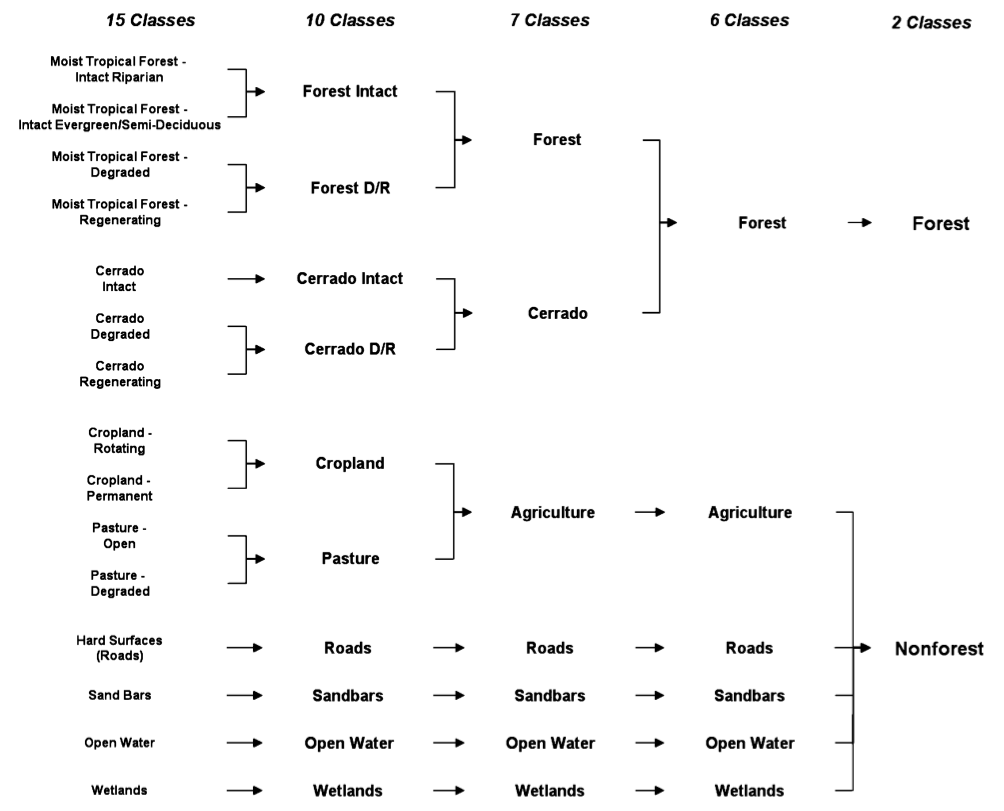
\includegraphics[width=1.0\textwidth]{fig_walker-hierarchy.png}
	\caption[Multi-level hierarchical classification system.]{Multi-level hierarchical classification system adopted by Walker et al. \citeyearpar{walker_large-area_2010}.}
	\label{fig: litrev-fig2.1}
\end{figure}

Currently, one of the most comprehensive, flexible, and internationally applied framework for land cover characterisation is the United Nations (UN) Land Cover Classification System (LCCS) developed by FAO (\cite{giri_brief_2012}). The UN LCCS was developed in response to a need for reliable, harmonised, and standardised information on land cover and land cover change (\cite{di_gregorio_land_2005}). It provides descriptors of land cover classes through a dichotomous, modular, hierarchical system for translation between typologies (\cite{defourny_revisiting_2012}) such that the comparison of land cover products, including qualitative and quantitative evaluations of product differences, are enabled (\cite{kuenzer_comparing_2014}). The first fully operational version of the UN LCCS was developed initially for the implementation of the AFRICOVER project (\cite{kalensky_africover_1998}; \cite{herold_evaluating_2012}). Some global land cover products that are compliant with the UN LCCS standards include the GLC2000 (\cite{bartholome_glc2000:_2005}) and GlobCover (\cite{arino_globcover:_2007}).

Two studies described as follows used PALSAR data for FAO LCCS-compliant land and forest cover mapping. Hoekman et al. \citeyearpar{hoekman_palsar_2010} mapped forest and land cover types in sub-continental Borneo using single- and dual-polarised PALSAR data in 2007. The resulting demonstration product was 85.5\% in full agreement with an independent reference dataset. The map legend consisted of 22 classes, including eight forest types, namely: tropical lowland forest, broadleaved evergreen; tropical mountain forest, broadleaved evergreen; riverine forest; swamp forest; mangrove forest; nipah mangrove forest; peat swamp (pole) forest; peat swamp (\textit{padang}) forest; and forest mosaics/fragmented or degraded forest. Except for nipah mangrove forest, the degree of full agreement was very high for lowland forest and fair/good for other natural forest types.

Another study by Otukei et al. \citeyearpar{otukei_using_2014} mapped land cover types in Bwindi Impenetrable National Park, Uganda based on the FAO Africover LCCS using quad- polarimetric ALOS/PALSAR data. The legend consisted of eight land cover types including dense evergreen forest, dry bare farmland, wet bare farmland, mixed farmland, mixed rangeland, degraded wetland, aquatic vegetation, and open water. An overall classification accuracy of 86\% was achieved, of which mixed rangeland and farmland were found to be the least discriminated.

While these studies and implementations, including the FAO GFRA-based land cover/forest type classification (see Appendix \ref{tab: appendix-table.a1}), applied hierarchically structured classification approaches, the determination of the sequence and order of the classes in these hierarchies were heuristically determined based on expert knowledge or on what made logical sense (i.e., similar to the \enquote{classification logic} proposed by Running et al. \citeyearpar{running_remote_1995} and implemented by DeFries et al. \citeyearpar{defries_global_1998} and Hansen et al. \citeyearpar{hansen_global_2000} for generating AVHRR-based global land cover products). For this study, a hierarchical clustering analysis was implemented (described in more detail in the next section) to determine a natural hierarchy of forest cover classes based on the multi-year PALSAR data, which would then define the multi-level class hierarchy to guide the execution of the classification.

\section{Cluster analysis}
\label{sec: litrev-cluster-analysis}

Cluster analysis, or clustering, is the art of finding groups or structure in the data (\cite{kaufman_introduction_1990}). The purpose of cluster analysis is to group observations into clusters in such a way that observations in the same cluster are more similar to one another than they are to observations in other clusters (\cite{bajorski_statistics_2011}). Cluster analysis, also often called unsupervised learning, does not require prior information about the groupings of observations and is commonly employed for descriptive or exploratory purposes to better understand the structure of the data (\cite{bajorski_statistics_2011}).

To measure the degree of similarity or dissimilarity between observations, distances are computed on the basis of their proximity in two-dimensional space in such that the smaller the distance between observations represents greater similarity and larger distances as less similarity (\cite{hair_multivariate_2013}). Euclidean distance is the most commonly used measure of similarity between two observations (\cite{kaufman_introduction_1990}), which is essentially a measure of the length of a straight line drawn between two observations when shown graphically.

\begin{figure}
	\centering
	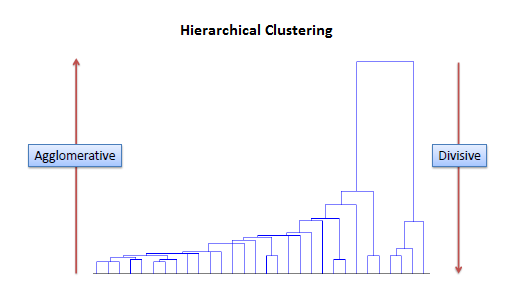
\includegraphics[width=1.0\textwidth]{fig_hierarchical-clustering.png}
	\caption[A dendrogram with arrows showing agglomerative and divisive hierarchical clustering techniques.]{A dendrogram with arrows showing agglomerative and divisive hierarchical clustering techniques (Source: Sayed, \citeyear{sayed_hierarchical_2016}).}
	\label{fig: litrev-fig2.2}
\end{figure}

There are two types of clustering procedures: hierarchical and non-hierarchical (or partitioning). Non-hierarchical clustering procedures divide the observations into a pre- defined number of clusters, which can be defined by the user or calculated within the algorithm (\cite{bajorski_statistics_2011}). The K-means is one of the most commonly used algorithms for non-hierarchical methods, which works by partitioning observations into a specified number of clusters and iteratively reassigns observations until a criteria for cluster homogeneity is met (\cite{hair_multivariate_2013}).

Hierarchical clustering procedures, on the other hand, do not require observations into a pre-defined number of clusters. The result is a tree structure, more commonly known as a dendrogram (see Fig. \ref{fig: litrev-fig2.2}), which is a graphical representation of the results of the hierarchical procedure that shows how the clusters are combined at each step of the procedure until all are contained in a single cluster (Hair et al., 2013). The dendrogram is a one-dimensional display of similarity with the height of the join indicating dissimilarity (\cite{ripley_pattern_1996}). According to Bajorski \citeyearpar{bajorski_statistics_2011}, hierarchical clustering methods often provide more clustering information than other methods.

Johnson \citeyearpar{johnson_hierarchical_1967} provided a succinct outline of the hierarchical clustering process. Given a dataset of N observations to be clustered and NxN distance (or similarity) matrix:

\begin{enumerate}
	\item Assign each observation to its own cluster, i.e., N observations will be equal to N clusters. Let the distances (or similarities) between clusters equal the distances similarities between observations they contain;
	\item Search for the closest (most similar) pair of clusters and combine them into a single cluster, such that there is one less cluster;
	\item Compute the distances (similarities) between the new cluster and each of the old clusters;
	\item Repeat steps \#2 and \#3 until all items are grouped into a single cluster of size N.
\end{enumerate}

In hierarchical clustering procedures, there are two types of methods: agglomerative and divisive (\cite{kaufman_introduction_1990}). These two methods construct their hierarchy in opposite directions (Fig. \ref{fig: litrev-fig2.2}). Divisive methods begin with all observations under one cluster and subsequently divide the data into the two meaningful clusters, then the process continues until the number of clusters is achieved. Agglomerative methods start with each observation forming a separate cluster, and are subsequently merged into the most similar clusters until all observations are in a single cluster.

The algorithm used in a hierarchical clustering procedure defines how similarity is measured in the clustering process (\cite{hair_multivariate_2013}). There are numerous algorithms for agglomerative methods, which only vary in their definition of between-cluster dissimilarity (\cite{kaufman_introduction_1990}). Some of the most common methods include (\ref{fig: litrev-fig2.3}): single linkage, complete linkage, and average linkage, which are described as follows (\cite{podani_introduction_2000}; \cite{bajorski_statistics_2011}; \cite{hair_multivariate_2013}):

\begin{itemize}
	\item Single linkage algorithm (also called minimum distance or nearest neighbor algorithm) defines similarity as the distance between the two closest elements between two clusters;
	\item Complete linkage algorithm (also called maximum distance or farthest neighbor algorithm) defines similarity as the distance between the two farthest elements from the two clusters; and
	\item Average linkage algorithm (also called average distance or unweighted pair-group average method) defines similarity as the average distance over all possible pairs of elements from the two clusters. The average linkage method gives a more robust solution compared to the two other techniques (\cite{sokal_principles_1963}; \cite{johnson_hierarchical_1967}).
\end{itemize}

\begin{figure}[!ht] \centering
	\captionsetup[subfigure]{width=2.0in} % <-- Use this to control text which is poorly spaced under a subfigure. 
	\begin{subfigure}[t]{0.32\textwidth}
		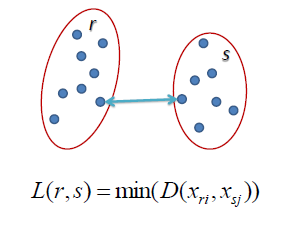
\includegraphics[width=\textwidth]{fig_clustering-single.png}
		\caption[Linkage methods in clustering.]{}
		\label{fig: litrev-fig2.3a}
	\end{subfigure}
	\begin{subfigure}[t]{0.32\textwidth}
		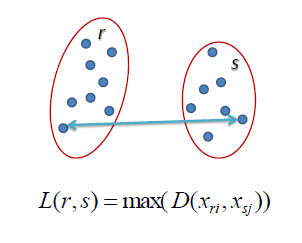
\includegraphics[width=\textwidth]{fig_clustering-complete.png}
		\caption[Linkage methods in clustering.]{}
		\label{fig: litrev-fig2.3b}
	\end{subfigure}
	\begin{subfigure}[t]{0.32\textwidth}
		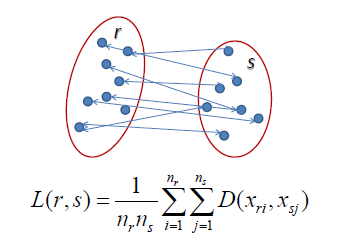
\includegraphics[width=\textwidth]{fig_clustering-average.png}
		\caption[Linkage methods in clustering.]{}
		\label{fig: litrev-fig2.3c}
	\end{subfigure}
	\caption[Methods for computing the distance matrix: (a) single linkage; (b) complete linkage; (c) average linkage.]{Methods for computing the distance matrix: (a) single linkage; (b) complete linkage; (c) average linkage (Source: Sayed, 2016).}
	\label{fig: litrev-fig2.3}
\end{figure}

In Fig. \ref{fig: litrev-fig2.3}, \textit{x} pertains to a set of objects within clusters \textit{r} and \textit{s}, of which \textit{L} is the distance between two clusters that may be defined as the shortest (single) or longest (complete) distance between two points in each cluster, or the average distance between each point in n number of points in one cluster to every point in the other cluster. A distance matrix \textit{D} is calculated where the \textit{i}th row and \textit{j}th column is the distance between the \textit{i}th and \textit{j}th elements.

Hierarchical clustering approaches to data classification are well-established in the biological sciences (i.e., numerical taxonomy) and the humanities (e.g., sociology, psychology), of which the common application is classification according to the relationships among the data observations being clustered (\cite{kaufman_introduction_1990}; \cite{podani_introduction_2000}).

In this study, a hierarchical agglomerative clustering procedure was implemented to determine and visualise the \enquote{natural} hierarchical structure of forest types based on the data with the aim of defining the forest classification hierarchy in contrast to the heuristic approaches such as those implemented by Pierce et al. \citeyearpar{pierce_knowledge-based_1994} and Dobson et al. \citeyearpar{dobson_knowledge-based_1996} to define classification hierarchies. The dendrograms from the cluster analyses were also compared to assess temporal consistency of the multi-year PALSAR mosaics.

\section{Decision tree classification}
\label{sec: litrev-decision-tree}

Classification of SAR data using traditional statistical techniques makes use of the unique local statistics of each image, which in turn necessitates local training and validation of each image; hence limiting its application at regional or global scales (\cite{dobson_knowledge-based_1996}). Knowledge-based or decision tree approaches were found to be more suitable for classifying SAR data (\cite{pierce_knowledge-based_1994}; \cite{dobson_knowledge-based_1996}). This is because decision tree classifiers apply hierarchical decision rules to differentiate land cover classes, and these decision rules or classifiers, once trained, become applicable to other images irrespective of scale and time (\cite{dobson_knowledge-based_1996}).

The decision tree algorithm, or classification and regression trees (CART), is based on the seminal work of Breiman et al. \citeyearpar{breiman_classification_1984}. The decision tree classifier is a simple, non-parametric, binary recursive partitioning procedure in the form of hierarchical rules that are successively applied to the input data or feature space (\cite{strobl_introduction_2009}). The goal of the recursive partitioning is to use a set of predictor variables to estimate the means of one or more response variables; thereby constructing a nested binary tree from the repeated splitting of the data into homogenous subsets (\cite{michaelsen_regression_1994}). The full dataset (parent node) is partitioned into two groups based on a single predictor variable. Each resulting subset (child node) is further partitioned such that the variability in the response variables are minimised and the nodes contain more homogenous observations (\cite{berk_classification_2008}). Once partitioning is complete, the means of the response variables in each terminal node serve as rules for predicting future observations (\cite{michaelsen_regression_1994}; \cite{berk_classification_2008}; \cite{strobl_introduction_2009}).

Decision trees can grow to their maximum size since the splitting of each node continues recursively without a stopping criterion, and eventually the process stops until no further splits are possible due to lack of data (\cite{wu_top_2009}). Larger decision trees have fewer classification errors, hence less bias, but have terminal nodes with few observations, hence greater variance and instability (\cite{berk_classification_2008}). A pruning sequence is then implemented to find a sensible trade-off. Pruning, a process aimed at constraining the size of the tree to avoid overfitting the data, involves removing inefficient branches of the decision tree by consolidating nodes that do not reduce heterogeneity despite the added extra tree complexity (\cite{berk_classification_2008}; \cite{strobl_introduction_2009}). An optimal tree is identified by evaluating the predictive performance of every tree in the pruning sequence either on independent test data or through cross-validation (\cite{wu_top_2009}). Cross-validation, as implemented in this study, involves partitioning the full dataset into subsets, excluding one subset, growing the tree on the remaining data, and testing it on the excluded subset (\cite{michaelsen_regression_1994}). The chances of overfitting is minimised since essentially different data are used to train and test the decision trees.

Several examples have successfully demonstrated the use of decision tree classifiers for the classification of remotely sensed data. With optical data, decision trees have been used for generating global land cover classification map products from the AVHRR sensor (\cite{defries_global_1998}; \cite{hansen_global_2000}); for mapping land and forest cover change in Palawan and Eastern Mindanao in the Philippines from Landsat data (\cite{pereira_forest_2006}); and for mapping decadal mangrove cover change in the Philippines using Landsat (\cite{long_mapping_2013}), among others.

With SAR data, Simard et al. \citeyearpar{simard_use_2000} used decision trees and multi-scale texture measures on the Japan Earth Resources Satellite (JERS-1) SAR data for thematic mapping of tropical forest in Gabon in Central Africa, of which decision trees resulted in improving classification results. Both JERS-1 and the European Resources Satellite (ERS-1) SAR composites were used with a decision tree classifier for mapping land cover in Michigan in the United States (\cite{dobson_knowledge-based_1996}), and for mapping coastal vegetation in Gabon in Central Africa (\cite{simard_mapping_2002}). Dong et al. \citeyearpar{dong_50-m_2014} mapped broad land cover categories (i.e., forest, cropland, urban, water) in Southeast Asia using dual-polarised PALSAR data and a decision tree classifier, and achieved high overall accuracy. The producer's and user's accuracies of forest were 86\% and 93\%, which was partly attributed the simple classification scheme.

Decision trees have a number of advantages over traditional classification methods. Hansen et al. \citeyearpar{hansen_classification_1996} showed that decision trees slightly outperformed maximum likelihood algorithm for classifying monthly composites of AVHRR data. Moreover, decision trees provided an added advantage of reducing data dimensionality by revealing the hierarchical nature of predictor variables, specifically those metrics that contributed to discriminating among cover types. Friedl \& Brodley \citeyearpar{friedl_decision_1997} found that decision tree algorithms consistently outperformed the maximum likelihood and linear discriminant classifiers in terms of classification accuracies applied to global AVHRR data. Pal \& Mather \citeyearpar{pal_assessment_2003} showed that decision trees when applied to Landsat and hyperspectral data performed acceptably well compared to the maximum likelihood and artificial neural network classifiers, except with high-dimensional data. Otukei \& Blaschke \citeyearpar{otukei_land_2010} found that decision trees performed better than maximum likelihood and support vector machines for land cover change assessment using Landsat data. Mishra et al. \citeyearpar{mishra_land_2011} evaluated different classification algorithms for classifying land cover using fully polarimetric ALOS/PALSAR data, and found that decision trees produced more accurate results than parallelepiped, minimum distance, maximum likelihood, and Wishart classifiers.

In this study, a decision tree classifier was used similarly due to its better performance over other classification algorithms, its suitability for classifying SAR data, and its potential applicability of decision rules to images over other areas once the classifier has been trained.

\section{Texture: the grey-level co-occurrence matrices}
\label{sec: litrev-texture-glcm}

Image texture refers to the spatial variability or the patterns of spatial relationships of grey levels (tone) within a neighbourhood of pixels, which is commonly described in terms of roughness or smoothness (Mather \& Koch, 2011). Texture is one of the important elements of image interpretation that are used to describe the characteristics of features in remotely sensed images (Campbell \& Wynne, 2011).

Previous research have utilised different texture information with SAR data for various aspects of land and forest cover type mapping such as improving the discrimination of forest types (Ulaby et al., 1986); detecting clearings in primary forest (Oliver, 2000); discriminating different subcategories of forest vegetation types (Saatchi et al., 2000); mapping of tropical forest (Simard et al., 2000); discriminating inundated vegetation (Podest \& Saatchi, 2002); increasing the accuracy of biomass estimation in tropical forests (Kuplich et al., 2005); and improving the classification accuracies of broad land cover types (Walker et al., 2010; Longépé et al., 2011; Li et al., 2012; Rakwatin et al., 2012).

First- and second-order texture measures are among the descriptors that can be measured in an image. First-order texture measures calculate the spectral variability or statistical moments (e.g., mean, variance, kurtosis, skewness) within a certain window (group of pixels or kernel), of which the moments do not contain any direction (Kurvonen \& Hallikainen, 1999). Second-order texture measures consider the spatial relationships between groups of two neighboring pixels to a certain direction within the window (Gallardo-Cruz et al., 2012). The calculation of second-order texture measures involves the construction of Grey-Level Co-occurrence Matrices (GLCM), which are matrices containing the probabilities of co-occurrence of pixel values for pairs of pixels in a given direction and distance (Gallardo-Cruz et al., 2012).

\begin{figure}
	\centering
	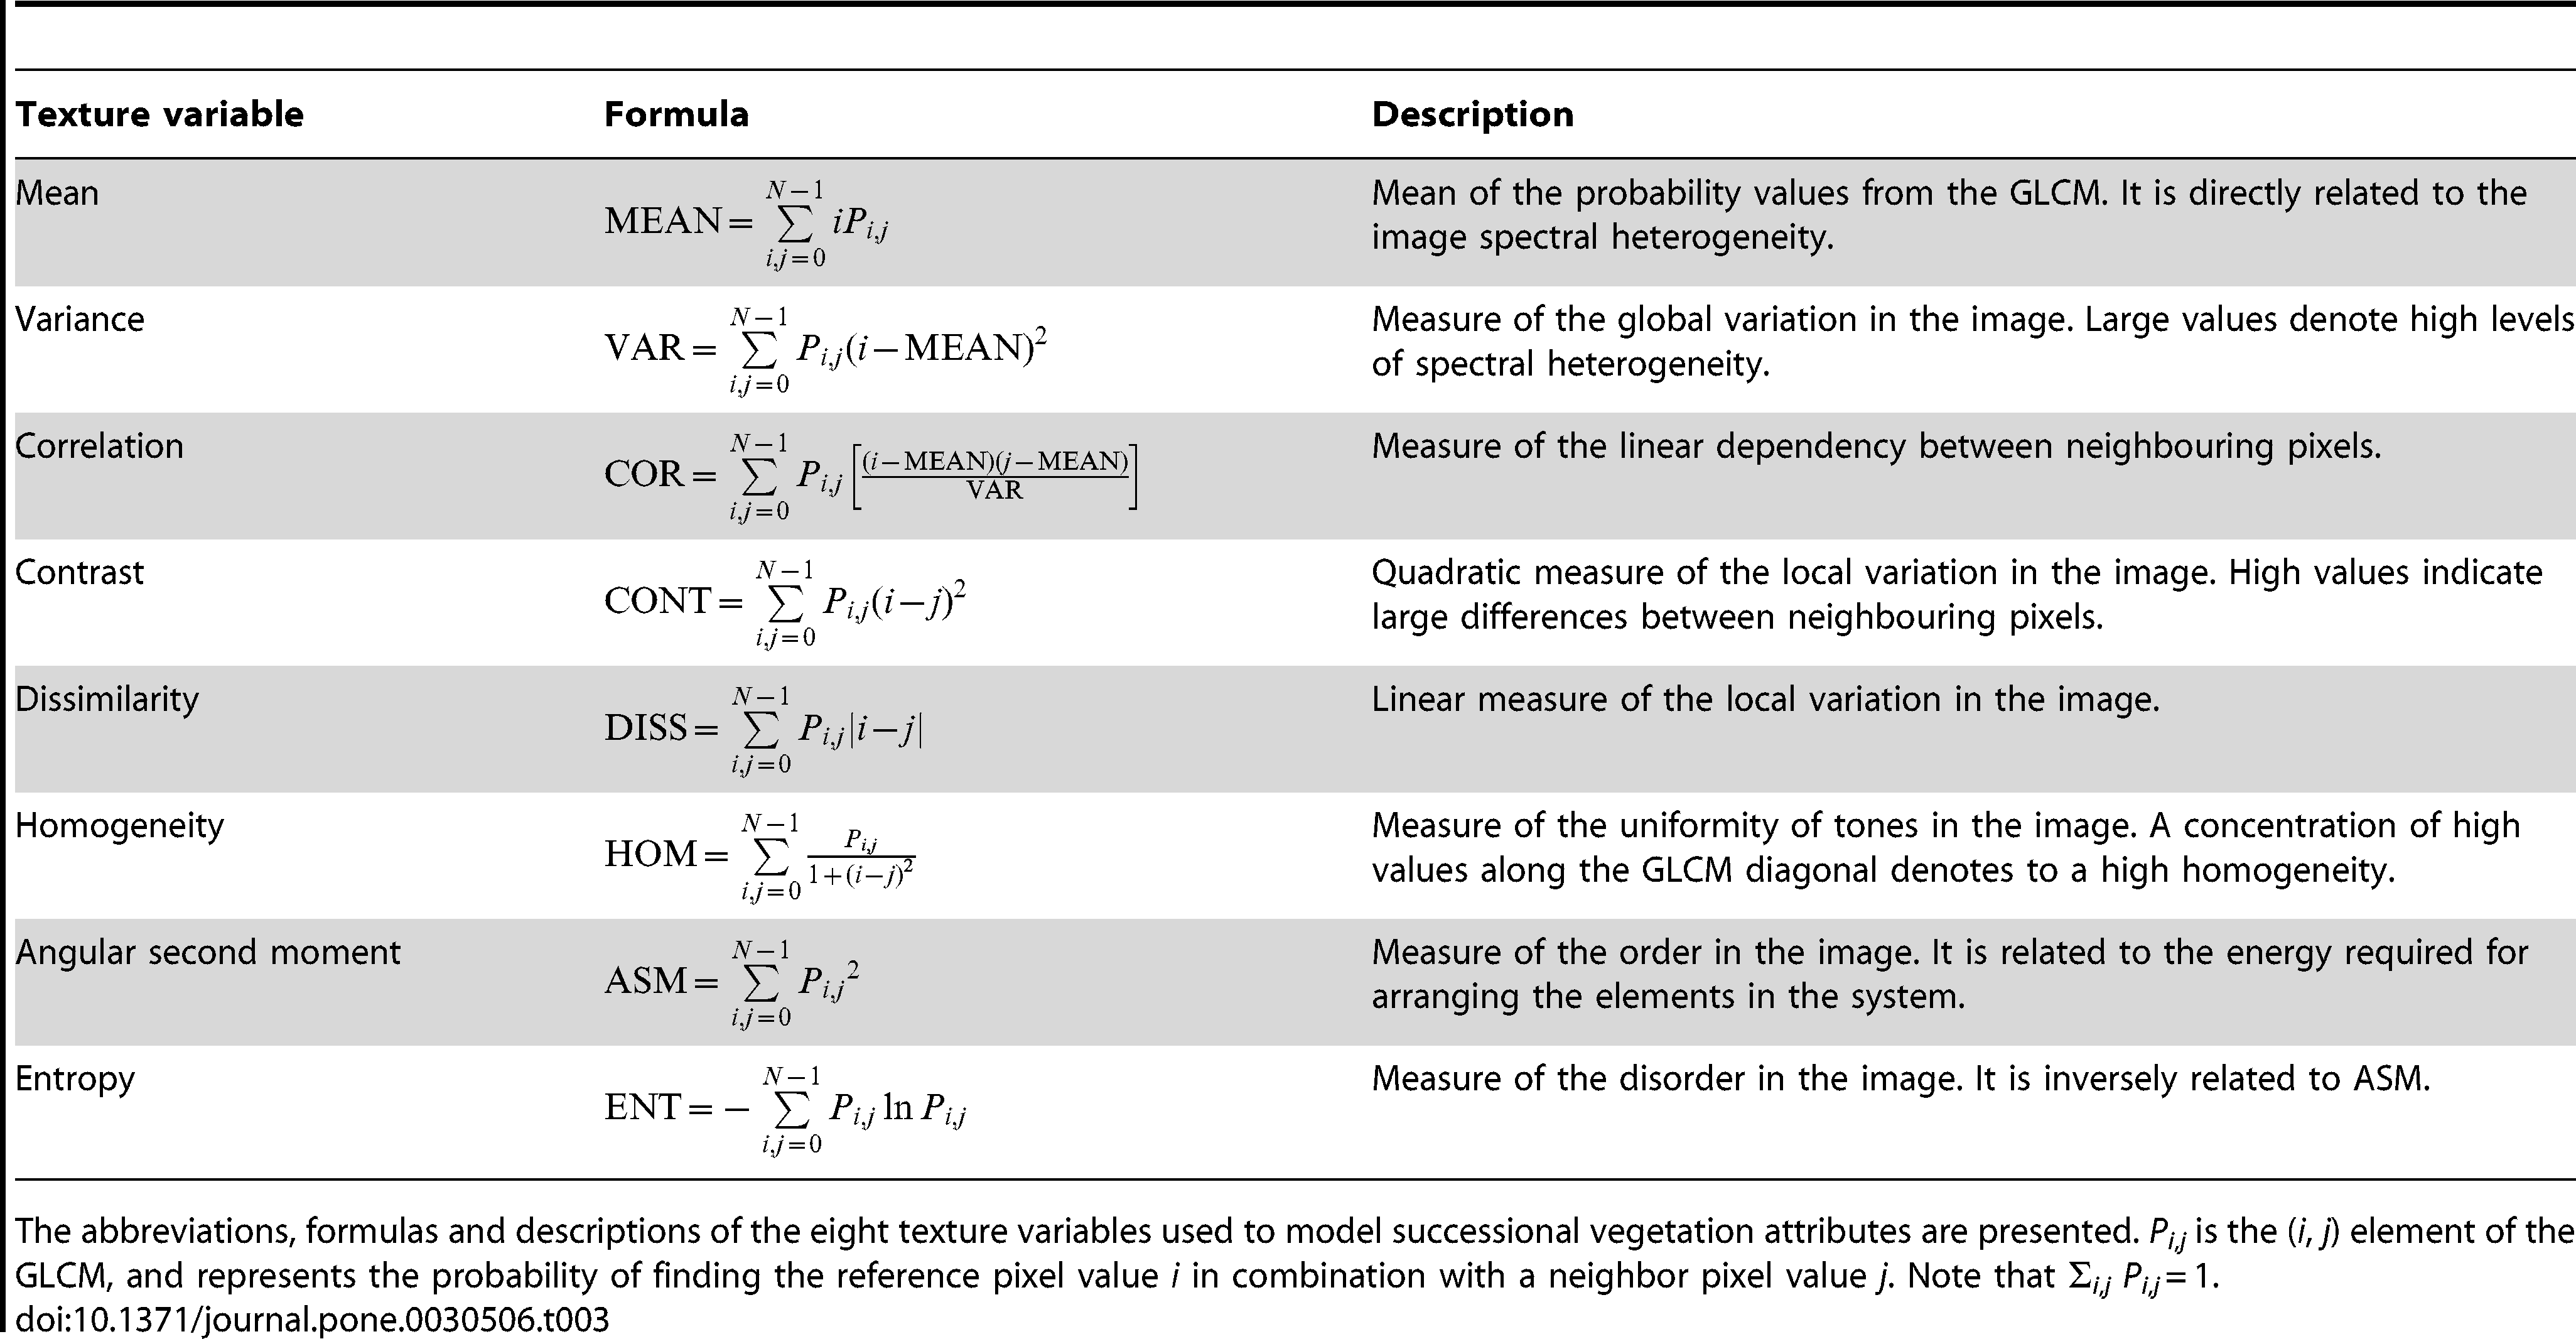
\includegraphics[width=1.0\textwidth]{fig_texture-measures.png}
	\caption[Texture variables derived from the grey-level co-occurrence matrix.]{Texture variables derived from the grey-level co-occurrence matrix (Source: Gallardo-Cruz et al., 2012).}
	\label{fig: litrev-fig2.4}
\end{figure}

The GLCM, a concept first described by Haralick et al. (1973), outlines the distance and angular relationships among a neighbourhood of pixels. It computes the joint probability of occurrence \textit{p(i,j)} of the pairs of grey levels i and j separated by a given distance dij and direction, and the image being initially quantised into \textit{N\textsubscript{g}} grey levels (Haralick et al., 1973). In this study, eight texture variables in three groups were used to describe the degree of contrast between pixels (contrast, dissimilarity, homogeneity), the regularity in the pixels within a neighbourhood of pixels (angular second moment, entropy), and the statistics derived from the GLCM (mean, correlation, variance) (Fig. \ref{fig: litrev-fig2.4}; Gallardo-Cruz et al., 2012).\\

In this study, the texture measures listed in Fig. \ref{fig: litrev-fig2.4}, in addition to radar backscatter and topographic variables, were evaluated whether they contributed to improving the classification and discrimination of forest cover types based on the FAO forest classification.

\section{Geographic object-based image analysis}
\label{sec: litrev-geobia}

Geographic Object-Based Image Analysis (GEOBIA) is a recent sub-discipline of geographic information science (including its own theory, methods, and tools) that intends to develop automated approaches to partition remote sensing imagery into meaningful image-objects, and assess their characteristics through spatial, spectral, and temporal scales (Hay \& Castilla, 2008). Its main objective is to generate new geographic information (in GIS-ready format) from which spatial knowledge can be obtained (Blaschke et al., 2014). It serves as a critical bridge to the raster (remote sensing) and vector (GIS) domains through the generation of image-objects, which represent meaningful geographic entities that can be distinguished in an image. Fundamentally, GEOBIA consists of image segmentation, classification of objects, and modeling based on characteristics of objects (Johansen et al., 2010).

Object-based approaches were developed to address the limitations of traditional pixel-based approaches for image analysis, classification, and interpretation. Burnett \& Blaschke (2003) argued that pixel-based methods do not maximise the use of the spatial concepts of neighbourhood, proximity, or homogeneity for characterising land use/land cover using remotely sensed data. The pixel-centered approach, which adheres to the concept of the pixel as a spatial entity (Fisher, 1997), assumes the pixel to be equivalent to objects in the landscape (Burnett \& Blaschke, 2003). Wu (1999) suggested that the hierarchical patch dynamics framework can be used model landscapes as a hierarchical mosaic of patches such that ecological systems can be recognised as spatially nested patch hierarchies, wherein larger patches are composed of smaller patches. In simple terms, an image composed of pixels is partitioned into segments (or patches), and groups of related segments form larger segments (e.g., individual tree segments combine to form a forest segment).

In its broadest sense, image segmentation refers to the process of partitioning an image, which is basically an array of measurements, into multiple spatially discrete regions on the basis of spectral homogeneity (Blaschke et al., 2014; Canty, 2014). It is the first step in a processing workflow to derive meaningful image-objects. Multi-scale segmentation or object relationship modelling, the method developed by Burnett \& Blaschke (2003) to derive meaningful objects from images, relies heavily on the hierarchical patch dynamics theory, image segmentation, and in defining the semantic rules to establish relationships of the lower landscape units to higher levels of organisation. Semantics based on descriptive assessment and knowledge is used in GEOBIA to translate spectral characteristics of image-objects to real-world features, such that groups of pixels are now put into context (Blaschke et al., 2014).

Object-based approaches have been used for land and forest cover mapping and characterisation, specifically using SAR data. Some examples of these applications include delineation of forest cover maps and detection of deforestation in Europe (Thiel et al., 2008); mapping changes in the largest continuous Amazonian mangrove belt (Nascimento et al., 2013); mapping mangroves in Guinea, West Africa (Flores De Santiago et al., 2013); and classifying wetland vegetation types (Hong et al., 2015). In some of these studies, implementing an object-based approach allowed the inclusion of other data sources such as digital elevation models (DEM) or texture measures, in addition to the SAR images themselves, to provide more information in aid of image analysis, classification, and interpretation. Others studies also combined of multi-sensor and multi-temporal SAR data such as for mapping land cover and seasonal inundation in the Brazilian Pantanal Wetland by using L-band ALOS/PALSAR and C-band RADARSAT-2 data (Evans et al., 2010; Evans \& Costa, 2013; Evans et al., 2014).

A notable example that is useful for this present study is the paper by Walker et al. (2010), which compared the performance of Landsat and ALOS/PALSAR for large-area land and forest cover classification and mapping in the Brazilian Amazon. They designed an object-based image analysis approach combining imagery with information from elevation layers and feature extraction, and applied a decision tree classifier within the context of a hierarchical, multi-level classification scheme. Their study confirmed the potential of ALOS/PALSAR as an accurate source for spatially explicit estimates of forest cover, and pointed to the important role of spaceborne radar sensors in complementing optical remote sensing for forest cover mapping and monitoring.

For this study, an object-based approach was implemented, in contrast to traditional pixel-based approaches, since previous research have applied this on SAR data for forest cover mapping with better results and classification accuracies. One advantage of an object-based approach over a pixel-based approach is the inclusion of ancillary datasets to improve the analysis and classification of remotely sensed data. For example, topographic data, such as elevation and slope, can be included to complement dual- polarised ALOS/PALSAR mosaic data to provide additional information that can aid in land and forest cover classification and mapping since topography influences forest typology.

\section{Conceptual framework}
\label{sec: litrev-conceptual-framework}

This study is about the evaluation of multi-year ALOS/PALSAR mosaic data for mapping and monitoring of forest cover types in the Philippines. The conceptual framework of this study presents Forest as the central theme and the utilisation of remote sensing data and techniques for forest applications (Fig. \ref{fig: litrev-fig2.5}). The four main elements of the study consist of Data, Method, Indicator, and Application. Data elements consist of SAR, DEM, and ancillary land cover maps. Method elements include FCCS, GEOBIA, GLCM, clustering, and CART. Indicator elements include consistency, hierarchy, and accuracy. Application elements consist of mapping, classification, and monitoring.

The Data-Method relationship describes the dataset as inputs to the methodology and the suite of methods implemented on the data. The Method-Indicator relationship describes the methodology for exploring these indicators and the indicators provide a measure of the efficacy of the methods in producing the intended result. The Indicator-Application relationship describes the quality of these indicators for the intended applications and the applications provide feedback to these indicators over time. The Data-Application describes the use of the data for the intended applications, of which in turn also provide feedback on the applicability and utility of the data for the intended purpose.

\begin{figure}
	\centering
	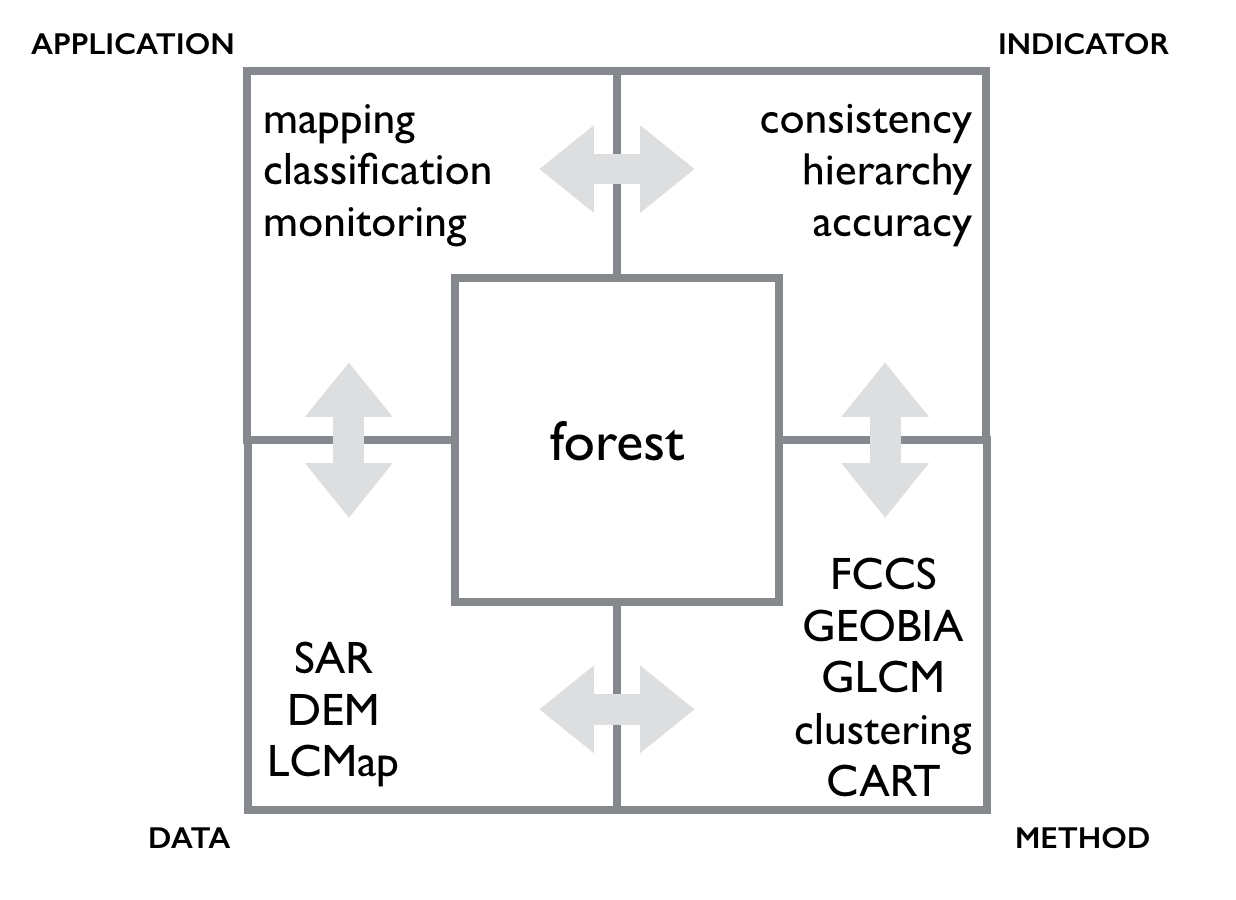
\includegraphics[width=1.0\textwidth]{fig_conceptual-framework.png}
	\caption[The conceptual framework of the study shows forest as the central theme enclosed by elements concerning data, method, indicator, and application, and their interrelationships.]{The conceptual framework of the study shows forest as the central theme enclosed by elements concerning data, method, indicator, and application, and their interrelationships.}
	\label{fig: litrev-fig2.5}
\end{figure}

\section{Aims and objectives}
\label{sec: litrev-aims-objectives}

Given the capabilities of ALOS/PALSAR data and above-mentioned image processing techniques, it is worth exploring their potentials for land and forest cover mapping in the Philippines. The general aim of this master’s research is to evaluate the suitability of ALOS/PALSAR mosaic data for mapping and monitoring of forest cover types in the Philippines based on the FAO forest cover classification system. To achieve this, the specific objectives of this thesis are as follows:

\begin{enumerate}
	\item To ascertain whether ALOS/PALSAR mosaic data are temporally consistent within a single acquisition year and across multiple acquisition years for the purpose of periodic monitoring;
	\item To establish a forest classification hierarchy based on the FAO forest classification system, and assess its consistency temporally and across feature attributes;
	\item To assess discrimination of forest cover types using ALOS/PALSAR mosaic data based on polarisation, topographic, and texture characteristics;
	\item To determine whether ancillary feature attributes (i.e., topographic, texture), in addition to polarisation, contribute to improving the classification accuracy of forest cover types; and
	\item To develop a hierarchical, stepwise classification approach for assessing the degree at which ALOS/PALSAR mosaic data can discriminate between forest cover types.
\end{enumerate}

\section{Scope and limitations}
\label{sec: litrev-scope-limitations}

Reference data used for this study, particularly as training and validation for the image classification, does not make use of ground-truth data. Rather, the study made use of the 2010 NAMRIA land cover map as the reference data. The official land cover map product was validated in the field by NAMRIA and fulfills acceptable classification accuracies (Raul Magabo, 2015, \textit{personal communication}), although documentation of the methods and accuracy assessment to accompany the map product has not yet been made publicly available. The multi-year ALOS/PALSAR mosaic data used in this study, which are different from the standard strip data product, were accessed through JAXA's Kyoto \& Carbon (K\&C) Initiative and were provided as is. The findings from this study may apply to the standard products, but may potentially differ unless the same pre- processing steps carried out on the mosaic data (Shimada \& Ohtaki, 2010) are similarly applied on the standard products.

	%--------------------------------------------------------------------------
% Methodology
%--------------------------------------------------------------------------

\chapter{Methodology}
\label{cha: methodology}

\section{Study area}
\label{sec: method-study-area}

The region of Northern Luzon, Philippines (approx. geographic coordinates: upper- left: 120$\,^{\circ}$ E, 18$\,^{\circ}$ N; lower-right: 123$\,^{\circ}$ E, 16$\,^{\circ}$ N) was chosen as an appropriate study area because all nine forest cover types based on the FAO FCCS were present in the region. The study area covers 16 provinces, either fully or partially, including: Abra, Apayao, Aurora, Benguet, Cagayan, Ifugao, Ilocos Norte, Ilocos Sur, Isabela, Kalinga, La Union, Mountain Province, Nueva Ecija, Nueva Vizcaya, Pangasinan, and Quirino (Fig. \ref{fig: method-fig3.1}). Northern Luzon experiences tropical cyclones very frequently, and spans three climate regimes based on the modified Coronas classification, particularly: Type I over Ilocos region (pronounced wet and dry season); Type III over Cagayan River Basin (short dry season with no pronounced maximum rain period); and Type IV over Northern Sierra Madre (no dry season and no pronounced maximum rain period).

The study area covers a total land area of 4.9 M ha, of which approximately 3.1 M ha (63\%) is comprised of non-forest land cover and 1.8M ha (37\%) is comprised of forest cover types based on the 2010 NAMRIA land cover map. Expansive agricultural areas are situated in the Cagayan Valley between the Cordilleras and Northern Sierra Madre ranges. Of the total land area of forest cover types, the majority is comprised of closed forest broadleaved (FCFB) at 38\%; open forest broadleaved (FOFB) at 46\%; open forest coniferous (FOFC) at 9\%; and the remaining 7\% by other forest cover types. A detailed tabulation of total land area of forest cover types per province is presented in Appendix 2.

\begin{figure}
	\centering
	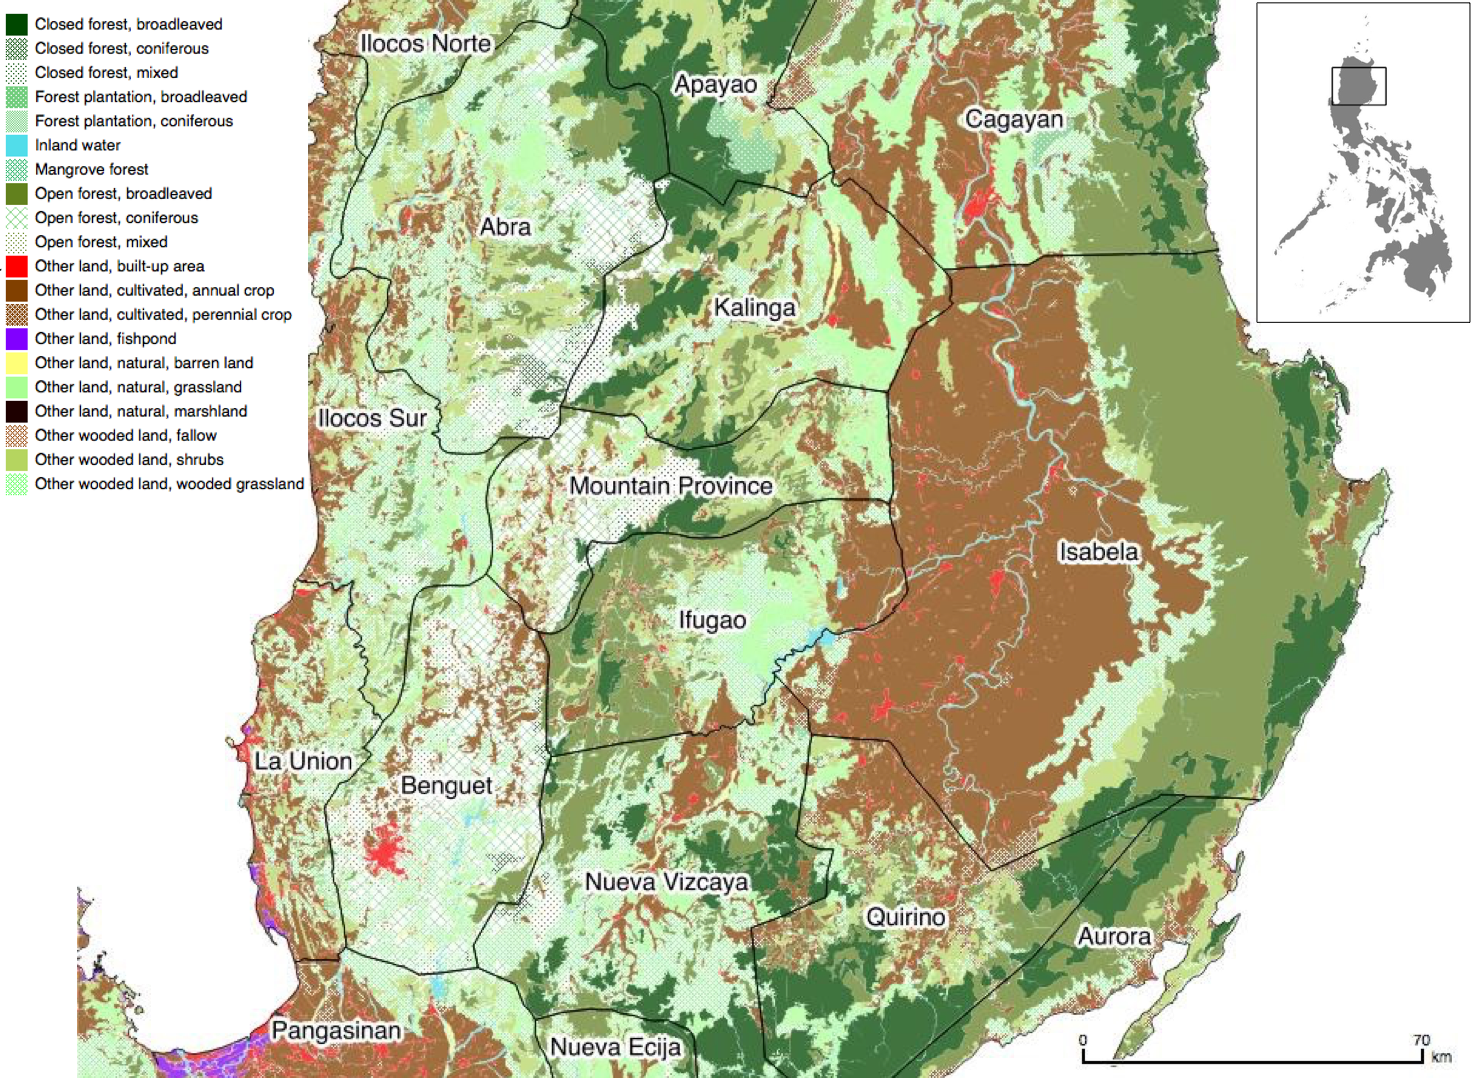
\includegraphics[width=1.0\textwidth]{fig_study-area.png}
	\caption[Study area in Northern Luzon, Philippines showing the 2010 land cover map based on NAMRIA data.]{Study area in Northern Luzon, Philippines showing the 2010 land cover map based on NAMRIA data.}
	\label{fig: method-fig3.1}
\end{figure}

\section{Data}
\label{sec: method-data}

For this study, the following datasets were used:

\begin{enumerate}
	\item Dual-polarised 25 m spatial resolution ALOS/PALSAR mosaic data (HH, HV) from JAXA through the K\&C Initiative (\cite{rosenqvist_initiating_2001}; \cite{rosenqvist_kyoto_2010}). The PALSAR mosaics, provided as 1x1 degree tiles, are radiometrically and geometrically calibrated large-scale datasets generated using JAXA's mosaicking algorithm, which consists of the pre-processing the long-strip PALSAR data; orthorectification and slope correction using a DEM; suppression of differences in intensity between neighbouring strips; and metadata preparation (e.g., dates of launch, local incidence angle, radar shadow, layover, and valid/invalid data) to support data interpretation (\cite{shimada_generating_2010}).
	Multi-year ALOS/PALSAR mosaic data (2007, 2008, 2009, 2010) were used to assess temporal consistency and suitability for periodic monitoring of forest cover. A total of 24 ALOS/PALSAR mosaic tiles were used with six tiles per year (i.e., 17N120E, 17N121E, 17N122E, 18N120E, 18N121E, 18N122E). All PALSAR tiles consist two channels, the HH and HV polarisation. The metadata layers, specifically the date of acquisition layer and the mask layer (for excluding radar shadow and layover pixels), corresponding to each mosaic tile per year were also used.
	\item Shuttle Radar Topography Mission (SRTM) elevation data product available from the United States Geological Survey. The SRTM DEM 1 arc-second (\url{~}30 m spatial resolution) global void-filled data was downloaded through the EarthExplorer portal. Nine DEM tiles were used (i.e., 16N120E, 16N121E, 16N122E, 17N120E, 17N121E, 17N122E, 18N120E, 18N121E, 18N122E).
	\item National 2010 NAMRIA land cover map. The data in vector format was accessed through the Forest Management Bureau. The land cover and forest type classes were based on the FAO GFRA categories (Table \ref{tab: intro-table2.1}) composed of a total of 20 land cover classes consisting of nine forest types.
\end{enumerate}

\section{Overall workflow}
\label{sec: method-overall-workflow}

The primary steps in the overall image processing workflow, which are discussed in the proceeding sub-sections, consists of image pre-processing (Sec. \ref{sec: method-preprocessing}), identification of regions of interest (Sec. \ref{sec: method-roi-identification}), image segmentation (Sec. \ref{sec: method-segmentation}), extraction of feature attributes and backscatter analysis (Sec. \ref{sec: method-feature-extraction}), hierarchical clustering (Sec. \ref{sec: method-clustering}), and decision tree classification and ruleset development (Sec. \ref{sec: method-decision-tree}). The overall workflow diagram shows the data used, intermediate outputs, processes implemented, and the final outputs (Fig. \ref{fig: method-fig3.2}).

\begin{figure}
	\centering
	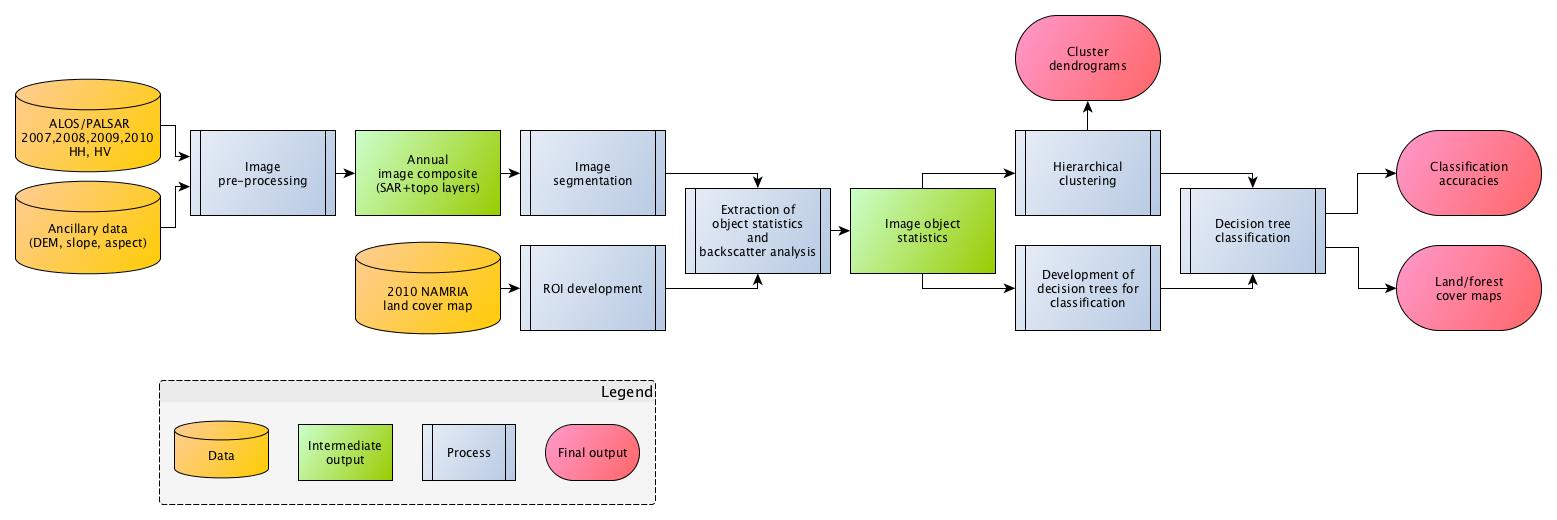
\includegraphics[width=1.0\textwidth]{fig_revised-methodology.jpg}
	\caption[Overall image processing workflow implemented in the study.]{Overall image processing workflow implemented in the study.}
	\label{fig: method-fig3.2}
\end{figure}

\section{Image pre-processing}
\label{sec: method-preprocessing}

Image pre-processing steps, which are presented as a sub-workflow diagram in Fig. \ref{fig: method-fig3.3}, were carried out in ENVI v.4.8 software (Exelis VIS, Inc. USA). For SAR data, each PALSAR data layer was mosaicked into a single regional image prior to geocoding and re-projection to UTM Zone 51 North coordinate system and WGS84 datum. The pixel dimensions of each image were 12844 columns x 8953 rows. To reduce signal noise from the radar data, a Lee filter was applied to preserve image sharpness and detail while suppressing speckle noise (\cite{lee_digital_1980}; \cite{lee_speckle_1981}), and with a small 5x5 kernel window to preserve texture information (\cite{lee_speckle_1994}). After minimising the speckles, ratio images (HH/HV) were generated using the HH and HV regional mosaics for each year. Then, HH and HV polarisation images were converted from amplitude to normalised radar cross-section, or sigma-nought ($\sigma$\textsuperscript{0}; units in dB) using Eq. \ref{eqn: method-eq1}:

\begin{equation} \label{eqn: method-eq1}
		\sigma^0=10\cdot log\textsubscript{10}[DN^2]+CF
\end{equation}

\noindent Where \textit{DN} is the digital number and \textit{CF} is the calibration factor with a value of –83.0 dB for ALOS/PALSAR data (\cite{rosenqvist_alos_2007}). A masking process was implemented on the PALSAR regional mosaics using the corresponding mask layers for each year to exclude unwanted pixels affected by shadow and layover in the radar data.

For the topographic data, the SRTM DEM tiles were mosaicked together prior to re- projection to UTM Zone 51 North WGS84, and subsequently resampled to 25 m spatial resolution and cropped to match the extents and dimensions of the SAR mosaic images. The slope and aspect layers were subsequently computed from the mosaicked DEM. Lower kernel sizes (i.e., 3x3, 5x5, and 7x7) were initially tested but the resulting models contained artifacts; hence, a 9x9 kernel size was used to generate the final slope (in percent) and aspect models.

\begin{figure}
	\centering
	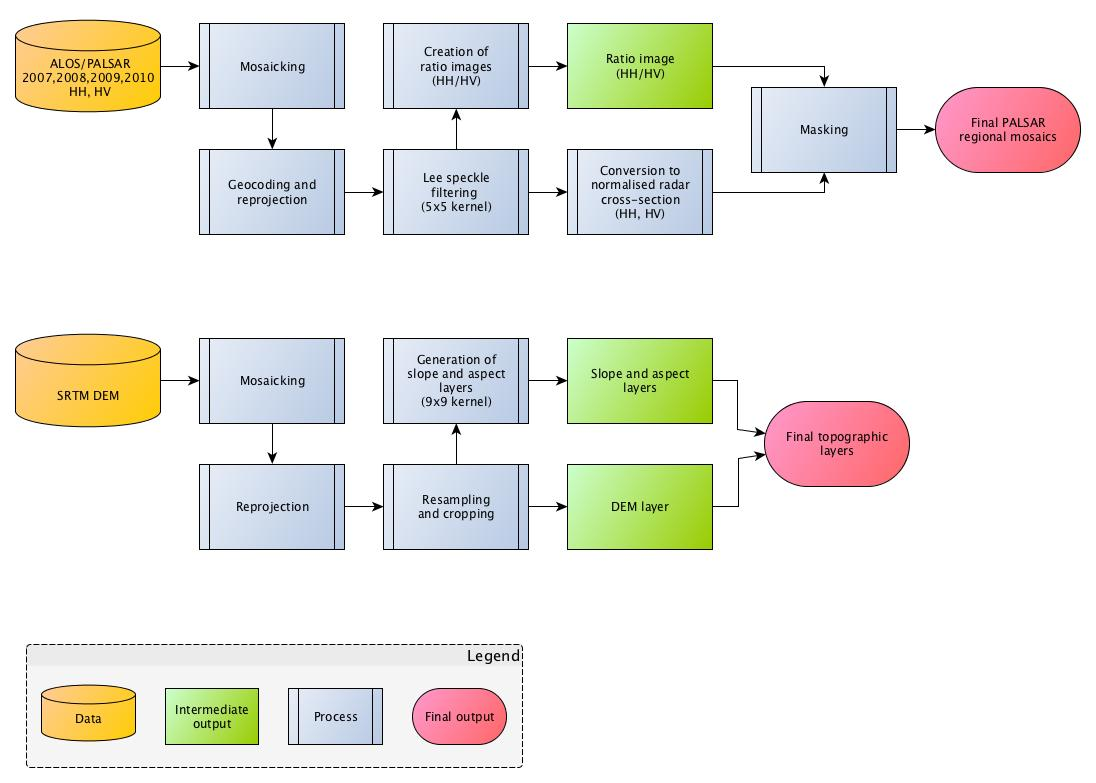
\includegraphics[width=1.0\textwidth]{fig_image-preprocessing.jpg}
	\caption[Detailed sub-workflow for image pre-processing steps implemented on SAR and topographic datasets.]{Detailed sub-workflow for image pre-processing steps implemented on SAR and topographic datasets.}
	\label{fig: method-fig3.3}
\end{figure}

\section{Design of a multi-level classification hierarchy}
\label{sec: method-class-hierarchy}

A multi-level land cover classification hierarchy was designed to guide the selection of regions of interest (ROI) and the decision tree classification (Fig. \ref{fig: method-fig3.4}). The first three levels were designed to classify the image into broad-level classes and extract the Forest class. Within the Forest class, after setting aside all Non-Forest class, the class hierarchy of subsequent levels was defined based on the result of the hierarchical clustering.

Starting with the entire image dataset, each level bifurcated into two classes and carried out sequentially one level after another. At Level 1, the data was split into either Land or Water classes. Then at Level 2, Water classes were set aside, and the Land class was assigned into either Vegetation or Non-Vegetation classes. At Level 3, the Vegetation class was split into either Forest or Non-Forest classes while the Non- Vegetation class was set aside. At Level 4, the splitting into forest types was carried out following the dendrograms resulting from the hierarchical cluster analysis.

\begin{figure}
	\centering
	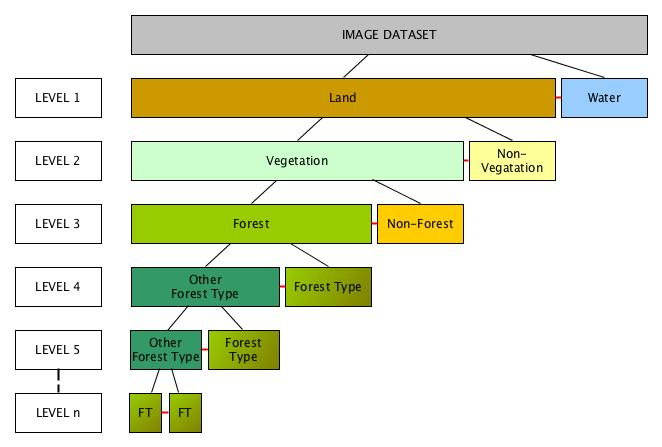
\includegraphics[width=1.0\textwidth]{fig_classification-hierarchy.jpg}
	\caption[The classification hierarchy proposed for this study.]{The classification hierarchy proposed for this study (note: FT is Forest Type).}
	\label{fig: method-fig3.4}
\end{figure}

\section{Identification of regions of interest}
\label{sec: method-roi-identification}

The identification of the ROIs was carried out in Quantum GIS v.2.12 software (QGIS Project Team). Prior to delineating ROIs, the detailed land cover classes were grouped into broad-level classes based on the multi-level classification hierarchy (Fig. \ref{fig: method-fig3.4}; Table \ref{tab: method-table3.1}). To aid in identifying and delineating the ROIs, the 2010 NAMRIA land cover map was used as a base map. The PALSAR mosaics were also visually inspected during the delineation of each ROI before assigning it to a specific class and to ensure a 5x5 kernel size polygon. Other ancillary vector data were also used to aid in identifying the ROIs, including OpenStreetMap data such as roads, buildings, and rivers (\cite{geofabrik_gmbh_philippines_2015}); and the Landsat-based 2010 mangrove map of the Philippines developed by Long et al. \citeyearpar{long_mapping_2013} to aid in identifying regions of interest in mangrove forests. A total of 1,451 ROIs were identified representing the land cover classes, and each ROI record reflected the multi-level classification hierarchy in the attribute table (Table \ref{tab: method-table3.1}). The distribution of the ROIs selected over the study area is shown in Fig. \ref{fig: method-fig3.5}.\\

\begin{spacing}{1.0}
\begin{longtable}[h!]{ p{1.4cm} p{1.8cm} p{1.4cm} p{6.9cm} p{1.5cm} }

    \caption[Hierarchy and grouping of land cover from detailed to broad-level classes.]{Hierarchy and grouping of detailed land cover classes into broad-level classes.}
    \label{tab: method-table3.1}\\
    
    	\toprule
    	Level 1 & Level 2 & Level 3 & 2010 NAMRIA Land Cover Classes & Number of ROIs\\ 
    	\midrule
    	\endhead
    	
		Land & Vegetation & Forest & Closed forest, broadleaved (FCFB) & 100\\
		{} & {} & {} & Closed forest, coniferous (FCFC) & 100\\
		{} & {} & {} & Closed forest, mixed (FCFM) & 100\\
		{} & {} & {} & Open forest, broadleaved (FOFB) & 186\\
		{} & {} & {} & Open forest, coniferous (FOFC) & 101\\
		{} & {} & {} & Open forest, mixed (FOFM) & 100\\
		{} & {} & {} & Forest plantation, broadleaved (FFPB) & 90\\
		{} & {} & {} & Forest plantation, coniferous (FFPC) & 30\\
		{} & {} & {} & Mangrove forest (LVMG) & 48\\[2pt]
		\cmidrule{3-5}
		{} & {} & Non- & Other wooded land, shrubs & 317\\
		{} & {} & Forest & Other wooded land, wooded grassland & {}\\
		{} & {} & {} & Other land, grassland & {}\\
		{} & {} & {} & Other land, annual crop & {}\\
		{} & {} & {} & Other land, perennial crop & {}\\[5pt]
		\cmidrule{2-5}
		{} & Non- & {} & Other wooded land, fallow & 67\\
		{} & Vegetation & {} & Other land, built-up area & {}\\
		{} & {} & {} & Other land, barren land & {}\\[5pt]
		\cmidrule{1-5}
		Water & {} & {} & Inland water & 212\\
		{} & {} & {} & Fishpond & {}\\
		\bottomrule
    
\end{longtable}
\end{spacing}

\begin{figure}
	\centering
	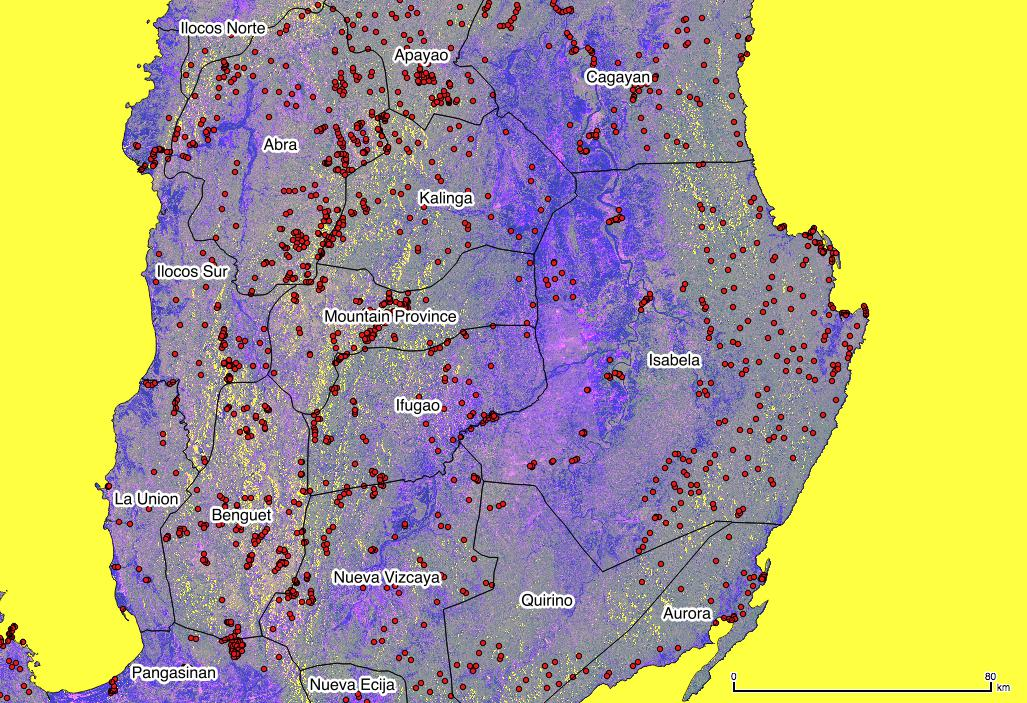
\includegraphics[width=1.0\textwidth]{fig_roi-locations.jpg}
	\caption[The distribution of the regions of interest selected over the study area in Northern Luzon, Philippines.]{The distribution of the regions of interest (red points) selected over the study area in Northern Luzon, Philippines. The 2010 PALSAR mosaic image is shown in the background.}
	\label{fig: method-fig3.5}
\end{figure}

\section{Image segmentation}
\label{sec: method-segmentation}

Image segmentation was implemented in eCognition Developer v.8.9 software (Trimble Germany GmbH). The segmentation method that is implemented in eCognition is an iterative process that minimises the average heterogeneity of generated segments (Baatz \& Schäpe, 2000). The measure of heterogeneity consists of a spectral and spatial component (Benz et al., 2004; Happ et al., 2010). Spectral heterogeneity is defined on the values of the spectral responses of the pixels within the segments. Spatial heterogeneity is based on two shape attributes: smoothness and compactness of the segments. Another parameter, scale, is the stopping criterion for the optimisation process. Prior to fusion of two adjacent objects, the resulting increase in heterogeneity is computed such that if the resulting increase exceeds a threshold determined by the scale parameter then no further fusion takes place and the segmentation stops (Benz et al., 2004). A merge with a better degree of fitting (i.e., smaller value) than the scale parameter fulfils the homogeneity criterion (Baatz \& Schäpe, 2000). Hence, the larger the scale parameter, the more objects can be fused and the larger the segments grow (Baatz \& Schäpe, 2000).

The input data for segmentation consisted of the set of images, including the 12 ALOS/PALSAR data layers (i.e., HH and HV polarisation and HH/HV ratio images for each year) and 3 topographic data layers (i.e, elevation, slope, and aspect), totalling 15 input image layers. To determine the values of the parameters to be used for image segmentation procedure, different values were tested on each parameter to see whether the resulting segments made an acceptable delineation of image features (Appendix 3.). For multi-resolution segmentation, the user sets the following parameters: scale, shape, compactness, and image weights. The values of 5, 10, and 20 were tested for the scale parameter. For shape and compactness, the values of 0.1, 0.5, and 0.9 were used for each parameter, thereby testing nine combinations of values between shape and compactness (i.e., 0.1-0.1; 0.1- 0.5; 0.1-0.9; 0.5-0.1; 0.5-0.5; 0.5-0.9; 0.9-0.1; 0.9-0.5; and 0.9-0.9). For image weights, a value of 1 was used uniformly on all layers, both for the SAR and topographic layers.

After a visual assessment of the segmentation tests, a scale parameter value of 10 was chosen since a value of 5 was too detailed and a value of 20 had generalised small features. Next, a shape value of 0.1 and a compactness value of 0.9 were selected since the segments closely followed the form of image features. For image weights, a value of 1 was retained for SAR data layers only. Topographic layers were given image weight values of 0 since they introduced regular-shaped rectangular segments that were not capturing the form of image features. The final values chosen for the multi-resolution segmentation parameters were: scale = 10; shape = 0.1; compactness = 0.9; image weights = 1 for SAR layers and 0 for topographic layers (Appendix 3). The total number of segments delineated for each PALSAR regional mosaic were as follows: 2007 = 182,876 segments; 2008 = 184,917 segments; 2009 = 186,369 segments; 2010 = 191,588 segments.

\section{Extraction of feature attributes and backscatter analysis}
\label{sec: method-feature-extraction}

Object-level feature attributes were computed for all the delineated land cover ROIs in eCognition software. Feature attributes were calculated, particularly the mean and standard deviation, both from the yearly PALSAR regional mosaics and topographic layers; and eight GLCM measures from each of the PALSAR data layers. The GLCM texture measures include angular second moment, contrast, correlation, dissimilarity, entropy, homogeneity, mean, and standard deviation (variance). Thirty feature attributes were extracted from the SAR data layers per year (including polarisation and texture attributes) and 6 attributes from the topographic layers (Table \ref{tab: method-table3.2}). Tabular databases were generated containing these feature attributes such that four tables were produced, each corresponding to the attributes per annual PALSAR regional mosaics plus the topographic layer attributes. These tabular databases were then used as inputs for subsequent backscatter analysis, the hierarchical clustering, and the decision tree classification in R statistical software (R Core Team, 2015).\\

\begin{spacing}{1.0}
\begin{longtable}[h!]{ p{2.6cm} p{2.6cm} p{2.6cm} p{2.6cm} p{2.6cm} }

    \caption[Object-level feature attributes extracted from the images.]{Object-level feature attributes extracted from the images.}
    \label{tab: method-table3.2}\\
    
    	\toprule
    	Polarisation & Topographic & {} & Texture & {}\\
    	\cmidrule{3-5}
    	{} & {} & GLCM HH & GLCM HV & GLCM HH/HV\\
    	\midrule
    	\endhead
    	
		Mean HH & Mean DEM & Ang. 2$^{nd}$ Mom & Ang. 2$^{nd}$ Mom & Ang. 2$^{nd}$ Mom\\
		Mean HV & Mean Slope & Contrast & Contrast & Contrast\\
		Mean HH/HV & Mean Aspect & Correlation & Correlation & Correlation\\
		SD HH & SD DEM & Dissimilarity & Dissimilarity & Dissimilarity\\
		SD HV & SD Slope & Entropy & Entropy & Entropy\\
		SD HH/HV & SD Aspect & Homogeneity & Homogeneity & Homogeneity\\
		{} & {} & Mean & Mean & Mean\\
		{} & {} & SD & SD & SD\\
		
		\bottomrule
    
\end{longtable}

	\noindent Note: HH, horizontal transmit - horizontal receive; HV, horizontal transmit - vertical receive; GLCM, grey level co-occurrence matrix; DEM, digital elevation model; SD, standard deviation.\\ \newline

\end{spacing}

PALSAR mosaic data are comprised of strip (or path) data acquired on different dates that are pre-processed and mosaicked together as end-user products (Fig. \ref{fig: intro-fig3.6}; Shimada \& Ohtaki, 2010). The strip data comprising one annual regional PALSAR mosaic were acquired over different seasons/dates. Also, the strip data along the same path acquired over the same locality were acquired over different years for the annual mosaics. To assess the temporal consistency of the PALSAR mosaic data, a radar backscatter analysis of forest cover types was done for PALSAR mosaics, first, across adjacent strips within a single acquisition year; and second, within the same strip across multiple acquisition years. Box-whisker plots were generated using the \textit{ggplot2} package in R software (Wickham \& Chang, 2015) to analyse the backscatter values of different forest types over the different dates of acquisition of the images.\\

\begin{figure}[!ht] \centering
	\captionsetup[subfigure]{width=2.0in} % <-- Use this to control text which is poorly spaced under a subfigure. 
	\begin{subfigure}[t]{0.49\textwidth}
		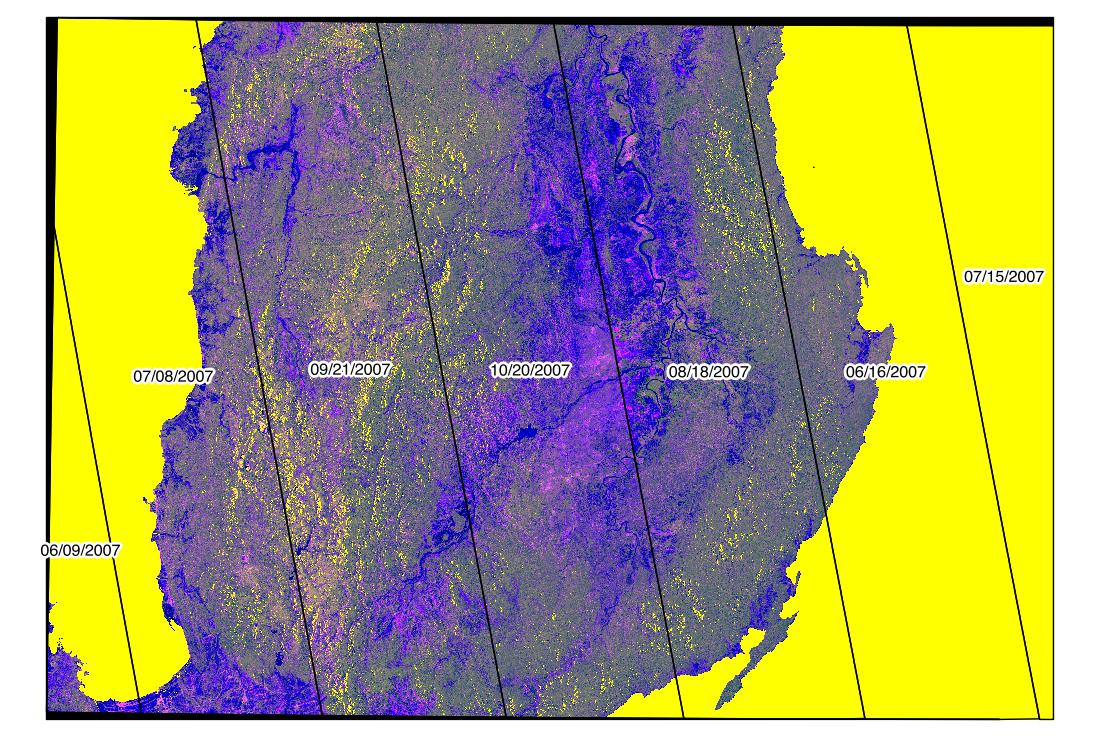
\includegraphics[width=\textwidth]{fig_palsar-2007-dates.jpg}
		\caption[Annual PALSAR mosaics.]{2007}
		\label{fig: method-fig3.6a}
	\end{subfigure}
	\begin{subfigure}[t]{0.49\textwidth}
		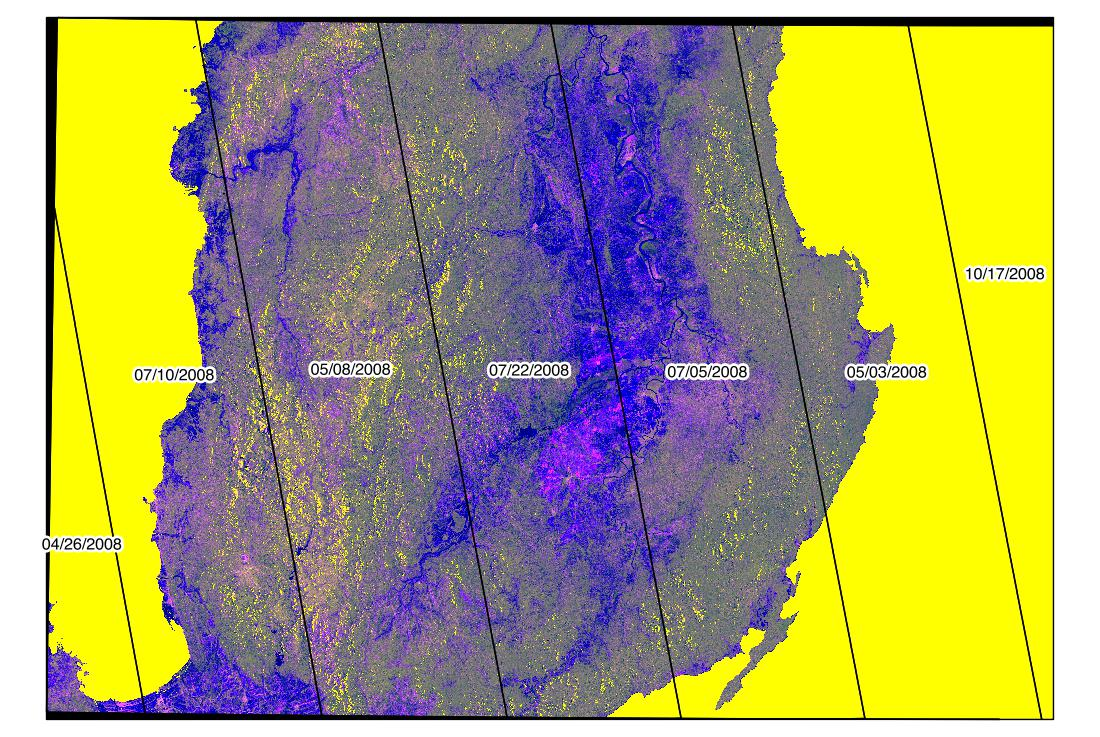
\includegraphics[width=\textwidth]{fig_palsar-2008-dates.jpg}
		\caption[Annual PALSAR mosaics.]{2008}
		\label{fig: method-fig3.6b}
	\end{subfigure}\\
	\vspace{10pt}
	\begin{subfigure}[t]{0.49\textwidth}
		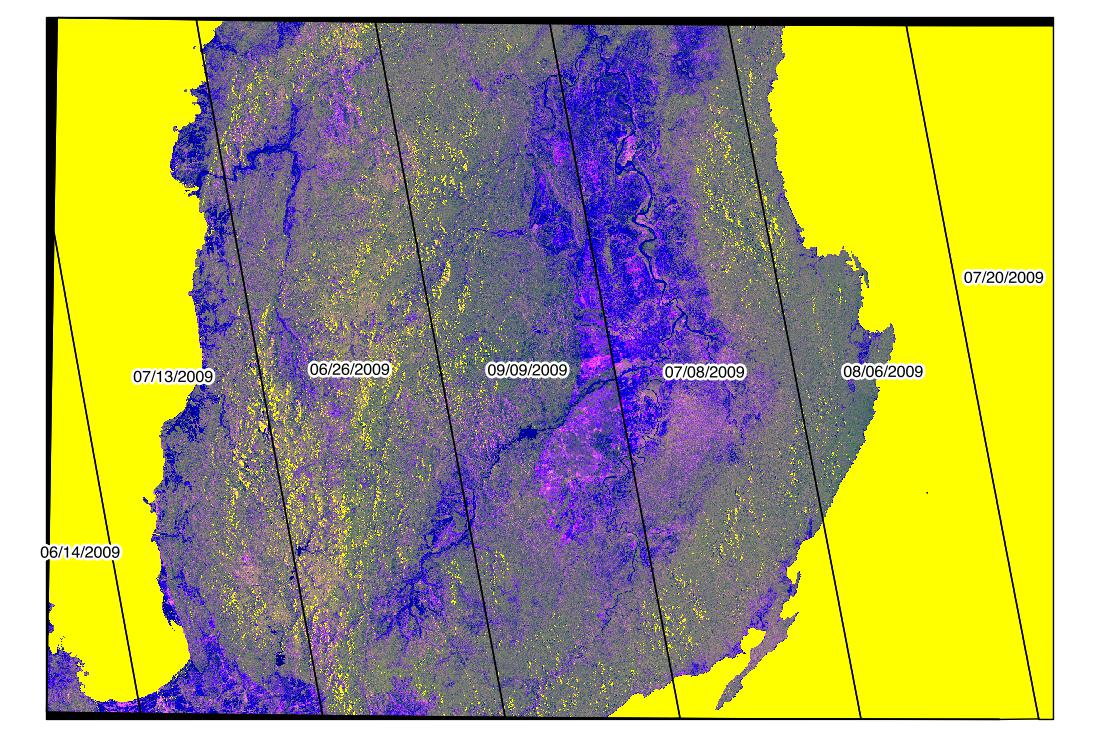
\includegraphics[width=\textwidth]{fig_palsar-2009-dates.jpg}
		\caption[Annual PALSAR mosaics.]{2009}
		\label{fig: method-fig3.6c}
	\end{subfigure}
	\begin{subfigure}[t]{0.49\textwidth}
		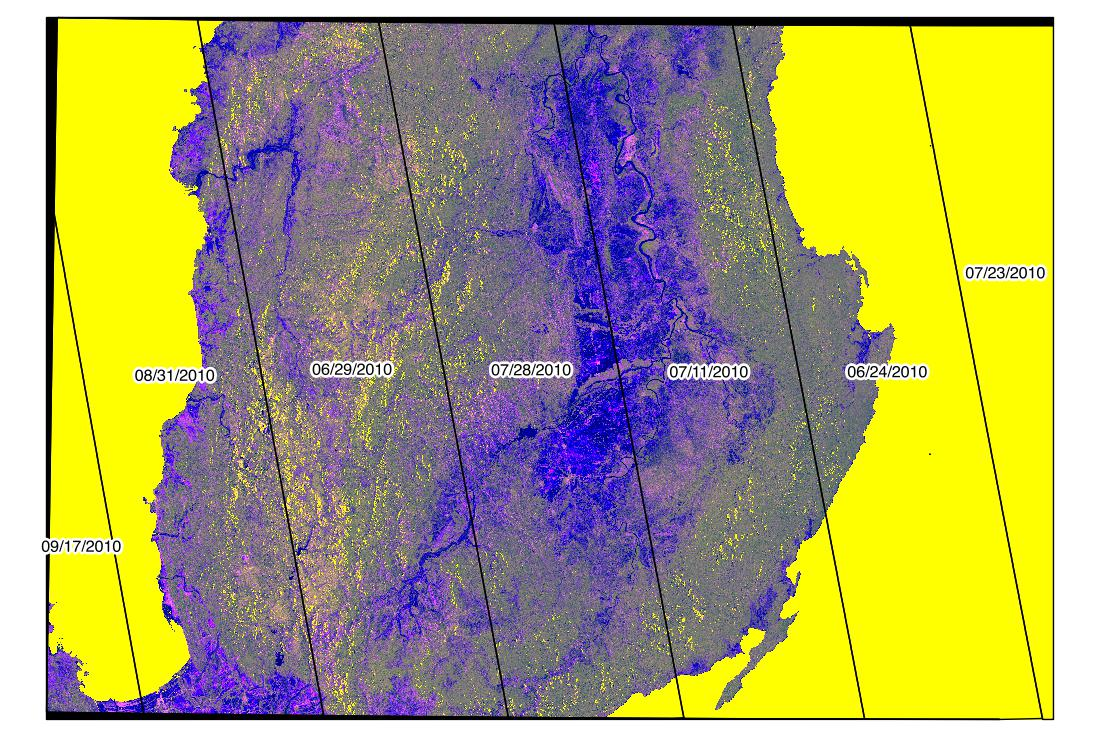
\includegraphics[width=\textwidth]{fig_palsar-2010-dates.jpg}
		\caption[Annual PALSAR mosaics.]{2010}
		\label{fig: method-fig3.6d}
	\end{subfigure}
	\caption[The annual PALSAR mosaics of Northern Luzon acquired in 2007, 2008, 2009, and 2010.]{The annual PALSAR mosaics of Northern Luzon acquired in (a) 2007, (b) 2008, (c) 2009, and (d) 2010. The extent of each strip (or path) data and the dates of acquisition of each strip are shown for each annual mosaic.}
	\label{fig: method-fig3.6}
\end{figure}

\section{Hierarchical clustering}
\label{sec: method-clustering}

Agglomerative hierarchical clustering was implemented using the \textit{pvclust} package in R software (Suzuki \& Shimodaira, 2006, 2014) with the tabular databases for each year as inputs. Both the temporal consistency of the multi-year SAR data and the cluster hierarchy of forest types were evaluated using the dendrograms. The \textit{pvclust} package was useful to assess the uncertainty or stability in hierarchical cluster analysis by calculating probability values (Suzuki \& Shimodaira, 2014). An approximately unbiased (AU) p-value $\geq$ 0.95 indicates consistent or stable clustering/grouping and is strongly supported by the data (Suzuki \& Shimodaira, 2014).\\

\begin{spacing}{1.0}
\begin{longtable}[h!]{ p{2cm} p{2cm} p{9cm} }

    \caption[Four cases representing combinations of object-level feature attributes.]{The four cases representing combinations of object-level feature attributes.}
    \label{tab: method-table3.3}\\
    
    	\toprule
    	Case & Number of variables & Combinations of object-level feature attributes\\
       	\midrule
    	\endhead
    	
		1 & 6 & Polarisation\\
		2 & 12 & Polarisation + Topographic\\
		3 & 30 & Polarisation + Texture\\
		4 & 36 & Polarisation + Topographic + Texture\\
		
		\bottomrule \\
    
\end{longtable}
\end{spacing}

Four cases representing combinations of object-level feature attributes were used in evaluating the temporal consistency of the cluster hierarchy of forest types (Table \ref{tab: method-table3.3}). Hierarchical clustering was applied across the four cases with each case involving the four annual PALSAR mosaics. For Case 1, only the Polarisation feature attributes were evaluated. For Case 2, the Polarisation and Topographic feature attributes were evaluated. For Case 3, the Polarisation and Texture feature attributes were evaluated. Finally, for Case 4, the all feature attributes were evaluated.

In any case, consistency of the cluster hierarchy means that the hierarchical structure of the dendrogram does not change and the order and location of the nodes represented by forest types do not vary. The consistency of dendrograms was assessed through pairwise comparisons of dendrograms, totalling six pairs in each case. Baker's Gamma Indices were computed using the \textit{dendextend} package in R software (Galili et al., 2015; Galili, 2015) for comparing clustering dendrograms. The Baker’s Gamma Index (referred to as $\beta$ coefficient from here on) is a measure of association (similarity) between two dendrograms of hierarchical clustering (Baker, 1974). It is defined as a rank correlation between the stages at which pairs of objects combine in each of the two dendrograms (Fowlkes \& Mallows, 1983). A Spearman's correlation is computed and the values can range between -1 to 1 with near 0 values meaning that the two dendrograms are not statistically similar (Galili et al., 2015). The Baker's Gamma Indices for pairwise comparison of dendrograms for all cases were summarised and ranked to determine which case (or combination of feature attributes) gave the higher similarity between dendrograms.

\section{Decision tree classification and ruleset development}
\label{sec: method-decision-tree}

A decision tree classification approach using the \textit{tree} package in R software (Ripley, 2015), which is based on the CART algorithm by Breiman et al. (1984), was used to construct decision tree models. The tabular databases were used as the inputs for decision tree classification, designating the feature attributes as predictor variables and assigning classes depending on the classification level. At Level 1 classification, all objects were assigned into either Land or Water classes. Then at Level 2, Water classes were set aside, and only objects classified as Land from Level 1 were subsequently assigned into either Vegetation or Non-Vegetation classes. At Level 3, only objects classified as Vegetation from Level 2 are assigned into either Forest or Non-Forest classes while setting aside Non-Vegetation classes. In subsequent classification levels, forest cover types were classified one by one based the results of the hierarchical clustering until all forest cover types were classified.

Decision tree models were developed based on four cases or combinations of feature attributes to determine whether ancillary feature attributes (i.e., topographic, texture), in addition to polarisation, contribute to improving the classification accuracy of forest cover types. All decision trees were pruned using k-fold cross-validation to prevent overfitting. The case yielding the lowest misclassification error rates was selected and used as the basis for generating classification trees for each level for each year. A total of 44 classification trees were generated consisting of 11 trees in each year. The decision tree models produced in R software were translated as the bases for constructing the multi-level classification rulesets to produce forest cover maps in eCognition software.

An additional assessment of classification accuracies was done to discriminate closed and open canopy forests without following the hierarchical clustering result. The first three classification levels were maintained. At Level 4, mangrove forest (LVMG) was separated from all other forest types. For the final classification at Level 5, closed and open canopy forests were separated. Closed canopy forests included: closed broadleaved (FCFB), closed coniferous (FCFC), and closed mixed (FCFM). Open canopy forests included: open broadleaved (FOFB), open coniferous (FOFC), open mixed (FOFM), broadleaved forest plantation (FFPB), and coniferous forest plantation (FFPC).

	%--------------------------------------------------------------------------
% Results
%--------------------------------------------------------------------------

\chapter{Results}
\label{cha: results}

\section{Temporal consistency of PALSAR mosaic data}
\label{sec: result-temporal-consistency}

Two sets of figures were used for analysing the distribution of radar backscatter vis-a-vis data acquisition dates. The first set consists of PALSAR mosaic data that were acquired in a single year but the data strips used to put the mosaic together were taken at different seasons; and the second consists of PALSAR mosaic data acquired along the same data strip or path but at different years.

\subsection{Mosaic data acquired in a single year but at different seasons}

Figs. \ref{fig: result-box4.1} and \ref{fig: result-box4.2} shows the distribution of backscatter values of forest cover types from PALSAR mosaic data acquired in a single year but at different seasons. The backscatter values of different forest types were plotted with respect to polarisation. Each mosaic is comprised of six strip data paths, particularly where there is land.

As an example, the figures in Fig. \ref{box: result-box4.3} show the 2007 PALSAR mosaic image and the dates of acquisition of each strip/path that comprise the whole mosaic (top), and the distribution of mean HH polarisation backscatter of each forest type based on the ROIs on the 2007 mosaic image (bottom). The images were taken from Fig. \ref{fig: method-fig3.6} and Figs. \ref{fig: result-box4.1} and \ref{fig: result-box4.2}, respectively. In the mosaic image, the dates of acquisition of the strips from left to right were taken at different months of the year, specifically: Jun 09, Jul 08, Sep 21, Oct 20, and Jun 16. Then, for the boxplots, the mean HH backscatter (y-axis) was plotted from the ROIs of each of the different forest cover types (x-axis), and under each forest cover type there can be a number of boxplots where each colour denotes the date of acquisition of the corresponding PALSAR strip data. For each box-whisker plot, the upper and lower hinges of the box correspond to the 1st and 3rd quartiles (25th and 75th percentiles). The band inside the box corresponds to the median (or the 2nd quartile). The upper whisker extends from the hinge to the highest value that is within 1.5 x IQR of the hinge, where IQR is the inter-quartile range, or distance between the 1st and 3rd quartiles. The lower whisker extends from the hinge to the lowest value within 1.5 x IQR of the hinge. Data beyond the end of the whiskers are outliers and are plotted as points.

The range of mean HH backscatter values fell between -2.50 dB and -11.25 dB across all forest cover types. It can be seen that for broadleaved forests, including closed and open canopy and forest plantation (FCFB, FOFB, FFPB), the mean HH backscatter values were recorded over four data strips/paths. Forest cover types with ROI samples recorded in three data strips/paths include open canopy coniferous forest (FOFC) and open canopy mixed forest (FOFM). The other forest types were distributed along only two data strips/paths, particularly: closed canopy coniferous forest (FCFC), closed canopy mixed forest (FCFM), and mangrove forest (LVMG), of which mangroves were only found along strip path data over coastlines. It should be noted that ROI samples for mangrove forest along the far left data strip/path (i.e., Jun 09) were not sufficient for plotting, hence the box-whisker plot was truncated. And finally, the coniferous forest plantation (FCFP) was recorded only within one data strip/path (i.e., Sep 21).

For FCFB, the ranges of mean backscatter values as shown by the boxplots generally overlapped (i.e., Jun 16, Aug 18, Sep 21), and hence can be considered temporally consistent, although the Oct 20 boxplot was slightly greater than the other plots. For FCFC and FCFM, boxplots denoting two adjacent data strips (i.e., Sep 21, Oct 20) also overlapped; hence their mean backscatter values can be treated as temporally consistent. For FFPB, three boxplots overlapped (i.e., Jul 08, Sep 21, Oct 20), which denote that their mean backscatter values can be considered temporally consistent. The Aug 18 boxplot shows lower mean backscatter, which can be attributed to low backscatter returning to the antenna due to karst substrate (i.e., Peñablanca Protected Landscape in Tuguegarao, Cagayan province) upon checking the locations of the ROIs found along the data strip. For FFPC, mean backscatter values were recorded on only one data strip (i.e., Sep 21). For FOFB, FOFC, and FOFM, all boxplots overlapped, indicating that mean backscatter values acquired over different months were within the same range, and hence were temporally consistent. For LVMG, the two boxplots overlapped (i.e., Jun 16, Aug 18), and hence their mean backscatter values can be considered as temporally consistent. Overall, the general overlaps shown by boxplots of each forest cover type suggest that the range of mean HH backscatter values over PALSAR mosaic data strips acquired in different months can be treated as temporally consistent.

Now looking at Figs. \ref{fig: result-box4.1} and \ref{fig: result-box4.2}, three plots are shown for each of the four years (hence, a total of 12 plots) that correspond to boxplots of mean HH backscatter, mean HV backscatter, and HH/HV ratio across the different forest cover types.

The mean HH backscatter of most forest types across four years (2007-2010) was approximately between -2.50 dB to -11.25 dB in terms of their minimum and maximum values, indicating values were generally consistent across different seasons. For mangrove forest (LVMG), the backscatter values were approximately below -5.0 dB. Broadleaved forests, both closed and open canopy (FCFB, FOFB), exhibited narrow ranges denoting lower variability, and their median values were also generally consistent at the same level and did not vary across different seasons or different years.

The mean HV backscatter of most forest types across four years was approximately between -7.50 dB to -17.50 dB in terms of their minimum and maximum values, also indicating that values were generally consistent across different seasons within mosaic image acquired within a single year. Mangrove forest (LVMG) backscatter values were approximately between -11.0 dB and -17.5 dB, and generally had lower backscatter values compared to other forest cover types (notably the 25th to 75th percentile range of boxplots). Similar to mean HH backscatter, broadleaved forests, both closed and open canopy (FCFB, FOFB), also exhibited narrow ranges denoting lower variability, and their median values were also generally consistent at the same level and did not vary across different seasons or different years.

For the mean HH/HV ratio plots, values were approximately from 1.5 to 2.5 for all forest types (excluding outliers). Mangrove forest (LVMG) exhibited higher median values, generally observed at 2.0 and above, compared to other forest types that had values from 1.5 to 2.0.

\subsection{Mosaic data acquired along one path of strip data but across different years}

Figure 13 shows the distribution of backscatter values of forest cover types from PALSAR mosaic data from only one path of strip data but across different years. Similar to Figure 12, the backscatter values of different forest types were also plotted with respect to polarisation, and each mosaic is comprised of six strip data paths, particularly where there is land.

As an example, the figures in Fig. \ref{box: result-box4.4} show the one of the PALSAR regional mosaics with a highlight along the specific strip/path where ROIs of forest cover types were taken across different years, specifically from 2007 to 2010 (top), and the distribution of mean HH polarisation backscatter of each forest type along the same strip/path at different years (bottom). The images were taken from Fig. \ref{fig: method-fig3.6} and Figure 13, respectively. The dates of acquisition along the same strip/path taken at different years were: 21 Sep 2007, 08 May 2008, 26 Jun 2009, and 29 Jun 2010. Then, for the boxplots, the mean HH backscatter (y-axis) was plotted from the ROIs of each of the different forest cover types (x-axis), except for mangrove forest (LVMG) since there were no mangroves present within the data strip. Under each forest cover type there can be a number of boxplots where each colour denotes the date of acquisition along the same strip at different years.

The range of mean HH backscatter values fell between -2.50 dB and -11.25 dB across all forest cover types across different years. Median values of mean HH backscatter at different years consistently overlapped for each forest cover type, except for some very slight fluctuations. Overall, the overlaps shown by boxplots of each forest cover type suggest that the range of mean HH backscatter values over the same PALSAR mosaic data strip acquired in different years can be considered as temporally consistent.

Now looking at Figure 13, three plots are shown for each of the two highlighted data strips/paths that correspond to boxplots of mean HH backscatter, mean HV backscatter, and HH/HV ratio across the different forest cover types. Backscatter values were assessed for two different data strips/paths: one in Cordillera (Strip 1) and the other in Sierra Madre (Strip 2). Eight forest types were present along the Cordillera strip (except mangrove forest) while four forest types were present in the Sierra Madre strip (except coniferous and mixed forest types).

For the Cordillera data strip (Strip 1), the mean HH backscatter values were approximately from -2.5 dB to -10.0 dB, while the mean HV backscatter values were approximately from -7.5 dB to -15.0 dB. Median values were at consistent levels across different years for each forest type. The mean HH/HV ratio values were generally from 1.0 to 2.0 with consistent median values across different years for each forest type. For the Sierra Madre data strip (Strip 2), the mean HH backscatter values were approximately from -5.0 dB to -10.0 dB, while the mean HV backscatter values were approximately from -10.0 dB to -17.5 dB, of which mangrove forest (LVMG) had lower values compared to broadleaved forest types. Median values were generally at consistent levels across different years for each forest type. The mean HH/HV ratio values were also generally from 1.0 to 2.0, except for mangrove forest with values of 2.0 and above.

Overall, the distribution of mean backscatter of forest cover types for both HH and HV polarisation overlapped. The values of forest cover types in HH/HV ratio also overlapped, except for mangrove forest (LVMG), which had slightly higher values compared to other forest types. This emphasises that these forest types cannot be discriminated using solely polarimetric data.

The backscatter analysis demonstrated that the ALOS/PALSAR mosaics were temporally consistent despite the difference in seasons of acquisition dates of the strip data (usually within a range of 3-5 months) or the difference in annual dates of acquisition.

\begin{landscape}
\begin{figure}[!ht] \centering
	\captionsetup[subfigure]{width=2.0in} % <-- Use this to control text which is poorly spaced under a subfigure. 
	\begin{subfigure}[t]{0.43\textwidth}
		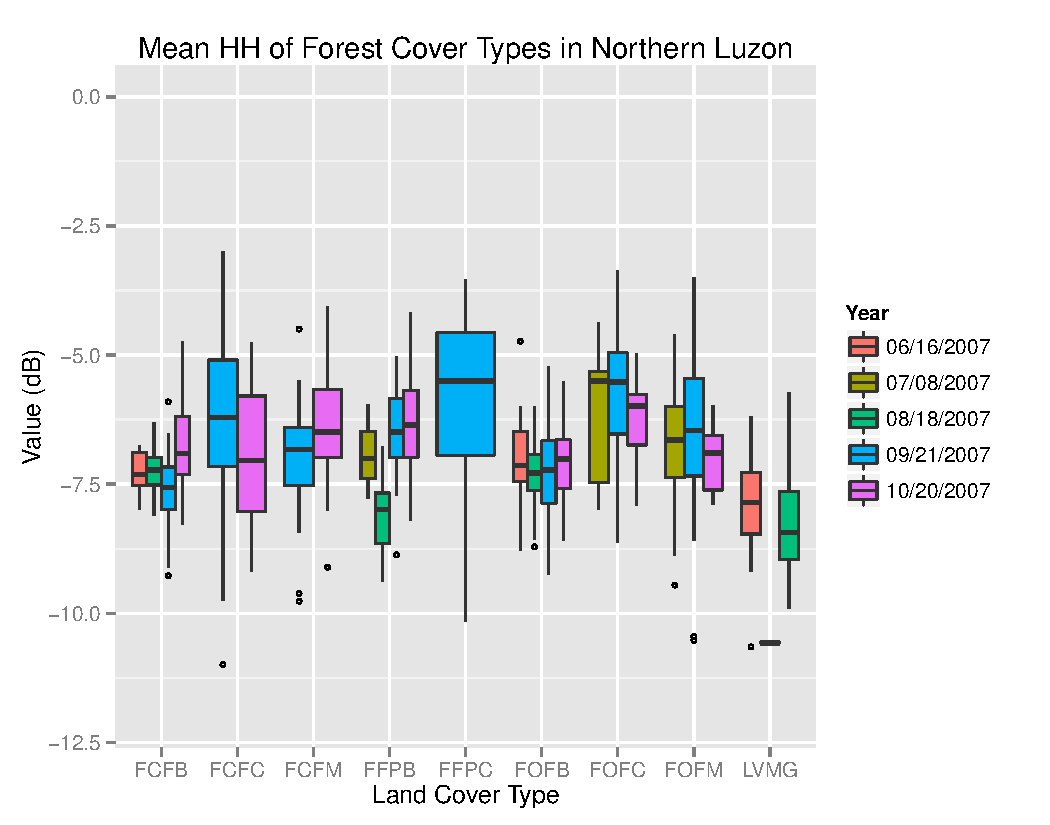
\includegraphics[width=\textwidth]{fig_boxplot-2007-mean-hh.pdf}
		\caption[Single year backscatter boxplots.]{2007 Mean HH.}
		\label{fig: result-box4.1a}
	\end{subfigure}
	\begin{subfigure}[t]{0.43\textwidth}
		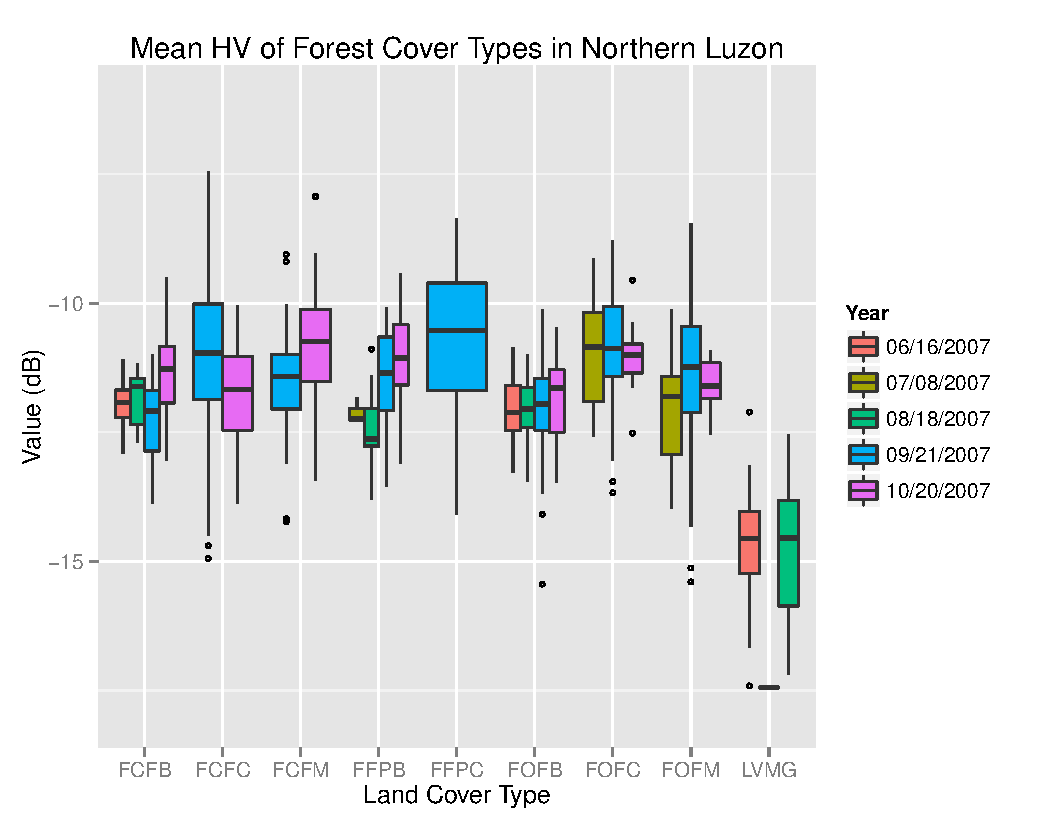
\includegraphics[width=\textwidth]{fig_boxplot-2007-mean-hv.pdf}
		\caption[Single year backscatter boxplots.]{2007 Mean HV.}
		\label{fig: result-box4.1b}
	\end{subfigure}
	\begin{subfigure}[t]{0.43\textwidth}
		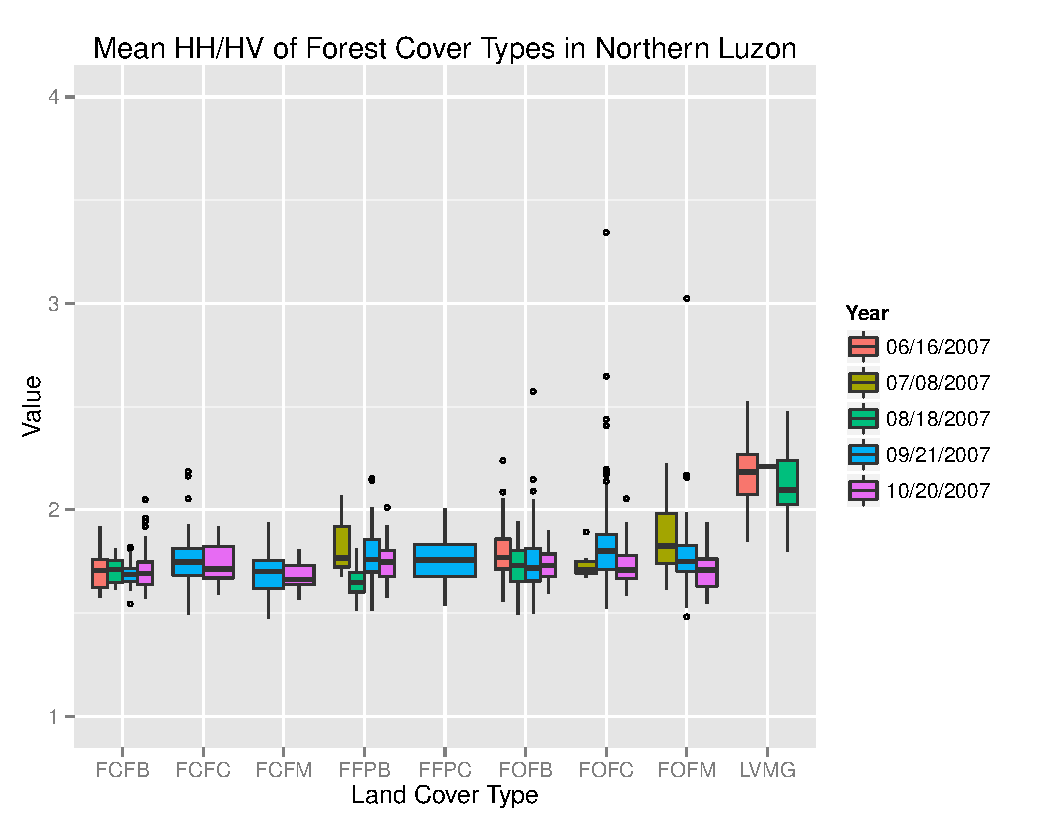
\includegraphics[width=\textwidth]{fig_boxplot-2007-mean-rat.pdf}
		\caption[Single year backscatter boxplots.]{2007 Mean HH/HV.}
		\label{fig: result-box4.1c}
	\end{subfigure}\\
	\vspace{20pt}
	\begin{subfigure}[t]{0.43\textwidth}
		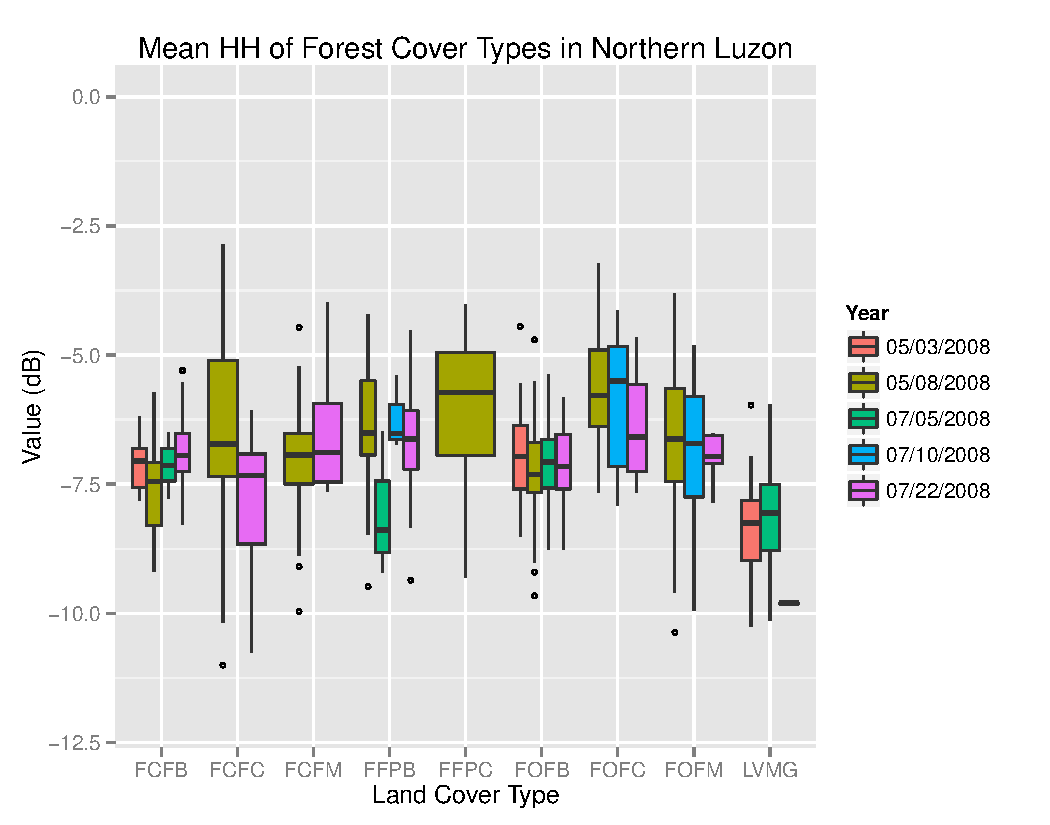
\includegraphics[width=\textwidth]{fig_boxplot-2008-mean-hh.pdf}
		\caption[Single year backscatter boxplots.]{2008 Mean HH.}
		\label{fig: result-box4.1d}
	\end{subfigure}
	\begin{subfigure}[t]{0.43\textwidth}
		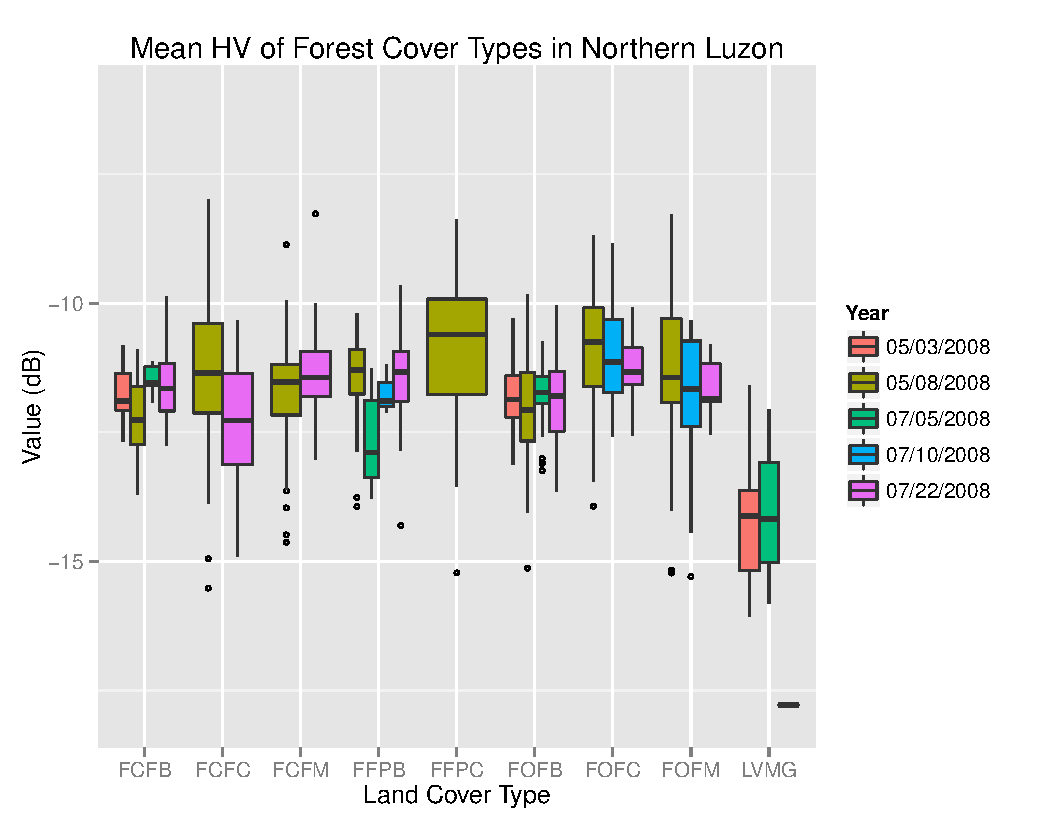
\includegraphics[width=\textwidth]{fig_boxplot-2008-mean-hv.pdf}
		\caption[Single year backscatter boxplots.]{2008 Mean HV.}
		\label{fig: result-box4.1e}
	\end{subfigure}
	\begin{subfigure}[t]{0.43\textwidth}
		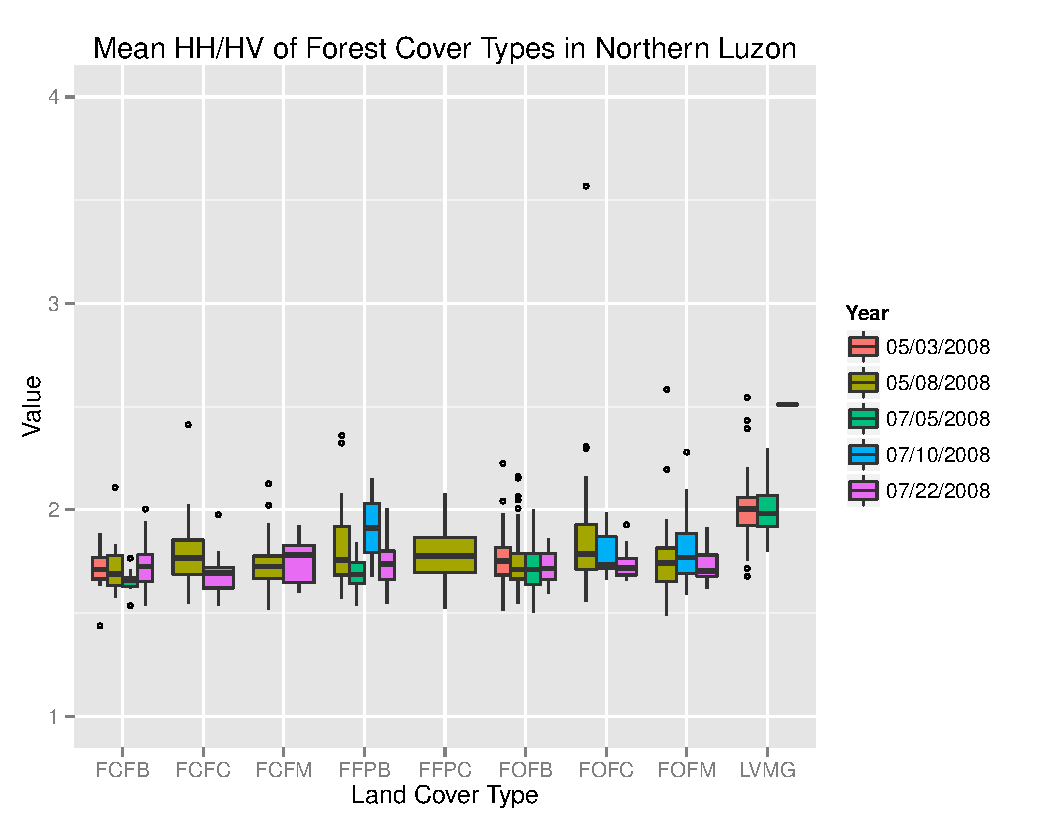
\includegraphics[width=\textwidth]{fig_boxplot-2008-mean-rat.pdf}
		\caption[Single year backscatter boxplots.]{2008 Mean HH/HV.}
		\label{fig: result-box4.1f}
	\end{subfigure}\\
	\vspace{20pt}
	\caption[Backscatter values of forest types from PALSAR data acquired in a single year at different seasons.]{Backscatter values of forest types from PALSAR data acquired in a single year at different seasons. Shown are box-whisker plots of mean backscatter values in 2007 (a-c) and 2008 (d-f).}
	\label{fig: result-box4.1}
\end{figure}
\end{landscape}

\begin{landscape}
\begin{figure}[!ht] \centering
	\captionsetup[subfigure]{width=2.0in} % <-- Use this to control text which is poorly spaced under a subfigure. 
	\begin{subfigure}[t]{0.43\textwidth}
		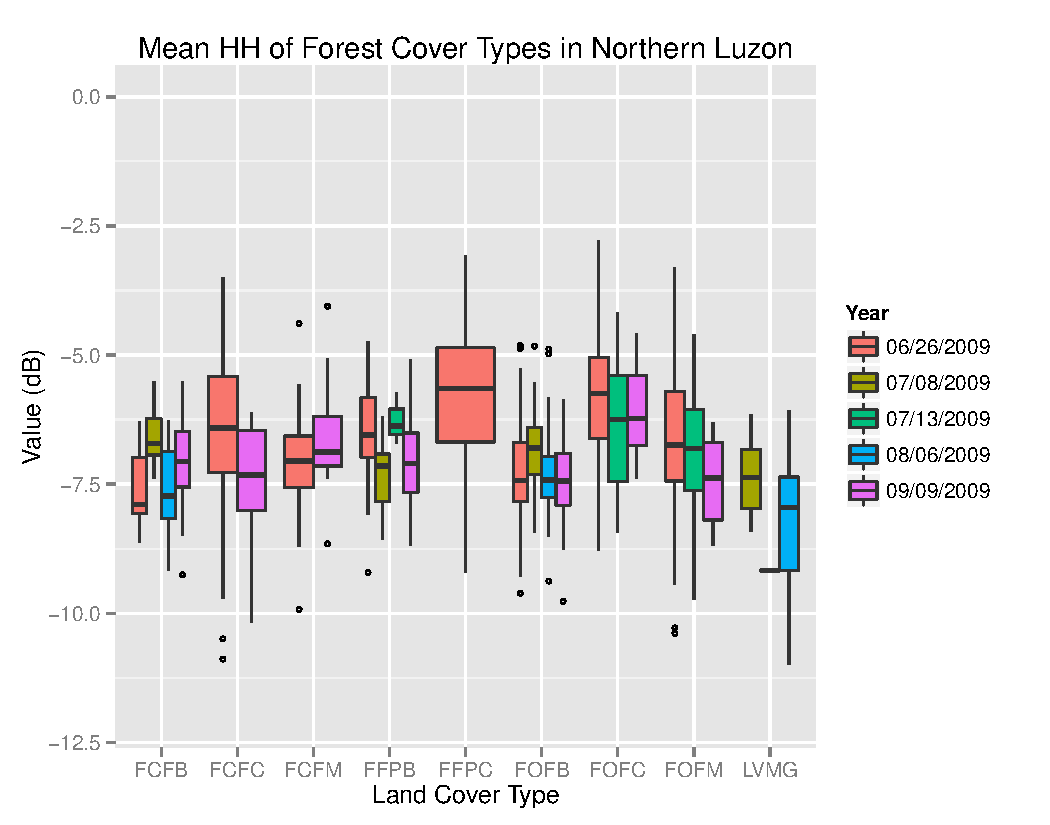
\includegraphics[width=\textwidth]{fig_boxplot-2009-mean-hh.pdf}
		\caption[Single year backscatter boxplots.]{2009 Mean HH.}
		\label{fig: result-box4.2a}
	\end{subfigure}
	\begin{subfigure}[t]{0.43\textwidth}
		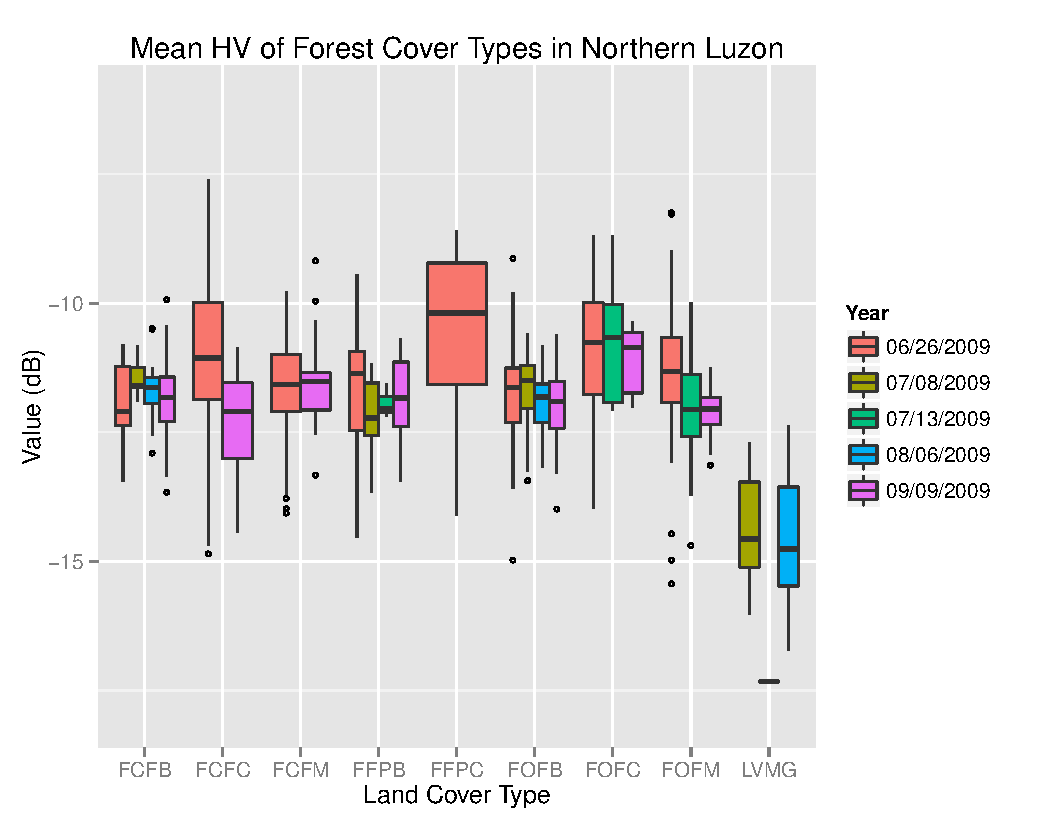
\includegraphics[width=\textwidth]{fig_boxplot-2009-mean-hv.pdf}
		\caption[Single year backscatter boxplots.]{2009 Mean HV.}
		\label{fig: result-box4.2b}
	\end{subfigure}
	\begin{subfigure}[t]{0.43\textwidth}
		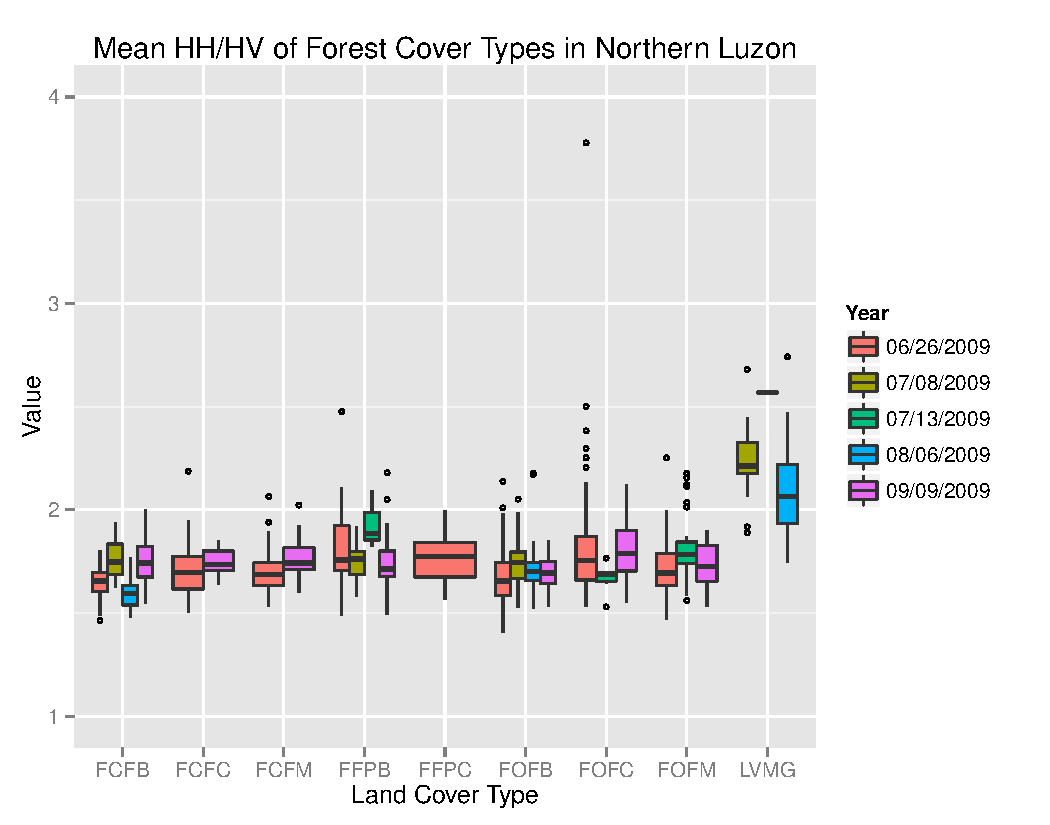
\includegraphics[width=\textwidth]{fig_boxplot-2009-mean-rat.pdf}
		\caption[Single year backscatter boxplots.]{2009 Mean HH/HV.}
		\label{fig: result-box4.2c}
	\end{subfigure}\\
	\vspace{20pt}
	\begin{subfigure}[t]{0.43\textwidth}
		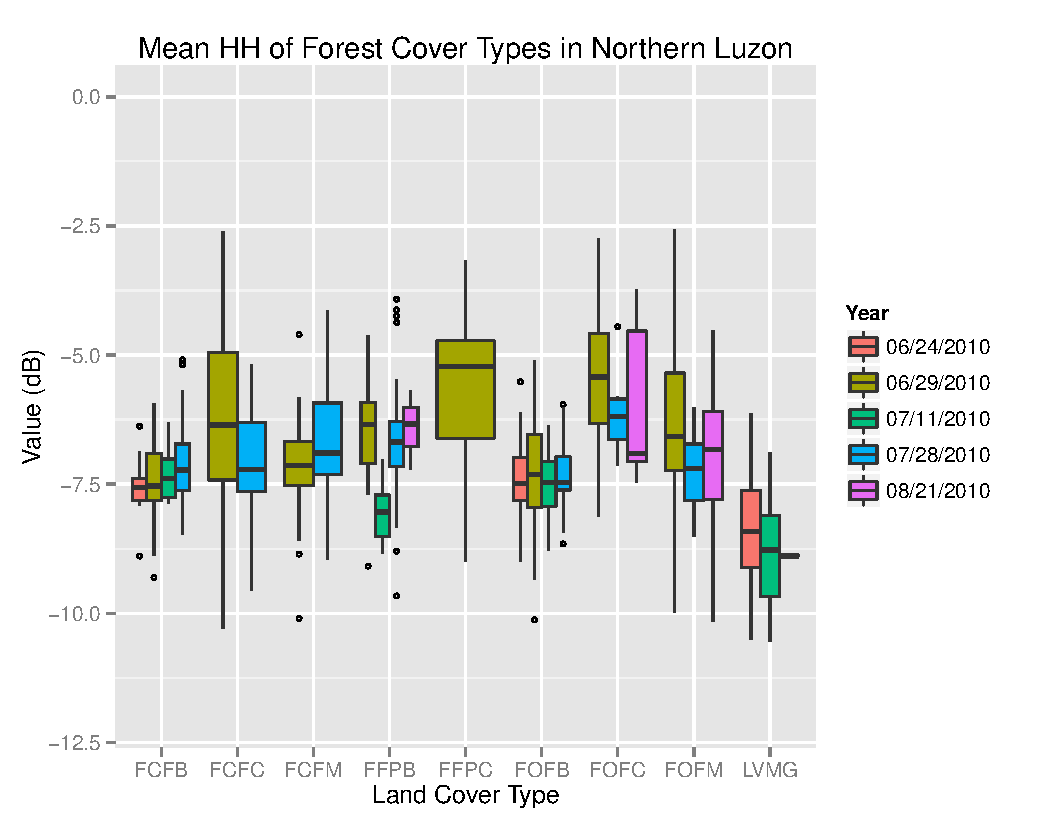
\includegraphics[width=\textwidth]{fig_boxplot-2010-mean-hh.pdf}
		\caption[Single year backscatter boxplots.]{2010 Mean HH.}
		\label{fig: result-box4.2d}
	\end{subfigure}
	\begin{subfigure}[t]{0.43\textwidth}
		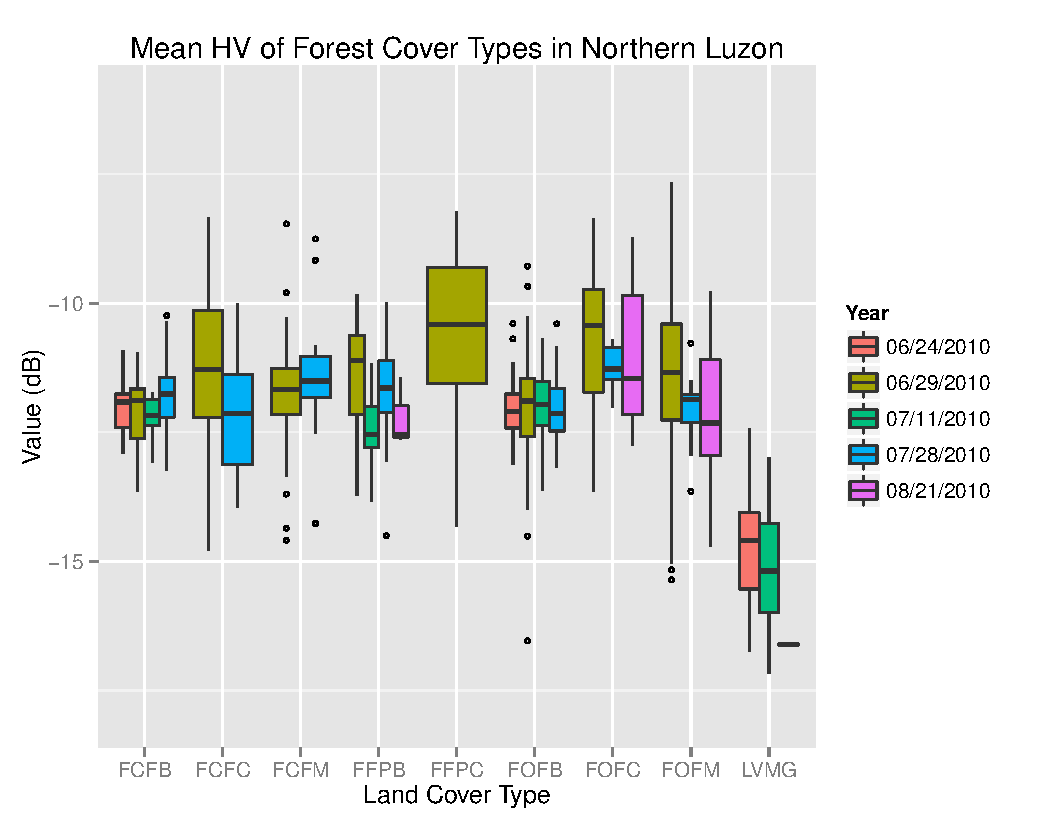
\includegraphics[width=\textwidth]{fig_boxplot-2010-mean-hv.pdf}
		\caption[Single year backscatter boxplots.]{2010 Mean HV.}
		\label{fig: result-box4.2e}
	\end{subfigure}
	\begin{subfigure}[t]{0.43\textwidth}
		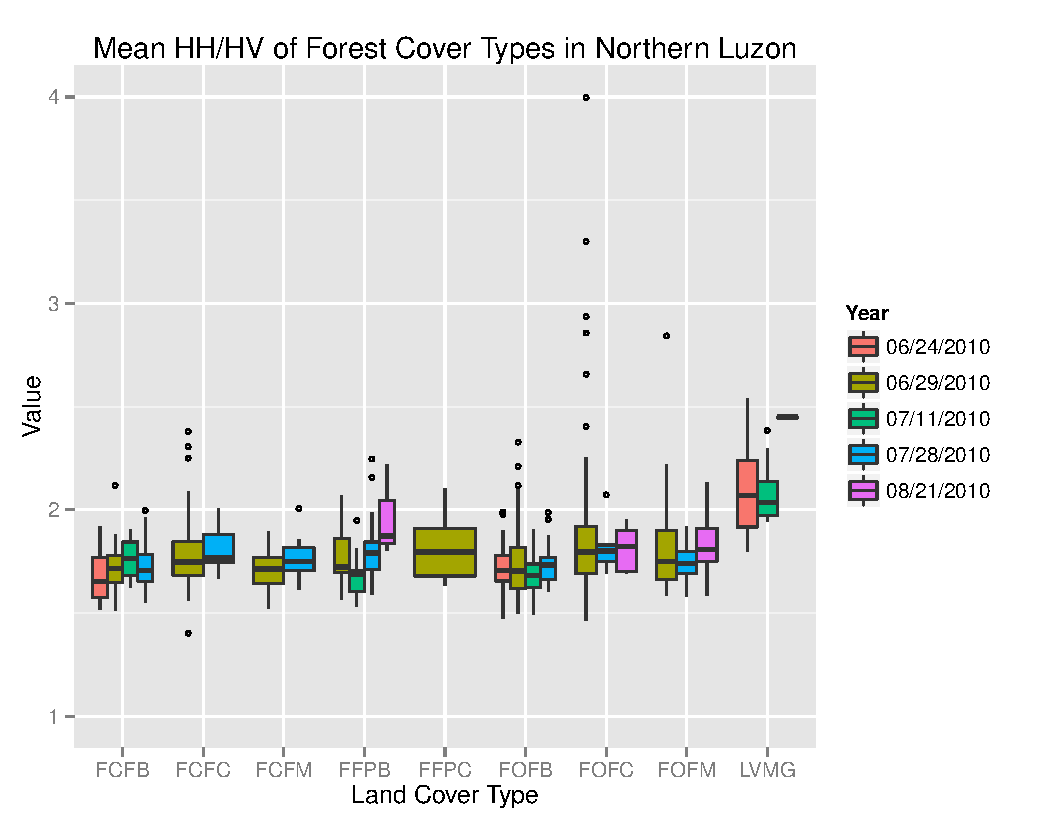
\includegraphics[width=\textwidth]{fig_boxplot-2010-mean-rat.pdf}
		\caption[Single year backscatter boxplots.]{2010 Mean HH/HV.}
		\label{fig: result-box4.2f}
	\end{subfigure}\\
	\vspace{20pt}
	\caption[Backscatter values of forest types from PALSAR data acquired in a single year at different seasons.]{Backscatter values of forest types from PALSAR data acquired in a single year at different seasons. Shown are box-whisker plots of mean backscatter values in 2009 (a-c) and 2010 (d-f).}
	\label{fig: result-box4.2}
\end{figure}
\end{landscape}

\begin{figure}[!ht] \centering
	\captionsetup[subfigure]{width=2.0in} % <-- Use this to control text which is poorly spaced under a subfigure. 
	\begin{subfigure}[t]{0.75\textwidth}
		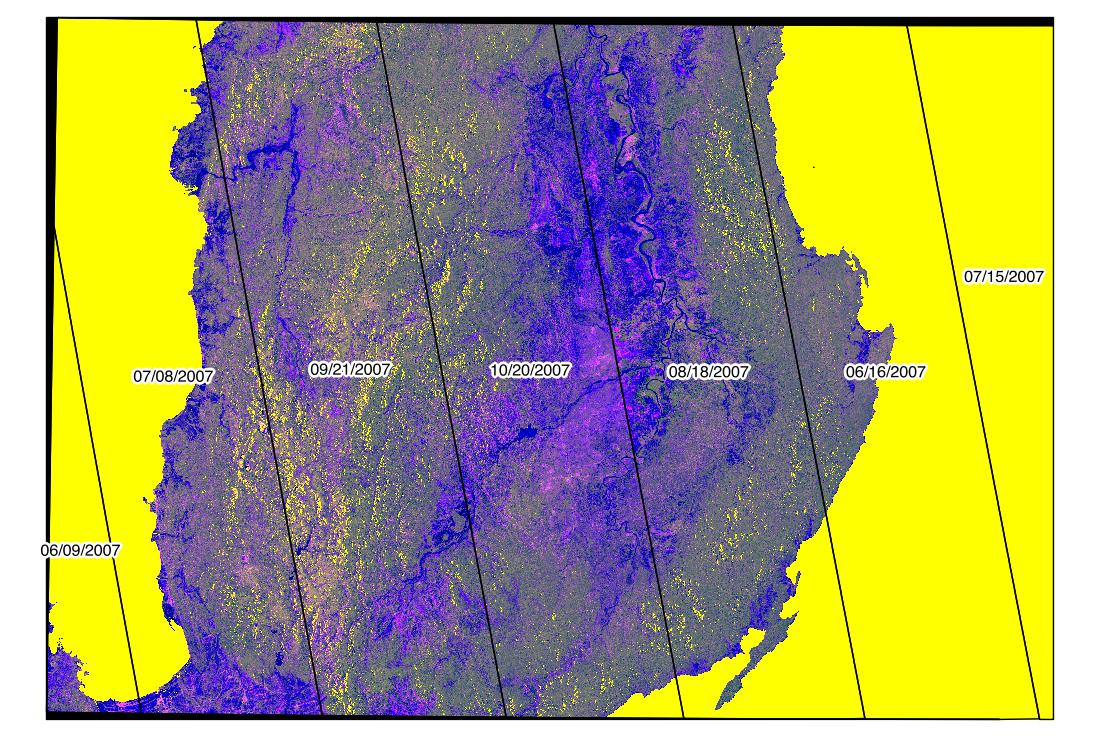
\includegraphics[width=\textwidth]{box_palsar-2007-dates.jpg}
		\caption[Box.1]{}
		\label{box: result-box4.3a}
	\end{subfigure}
	\vspace{5pt}
	\begin{subfigure}[t]{0.75\textwidth}
		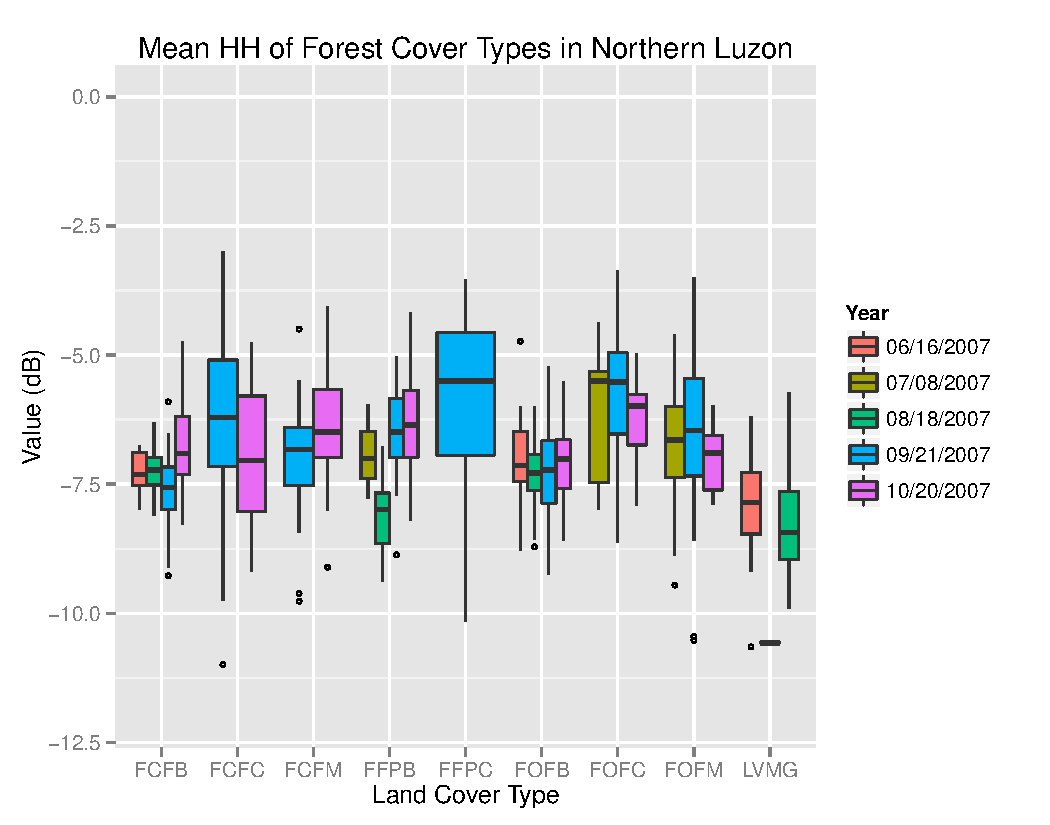
\includegraphics[width=\textwidth]{box_boxplot-2007-mean-hh.pdf}
		\caption[Box.1]{}
		\label{box: result-box4.3b}
	\end{subfigure}\\
	\caption[Box.1. The 2007 PALSAR mosaic image and the dates of acquisition of each strip/path that comprise the whole mosaic, and the distribution of mean HH backscatter for each forest cover type based on the 2007 mosaic image.]{The 2007 PALSAR mosaic image and the dates of acquisition of each strip/path that comprise the whole mosaic (a), and the distribution of mean HH backscatter for each forest cover type (b) based on the 2007 mosaic image.}
	\label{box: result-box4.3}
\end{figure}

\begin{figure}[!ht] \centering
	\captionsetup[subfigure]{width=2.0in} % <-- Use this to control text which is poorly spaced under a subfigure. 
	\begin{subfigure}[t]{0.75\textwidth}
		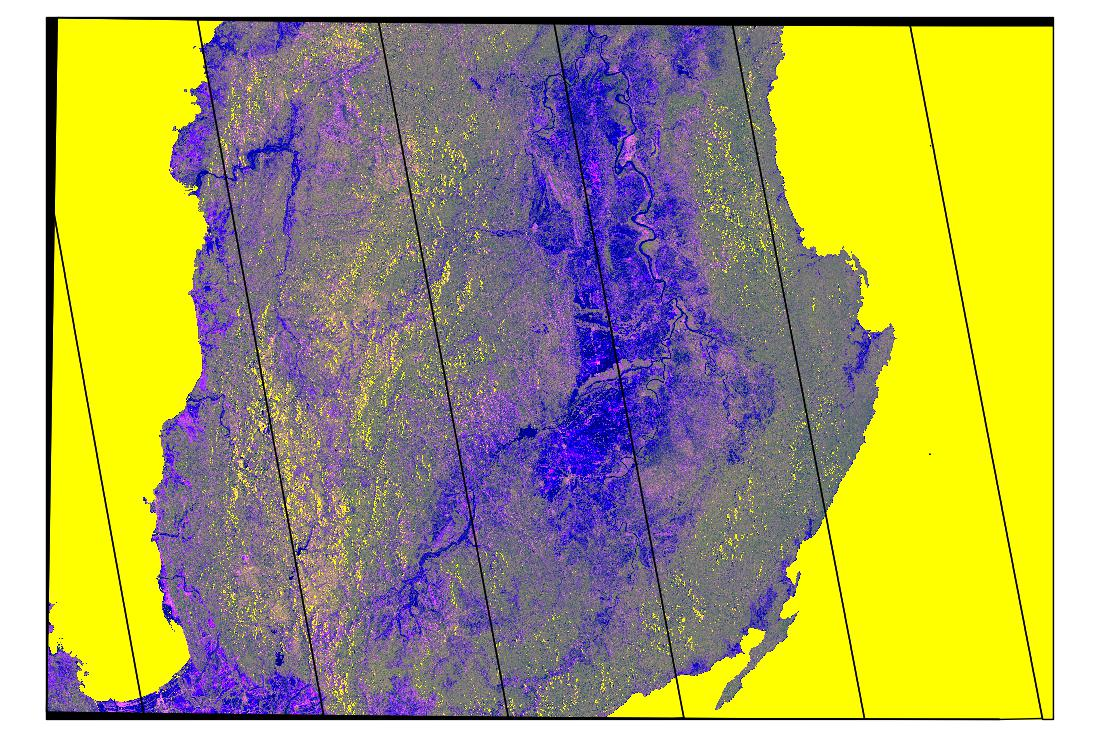
\includegraphics[width=\textwidth]{box_palsar-2010-nodates.jpg}
		\caption[Box.2]{}
		\label{box: result-box4.4a}
	\end{subfigure}
	\vspace{5pt}
	\begin{subfigure}[t]{0.75\textwidth}
		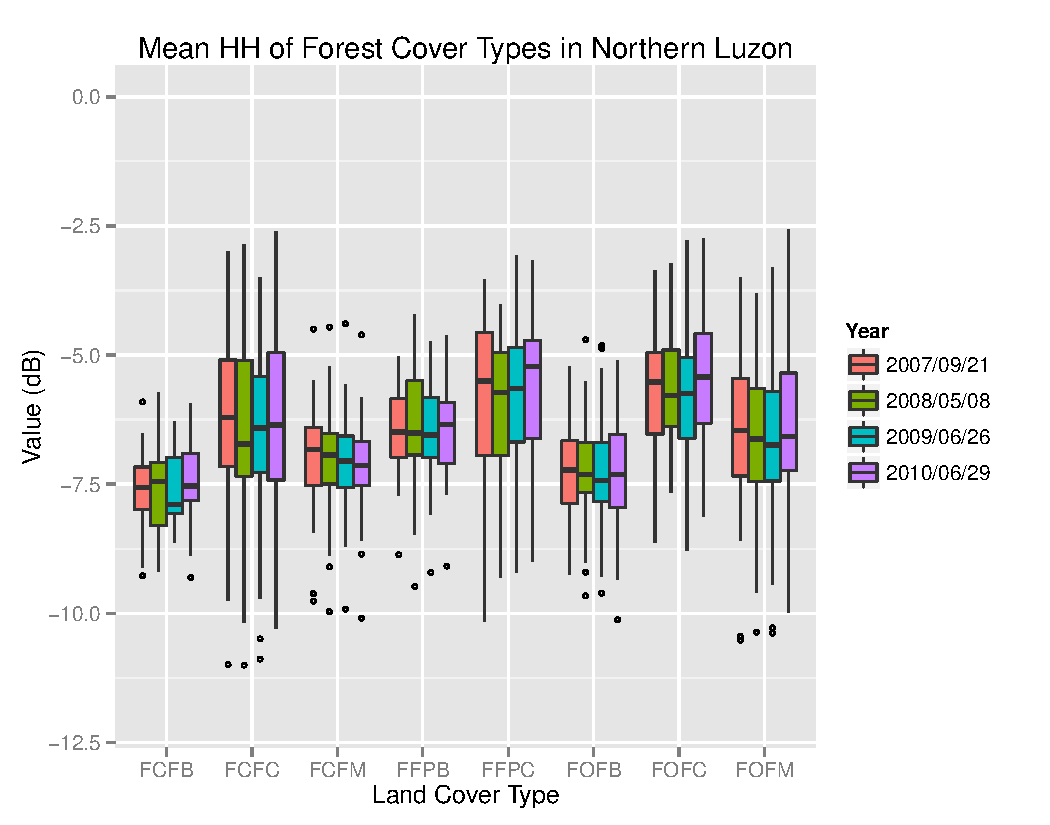
\includegraphics[width=\textwidth]{box_boxplot-strip1-mean-hh.pdf}
		\caption[Box.2]{}
		\label{box: result-box4.4b}
	\end{subfigure}\\
	\caption[Box.2. A PALSAR mosaic image highlighting the strip/path where ROIs of forest cover types were taken across four years, and the distribution of mean HH backscatter for each forest cover type along the same strip at different years.]{A PALSAR mosaic image highlighting the strip/path where ROIs of forest cover types were taken across four years (a), and the distribution of mean HH backscatter for each forest cover type (b) along the same strip at different years.}
	\label{box: result-box4.4}
\end{figure}

\begin{figure}[!ht] \centering
	\captionsetup[subfigure]{width=2.0in} % <-- Use this to control text which is poorly spaced under a subfigure. 
	\begin{subfigure}[t]{0.49\textwidth}
		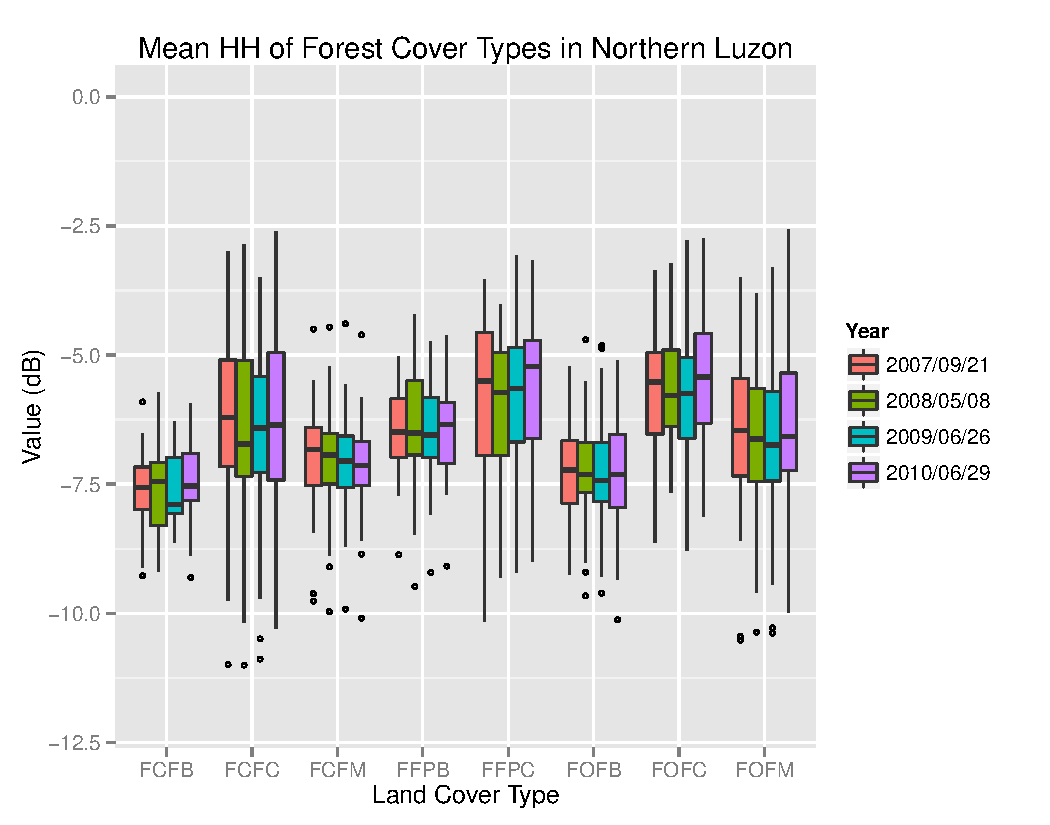
\includegraphics[width=\textwidth]{fig_boxplot-strip1-mean-hh.pdf}
		\caption[Same strip backscatter boxplots.]{Mean HH}
		\label{fig: result-fig4.5a}
	\end{subfigure}
	\begin{subfigure}[t]{0.49\textwidth}
		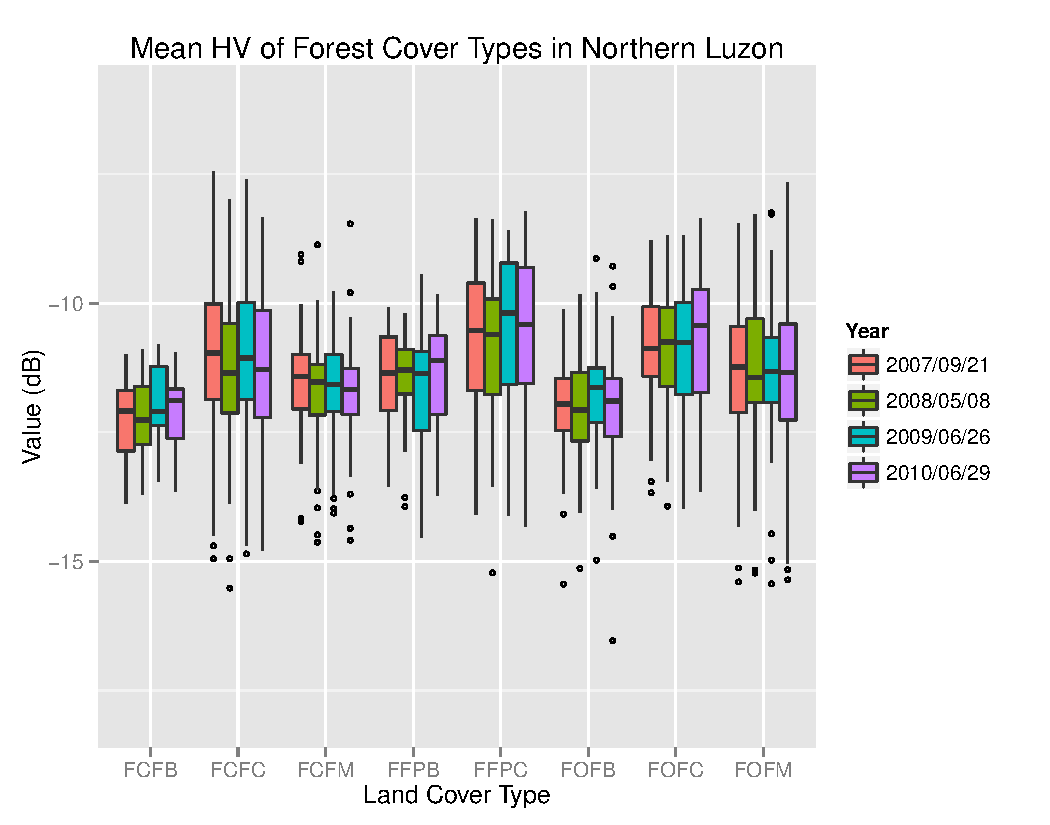
\includegraphics[width=\textwidth]{fig_boxplot-strip1-mean-hv.pdf}
		\caption[Same strip backscatter boxplots.]{Mean HV}
		\label{fig: result-fig4.5b}
	\end{subfigure}\\
	\vspace{10pt}
	\begin{subfigure}[t]{0.49\textwidth}
		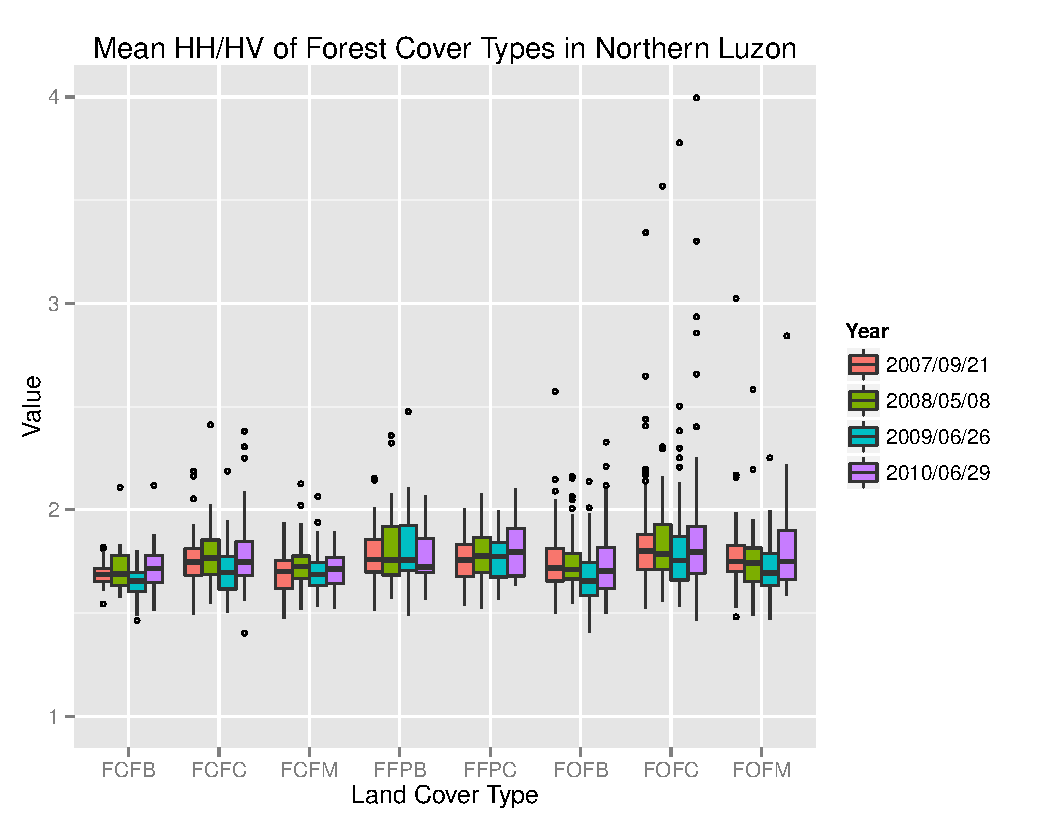
\includegraphics[width=\textwidth]{fig_boxplot-strip1-mean-rat.pdf}
		\caption[Same strip backscatter boxplots.]{Mean HH/HV}
		\label{fig: result-fig4.5c}
	\end{subfigure}
	\begin{subfigure}[t]{0.49\textwidth}
		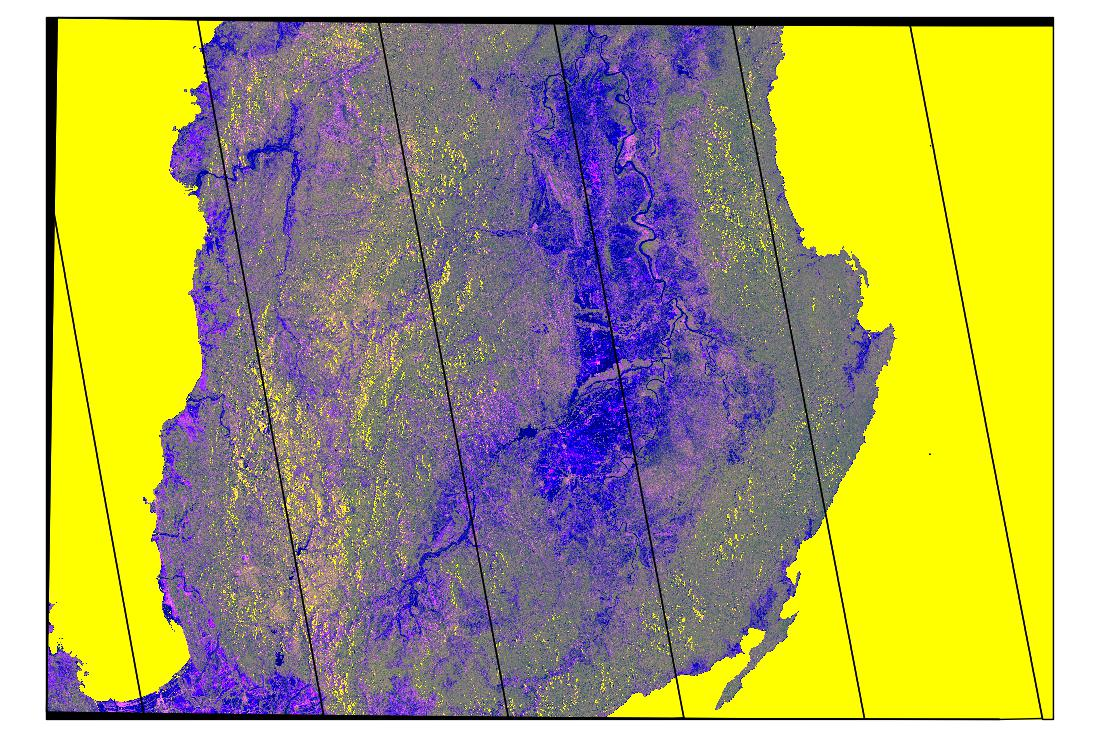
\includegraphics[width=\textwidth]{box_palsar-2010-nodates.jpg}
		\caption[Same strip backscatter boxplots.]{Strip 1}
		\label{fig: result-fig4.5d}
	\end{subfigure}
	\caption[Backscatter values of forest types from PALSAR data acquired along the same strip (Cordillera) at different years.]{Backscatter values of forest types from PALSAR data acquired along the same strip (Cordillera) at different years.}
	\label{fig: result-fig4.5}
\end{figure}

\begin{figure}[!ht] \centering
	\captionsetup[subfigure]{width=2.0in} % <-- Use this to control text which is poorly spaced under a subfigure. 
	\begin{subfigure}[t]{0.49\textwidth}
		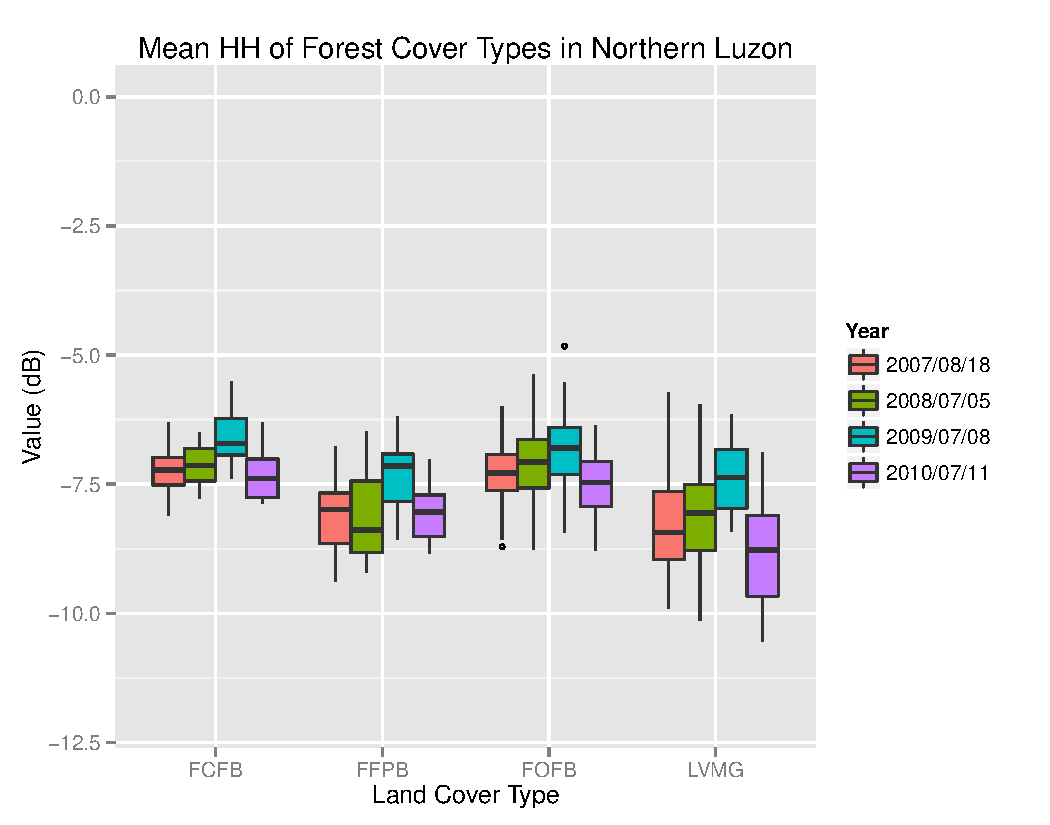
\includegraphics[width=\textwidth]{fig_boxplot-strip2-mean-hh.pdf}
		\caption[Same strip backscatter boxplots.]{Mean HH}
		\label{fig: result-fig4.6a}
	\end{subfigure}
	\begin{subfigure}[t]{0.49\textwidth}
		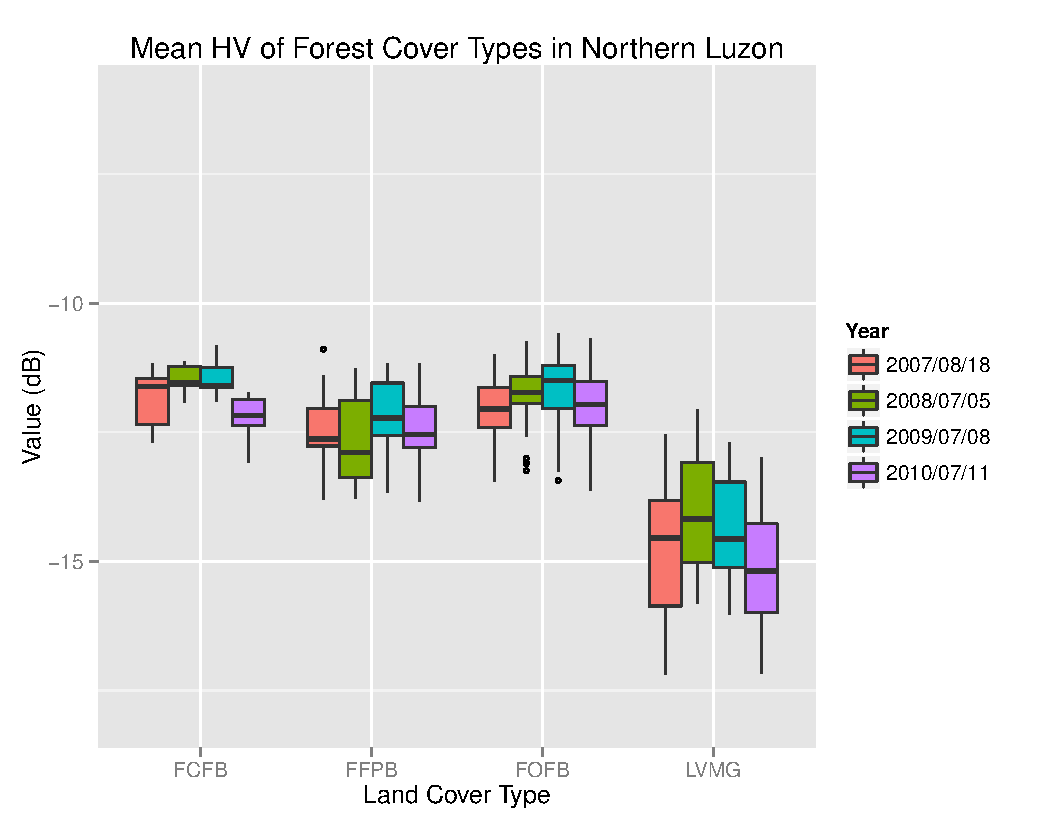
\includegraphics[width=\textwidth]{fig_boxplot-strip2-mean-hv.pdf}
		\caption[Same strip backscatter boxplots.]{Mean HV}
		\label{fig: result-fig4.6b}
	\end{subfigure}\\
	\vspace{10pt}
	\begin{subfigure}[t]{0.49\textwidth}
		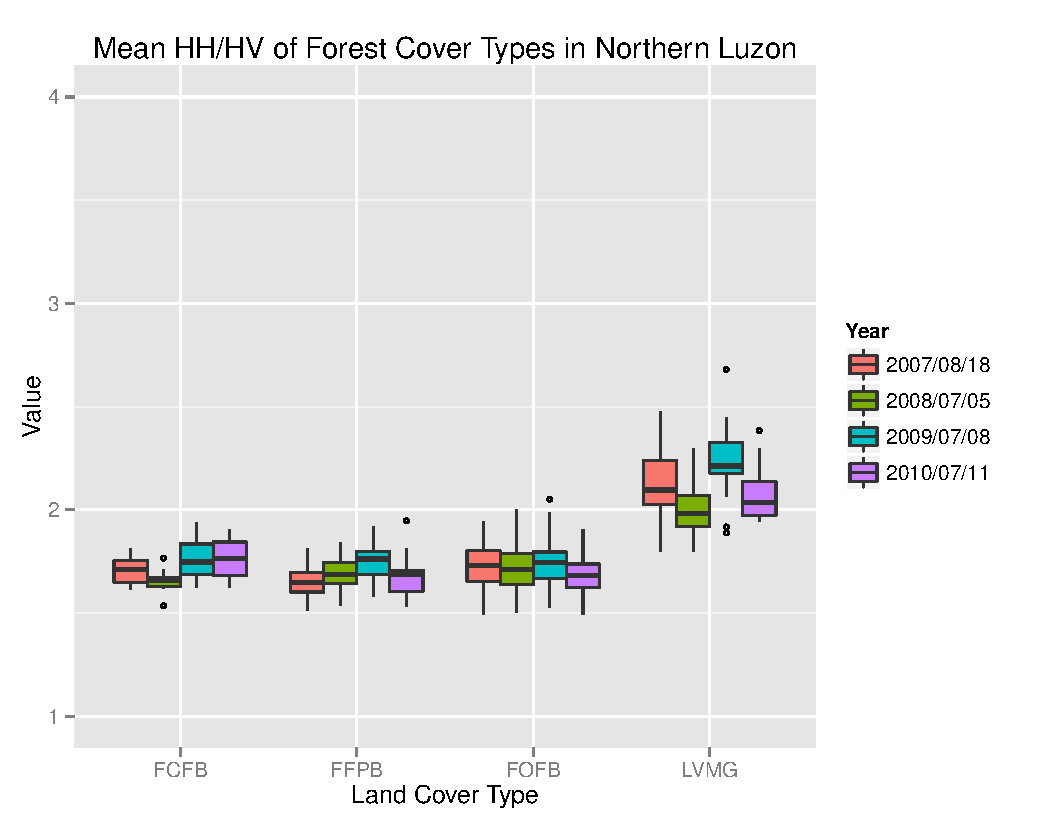
\includegraphics[width=\textwidth]{fig_boxplot-strip2-mean-rat.pdf}
		\caption[Same strip backscatter boxplots.]{Mean HH/HV}
		\label{fig: result-fig4.6c}
	\end{subfigure}
	\begin{subfigure}[t]{0.49\textwidth}
		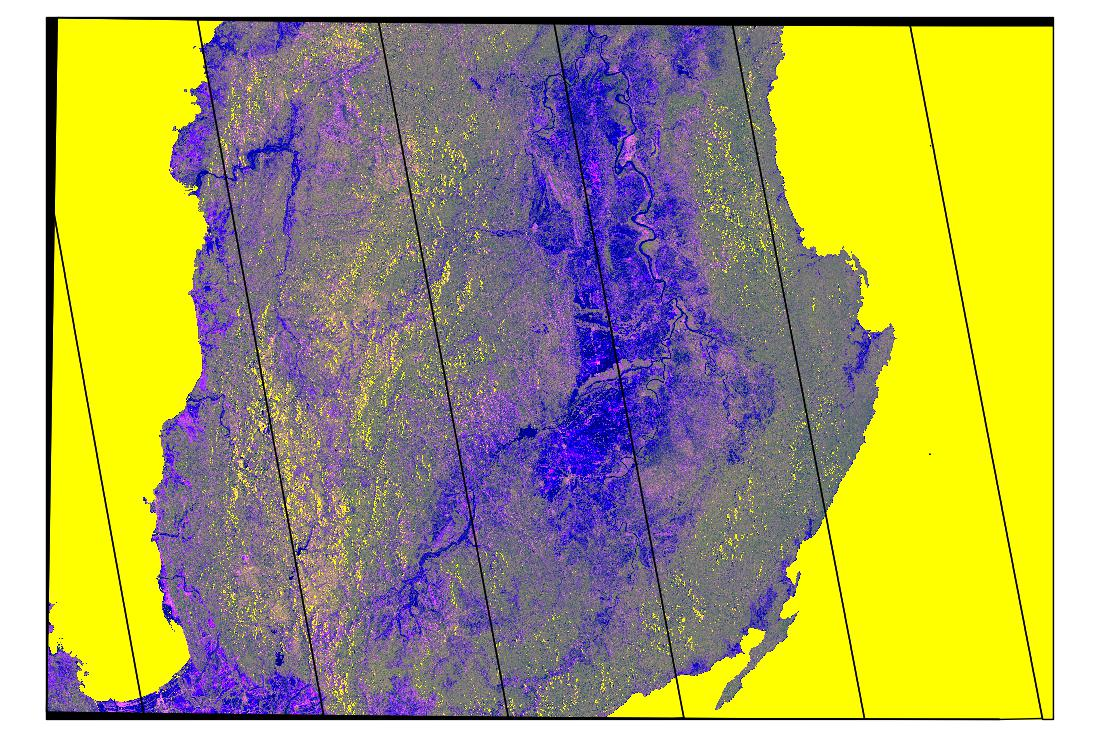
\includegraphics[width=\textwidth]{box_palsar-2010-nodates.jpg}
		\caption[Same strip backscatter boxplots.]{Strip 2}
		\label{fig: result-fig4.6d}
	\end{subfigure}
	\caption[Backscatter values of forest types from PALSAR data acquired along the same strip (Sierra Madre) at different years.]{Backscatter values of forest types from PALSAR data acquired along the same strip (Sierra Madre) at different years.}
	\label{fig: result-fig4.6}
\end{figure}

\section{Consistency of forest classification hierarchy}
\label{sec: result-hierarchy-consistency}

\begin{figure}
	\centering
	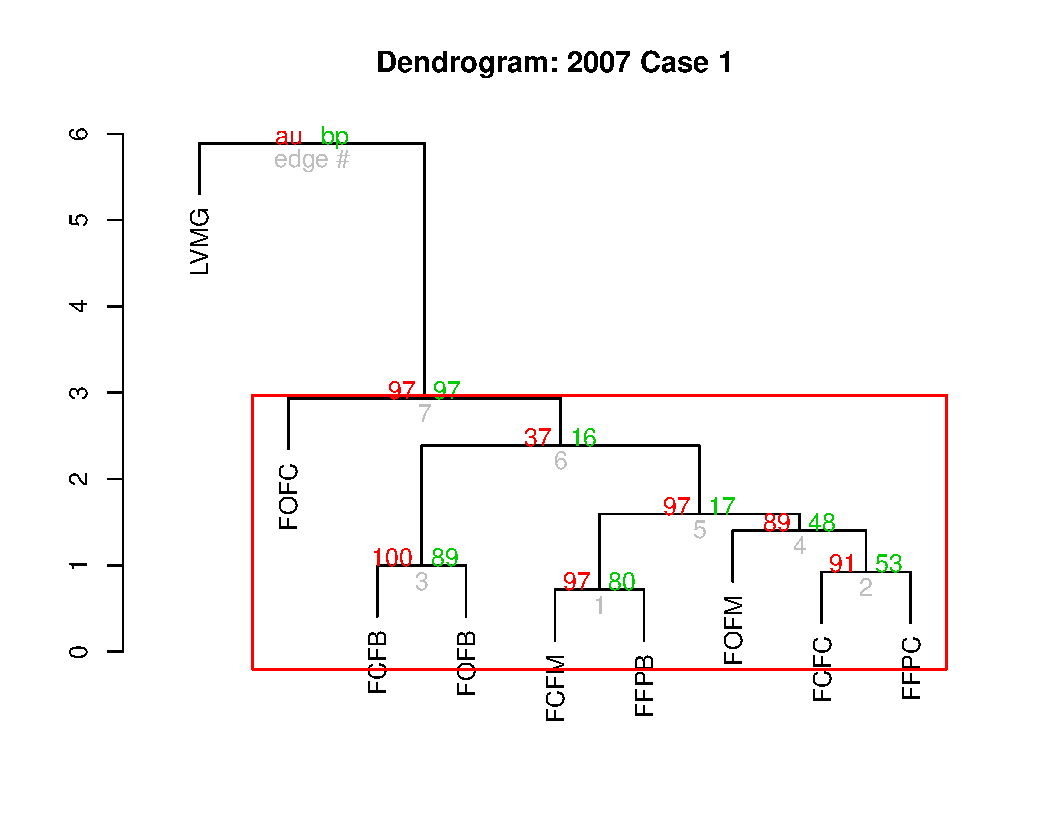
\includegraphics[width=1.0\textwidth]{box_dendrogram-2007-case1.pdf}
	\caption[Box 3. Example dendrogram result from the hierarchical clustering of forest cover types using polarimetric feature attributes (Case 1) from the 2007 PALSAR mosaic image.]{Example dendrogram result from the hierarchical clustering of forest cover types using polarimetric feature attributes (Case 1) from the 2007 PALSAR mosaic image.}
	\label{fig: result-fig4.7}
\end{figure}

A total of 16 dendrograms were produced from the hierarchical cluster analysis consisting of four dendrograms for each case (covering four years in each case). Each case represents a combination of object-level feature attributes (Table \ref{tab: method-table3.3}), particularly: Case 1 using Polarisation feature attributes; Case 2 using Polarisation and Topographic; Case 3 using Polarisation and Texture; and Case 4 using all feature attributes (Polarisation, Topographic, Texture).

As an example, the figure in Fig. \ref{fig: result-fig4.7}, which was taken from Fig. \ref{fig: result-fig4.8}, shows the dendrogram resulting from the hierarchical clustering of forest cover types using polarimetric feature attributes from the 2007 PALSAR mosaic image. The dendrogram shows which forest types are similar or dissimilar from other types. The y-axis indicates the computed distance between clusters using an average linkage algorithm in determining which clusters are similar. Within the tree structure, the edge numbers denoted in grey colour indicate the sequence of the grouping of nodes into similar clusters given that an agglomerative hierarchical clustering technique was used, and the red value indicates the AU p-value, of which values $\geq$ 0.95 represents consistent grouping. The red box indicates which clusters or groups of clusters have $\geq$ 0.95 AU p-values, and hence have consistent groupings.

In this dendrogram, Cluster \#1 showed that closed canopy mixed forest (FCFM) and broadleaved forest plantation (FFPB) were similar with a 97 AU p-value. Next, Cluster \#2 showed closed canopy coniferous forest (FCFC) and coniferous forest plantation (FFPC) were similar with 91 AU p-value. Cluster \#3 showed closed canopy broadleaved forest (FCFB) and open canopy broadleaved forest (FOFB) were similar with 100 AU p-value, suggesting that closed and open canopy broadleaved forests were similar in this case using polarimetric attributes. Cluster \#4 showed Cluster \#2 being grouped together with open canopy mixed forest (FOFM) at 89 AU p-value, and subsequently grouped with Cluster \#1 as Cluster \#5 at 97 AU p-value. All the forest types in Cluster \#5 were subsequently grouped together with Cluster \#3 at only 37 AU p-value. Then, all the forest types in Cluster \#6 were grouped with open canopy coniferous forest (FOFC) as Cluster \#7 with 97 AU p-value. Finally, Cluster \#8 showed mangrove forest (LVMG) grouped with all other forest types in Cluster \#7, suggesting that mangroves had greatest dissimilarity from the rest of the forest types.\\

\begin{spacing}{1.0}
\begin{longtable}[h!]{ p{2.5cm} p{2.6cm} p{2.8cm} p{2.6cm} p{2.5cm} }

    \caption[Baker's Gamma Indices ($\beta$ coefficients) per case for each pair of years.]{Baker's Gamma Indices ($\beta$ coefficients) per case for each pair of years.}
    \label{tab: result-table4.1}\\
    
    	\toprule
    	Years & {} & Baker's Gamma & ($\beta$ Coefficient) & {}\\
    	\cmidrule{2-5}
    	{} & Case 1 & Case 2 & Case 3 & Case 4\\
    	\midrule
    	\endhead
    	
		2007-2008 & 0.8966454 & 0.9896552 & 0.8786650 & 0.8797485\\
		2007-2009 & 0.8527756 & 0.5834679 & 0.8078116 & 0.8393977\\
		2007-2010 & 0.8849630 & 0.9634359 & 0.8301529 & 0.8250326\\
		2008-2009 & 0.8853727 & 0.6208636 & 0.8750541 & 0.8914641\\
		2008-2010 & 0.9899121 & 0.9706925 & 0.8943540 & 0.8950236\\
		2009-2010 & 0.8858105 & 0.6269121 & 0.9539378 & 0.8526550\\
				
		\bottomrule \\
    
\end{longtable}
\end{spacing}

For Case 1, the dendrograms showed the clustering of forest types using only polarimetric feature attributes (Fig. \ref{fig: result-fig4.8}). Except for 2009, AU p-values for the other years were all greater than 0.95 indicating reliable clustering results, specifically for 8 of 9 forest types. Mangrove forest (LVMG) and open coniferous forest (FOFC) appeared as distinct clusters across all years. The $\beta$ coefficients were all high (\textgreater0.85), which indicate relatively similar clusters or dendrogram structure across all four years (Table \ref{tab: result-table4.1}).

For Case 2, the dendrograms showed the clustering of forest types using polarimetric and topographic feature attributes (Fig. \ref{fig: result-fig4.9}). Both 2007 and 2008 exhibited AU p-values above 0.95. For 2009, only two clusters exhibited above 0.95 AU p-values, while 2010 did not at all. Mangrove forest (LVMG) also appeared as distinct clusters across all years. The $\beta$ coefficients were high (\textgreater0.96) for pairwise combinations that do not include 2009, of which values were average (range from 0.58 to 0.63) (Table \ref{tab: result-table4.1}). Interestingly, except 2009, broadleaved forest types (i.e., closed, open, and plantation) and both coniferous and mixed forest types (i.e., closed, open, and plantation) branched into separate clusters, suggesting the distinction of these general forest types.

For Case 3, the dendrograms showed the clustering of forest types using polarimetric and texture feature attributes (Fig. \ref{fig: result-fig4.10}). All years exhibited stable clustering results for 8 of 9 forest types, except 2009 with only 7 of 9 forest types. Mangrove forest (LVMG) and coniferous forest plantations (FFPC) appeared as distinct clusters across all years. The $\beta$  coefficients were all high (\textgreater0.80), which indicate relatively similar clusters or dendrogram structures across all four years (Table \ref{tab: result-table4.1}).

For Case 4, the dendrograms showed the clustering of forest types using all feature attributes, including polarimetric, topographic, and texture (Fig. \ref{fig: result-fig4.11}). The AU p-values consisting of majority of forest types were above 0.95 for 2007, 2008, and 2009. For 2010, only one terminal cluster exhibited above 0.95 AU p-value. Similar to Case 3, mangrove forest (LVMG) and coniferous forest plantations (FFPC) appeared as distinct clusters across all years. The $\beta$ coefficients were all high (\textgreater0.82), which indicate relatively similar clusters or dendrogram structure across all four years (Table \ref{tab: result-table4.1}).\\

\begin{spacing}{1.0}
\begin{longtable}[h!]{ p{1cm} p{1.4cm} p{1.4cm} p{1.4cm} p{1.4cm} p{1.4cm} p{1.4cm} p{1.4cm} p{0.9cm} }

    \caption[Summary of Baker's Gamma Indices ($\beta$ coefficients) for pairwise comparison of dendrograms across all cases.]{Summary of Baker's Gamma Indices ($\beta$ coefficients) for pairwise comparison of dendrograms across all cases.}
    \label{tab: result-table4.2}\\
    
    	\toprule
    	Case & {} 07-08 & 07-09 & 07-10 & 08-09 & 08-10 & 09-10 & Total & Rank\\
    	\midrule
    	\endhead
    	
		1 & 0.89664 & 0.85277 & 0.88496 & 0.88537 & 0.98991 & 0.88581 & 5.39547 & 1\\
		2 & 0.98965 & 0.58346 & 0.96343 & 0.62086 & 0.97069 & 0.62691 & 4.75502 & 4\\
		3 & 0.87866 & 0.80781 & 0.83015 & 0.87505 & 0.89435 & 0.95393 & 5.23997 & 2\\
		4 & 0.87974 & 0.83939 & 0.82503 & 0.89146 & 0.89502 & 0.85265 & 5.18332 & 3\\
		\cmidrule{1-9}
		Total & 3.64471 & 3.08345 & 3.50358 & 3.27275 & 3.74998 & 3.31931 & 3.42896 & {}\\
				
		\bottomrule \\
    
\end{longtable}
\end{spacing}

The Baker's Gamma Indices for pairwise comparison of dendrograms were tabulated across all cases to assess the effect of topographic and texture feature attributes, in addition to polarisation, on the consistency of the hierarchies between dendrograms (Table \ref{tab: result-table4.2}). Pairwise dendrogram comparisons involving the 2009 ALOS/PALSAR image showed lower consistencies as shown by vertical sum of coefficients for each pairwise comparison.

High Baker's Gamma Index coefficients (i.e., values close to 1) resulting from pairwise comparisons of dendrograms between acquisition years indicated that the hierarchical clustering of forest types were similar and consistent across years, and reinforced the temporal consistency of the ALOS/PALSAR mosaic data acquired in different years. Ranking showed that polarimetric variables (Case 1) had the highest consistencies between pairwise dendrogram comparisons. This suggests that polarimetric data by itself is temporally consistent across different acquisition years, and the forest classification hierarchy is also similarly consistent across different acquisition years. The inclusion of other feature attributes slightly lowers the consistency in both aspects. Nevertheless, nominal values of Baker’s Gamma Index coefficients were still high, suggesting that the inclusion of topographic or texture variables or both only marginally decreases the temporal consistency of ALOS/PALSAR mosaics and hierarchical consistency of the forest type classification.

\begin{figure}[!ht] \centering
	\captionsetup[subfigure]{width=2.0in} % <-- Use this to control text which is poorly spaced under a subfigure. 
	\begin{subfigure}[t]{0.49\textwidth}
		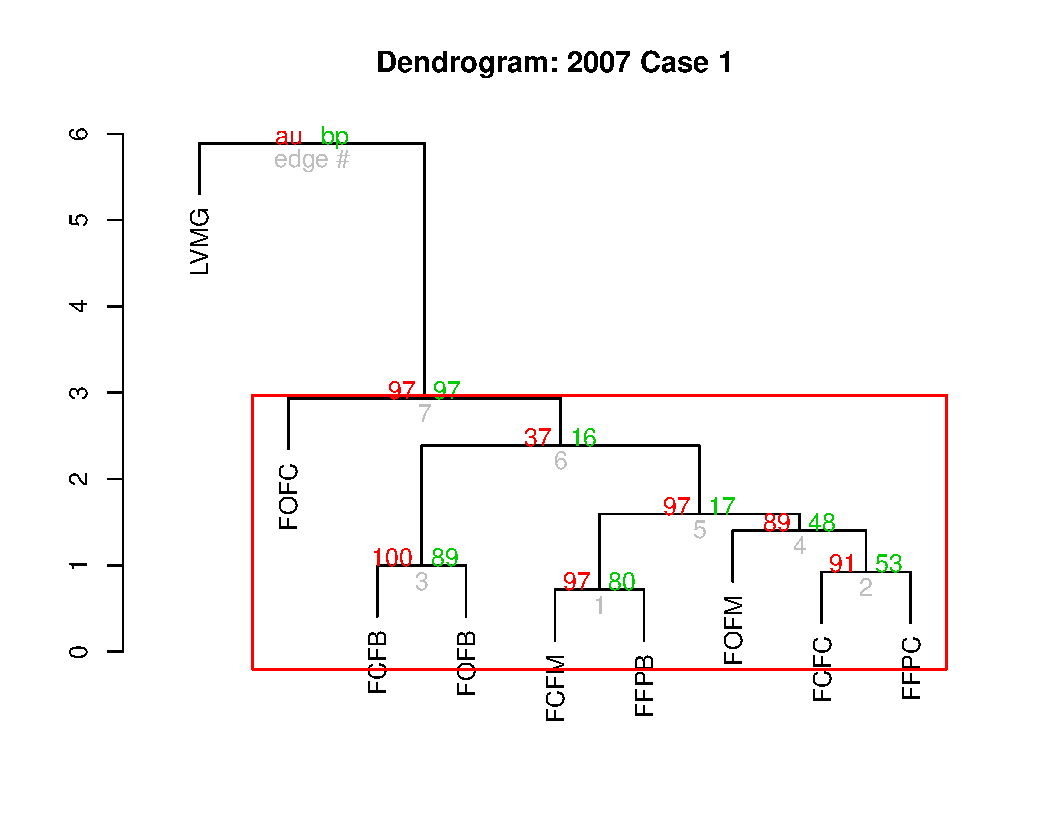
\includegraphics[width=\textwidth]{fig_dendrogram-2007-case1.pdf}
		\caption[Case 1 cluster dendrograms.]{2007 Case 1}
		\label{fig: result-fig4.8a}
	\end{subfigure}
	\begin{subfigure}[t]{0.49\textwidth}
		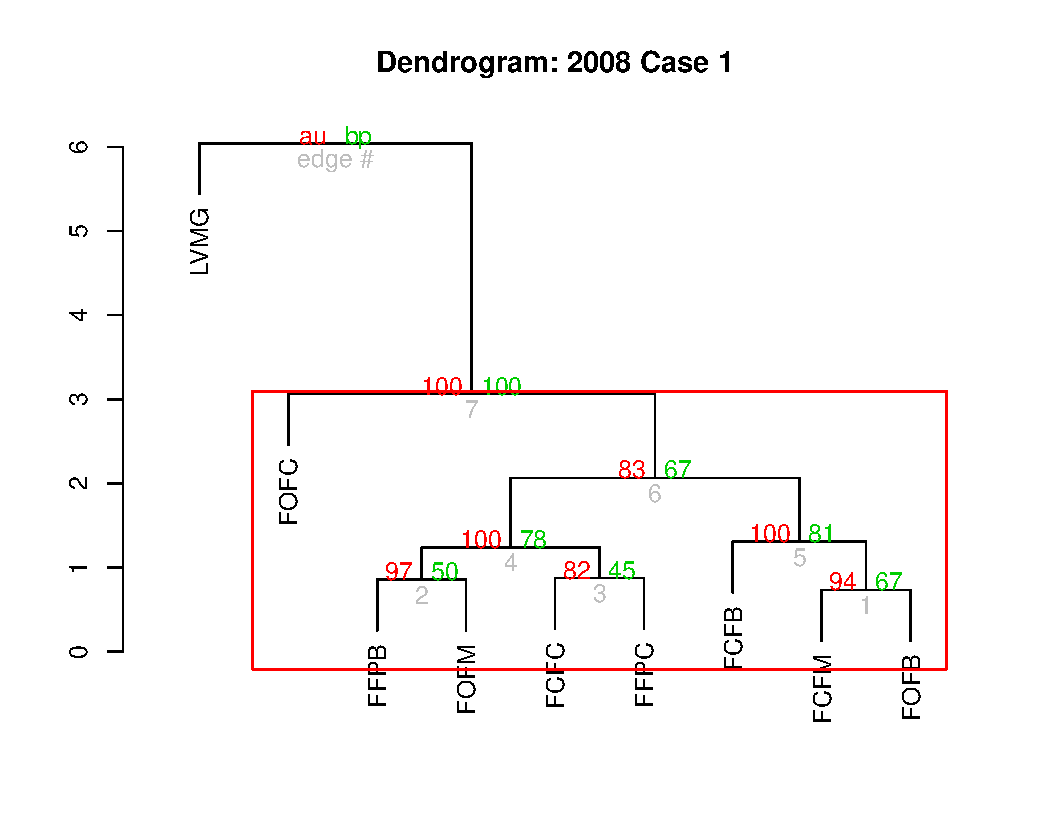
\includegraphics[width=\textwidth]{fig_dendrogram-2008-case1.pdf}
		\caption[Case 1 cluster dendrograms.]{2008 Case 1}
		\label{fig: result-fig4.8b}
	\end{subfigure}\\
	\vspace{15pt}
	\begin{subfigure}[t]{0.49\textwidth}
		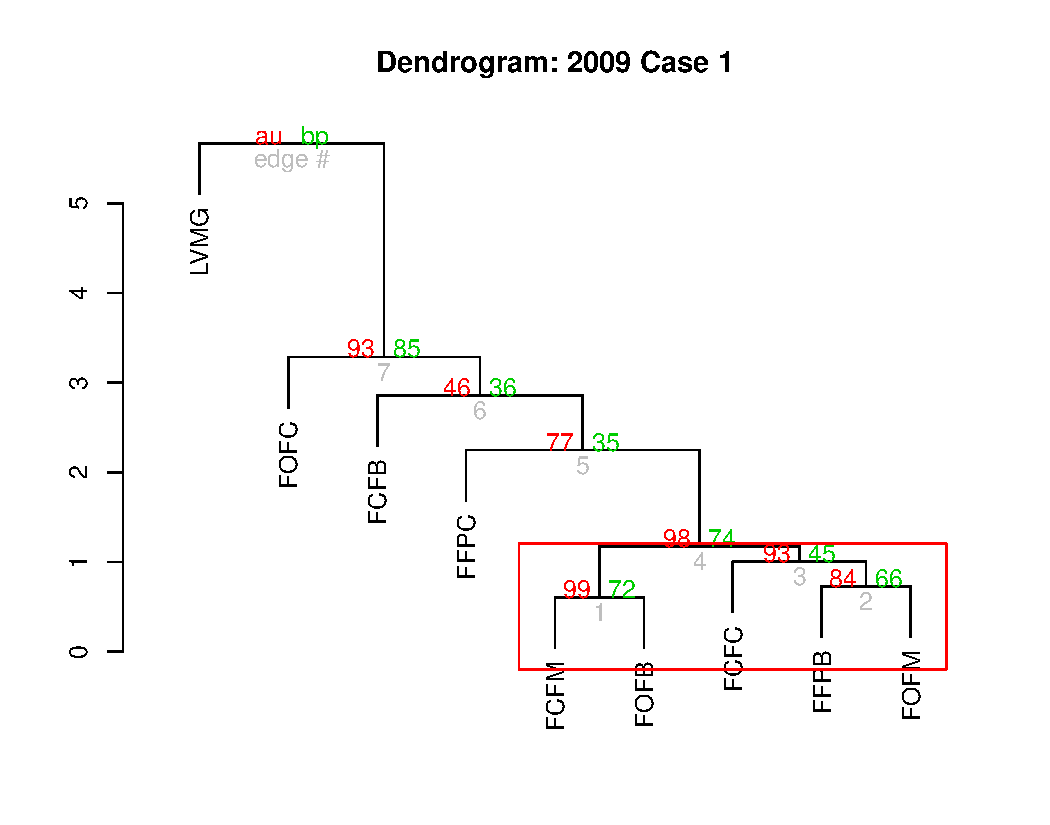
\includegraphics[width=\textwidth]{fig_dendrogram-2009-case1.pdf}
		\caption[Case 1 cluster dendrograms.]{2009 Case 1}
		\label{fig: result-fig4.8c}
	\end{subfigure}
	\begin{subfigure}[t]{0.49\textwidth}
		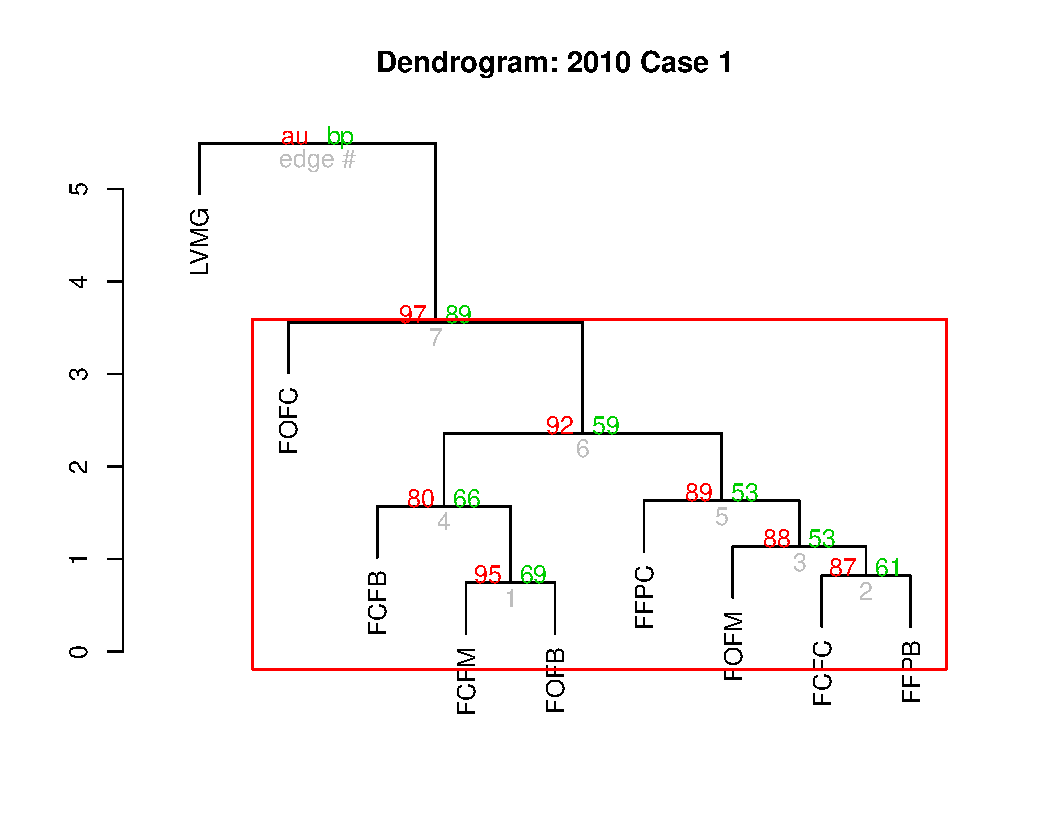
\includegraphics[width=\textwidth]{fig_dendrogram-2010-case1.pdf}
		\caption[Case 1 cluster dendrograms.]{2010 Case 1}
		\label{fig: result-fig4.8d}
	\end{subfigure}
	\vspace{5pt}
	\caption[Dendrograms from cluster analysis using Case 1.]{Dendrograms from cluster analysis using Case 1. Red boxes AU p-value $\geq$ 0.95.}
	\label{fig: result-fig4.8}
\end{figure}

\begin{figure}[!ht] \centering
	\captionsetup[subfigure]{width=2.0in} % <-- Use this to control text which is poorly spaced under a subfigure. 
	\begin{subfigure}[t]{0.49\textwidth}
		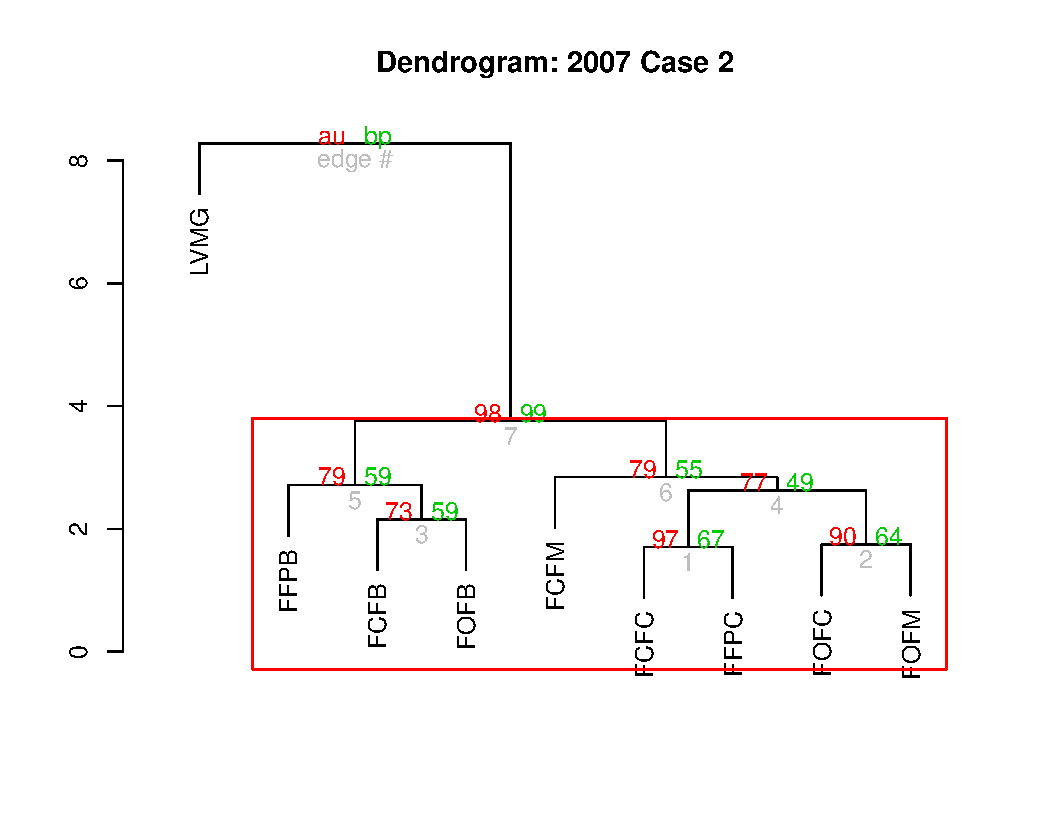
\includegraphics[width=\textwidth]{fig_dendrogram-2007-case2.pdf}
		\caption[Case 2 cluster dendrograms.]{2007 Case 2}
		\label{fig: result-fig4.9a}
	\end{subfigure}
	\begin{subfigure}[t]{0.49\textwidth}
		\includegraphics[width=\textwidth]{fig_dendrogram-2008-case2.pdf}
		\caption[Case 2 cluster dendrograms.]{2008 Case 2}
		\label{fig: result-fig4.9b}
	\end{subfigure}\\
	\vspace{15pt}
	\begin{subfigure}[t]{0.49\textwidth}
		\includegraphics[width=\textwidth]{fig_dendrogram-2009-case2.pdf}
		\caption[Case 2 cluster dendrograms.]{2009 Case 2}
		\label{fig: result-fig4.9c}
	\end{subfigure}
	\begin{subfigure}[t]{0.49\textwidth}
		\includegraphics[width=\textwidth]{fig_dendrogram-2010-case2.pdf}
		\caption[Case 2 cluster dendrograms.]{2010 Case 2}
		\label{fig: result-fig4.9d}
	\end{subfigure}
	\vspace{5pt}
	\caption[Dendrograms from cluster analysis using Case 2.]{Dendrograms from cluster analysis using Case 2. Red boxes AU p-value $\geq$ 0.95.}
	\label{fig: result-fig4.9}
\end{figure}

\begin{figure}[!ht] \centering
	\captionsetup[subfigure]{width=2.0in} % <-- Use this to control text which is poorly spaced under a subfigure. 
	\begin{subfigure}[t]{0.49\textwidth}
		\includegraphics[width=\textwidth]{fig_dendrogram-2007-case3.pdf}
		\caption[Case 3 cluster dendrograms.]{2007 Case 3}
		\label{fig: result-fig4.10a}
	\end{subfigure}
	\begin{subfigure}[t]{0.49\textwidth}
		\includegraphics[width=\textwidth]{fig_dendrogram-2008-case3.pdf}
		\caption[Case 3 cluster dendrograms.]{2008 Case 3}
		\label{fig: result-fig4.10b}
	\end{subfigure}\\
	\vspace{15pt}
	\begin{subfigure}[t]{0.49\textwidth}
		\includegraphics[width=\textwidth]{fig_dendrogram-2009-case3.pdf}
		\caption[Case 3 cluster dendrograms.]{2009 Case 3}
		\label{fig: result-fig4.10c}
	\end{subfigure}
	\begin{subfigure}[t]{0.49\textwidth}
		\includegraphics[width=\textwidth]{fig_dendrogram-2010-case3.pdf}
		\caption[Case 3 cluster dendrograms.]{2010 Case 3}
		\label{fig: result-fig4.10d}
	\end{subfigure}
	\vspace{5pt}
	\caption[Dendrograms from cluster analysis using Case 3.]{Dendrograms from cluster analysis using Case 3. Red boxes AU p-value $\geq$ 0.95.}
	\label{fig: result-fig4.10}
\end{figure}

\begin{figure}[!ht] \centering
	\captionsetup[subfigure]{width=2.0in} % <-- Use this to control text which is poorly spaced under a subfigure. 
	\begin{subfigure}[t]{0.49\textwidth}
		\includegraphics[width=\textwidth]{fig_dendrogram-2007-case4.pdf}
		\caption[Case 4 cluster dendrograms.]{2007 Case 4}
		\label{fig: result-fig4.11a}
	\end{subfigure}
	\begin{subfigure}[t]{0.49\textwidth}
		\includegraphics[width=\textwidth]{fig_dendrogram-2008-case4.pdf}
		\caption[Case 4 cluster dendrograms.]{2008 Case 4}
		\label{fig: result-fig4.11b}
	\end{subfigure}\\
	\vspace{15pt}
	\begin{subfigure}[t]{0.49\textwidth}
		\includegraphics[width=\textwidth]{fig_dendrogram-2009-case4.pdf}
		\caption[Case 4 cluster dendrograms.]{2009 Case 4}
		\label{fig: result-fig4.11c}
	\end{subfigure}
	\begin{subfigure}[t]{0.49\textwidth}
		\includegraphics[width=\textwidth]{fig_dendrogram-2010-case4.pdf}
		\caption[Case 4 cluster dendrograms.]{2010 Case 4}
		\label{fig: result-fig4.11d}
	\end{subfigure}
	\vspace{5pt}
	\caption[Dendrograms from cluster analysis using Case 4.]{Dendrograms from cluster analysis using Case 4. Red boxes AU p-value $\geq$ 0.95.}
	\label{fig: result-fig4.11}
\end{figure}

\section{Accuracy of multi-level hierarchical classification approach}
\label{sec: result-accuracy-hierarchical}

Classification trees were generated for all cases or combinations of feature attributes for all years (Appendix \ref{app: appendix-trees-graphs}). For each case, 11 trees were generated from running the decision tree classification in each year, totalling 44 classification trees for one case across four years. Each tree corresponds to one of 11 classification levels based on the multi- level classification hierarchy, of which is defined by a chosen cluster dendrogram (discussed later).

An example of the generated classification trees is shown in Fig. \ref{fig: result-fig4.12} (from Appendix \ref{app: appendix-trees-graphs}), which shows four classification trees corresponding to the first four classification levels at Case 1 of the 2007 PALSAR mosaic image. Classification Level 1 splits into either Land or Water classes. Then at Level 2, with the Water class set aside, the Land class was split into either Vegetation or Non-Vegetation classes. At Level 3, the Vegetation class was split into either Forest or Non-Forest classes while the Non- Vegetation class was set aside. For Level 4, with the Non-Forest class set aside, the Forest class was split into either Mangrove forest or the other forest types group (here denoted as Forest Group 7). To interpret the classification tree, the data is split starting at top level of the tree, in this case looking at Level 1 classification tree as an example. The tree is split into two branches using Mean HH as the predictor variable, of which values less than -10.6321 in HH backscatter are assigned into the left branch, and those greater than this value are assigned into the right branch. Considering the left branch first, it is then subsequently split again into two branches again using Mean HV as the predictor variable. In this case, however, regardless whether the values are less than or greater than -20.2073 in HV backscatter, these are assigned into the Water class, which are the terminal nodes. Next, considering the right branch from the topmost node, it is split using Mean HV as the predictor variable, of which values less than -13.8405 in HV backscatter are assigned into the left branch, and those greater than this value are assigned into the right branch. Again, treating the left branch first, it is split using SD of HV layer with values less than 1.78303 assigned into the Land class and those greater than this value are assigned into the Water class, which are also both terminal nodes. Lastly, treating the right branch, it is split using Mean HV as the predictor variable. Again in this case, regardless of whether the values are less than or greater than -12.7619 in HV backscatter, these are assigned into the Land class. Once the data in Level 1 are all assigned into either the Land or Water classes, the Water class are set aside, and the data assigned to the Land class are then classified using the Level 2 classification tree, splitting into either Vegetation or Non-Vegetation classes. The classification process continues until all the data are assigned to classes ending at the Level 11 classification tree.

\begin{figure}[!ht] \centering
	\captionsetup[subfigure]{width=2.0in} % <-- Use this to control text which is poorly spaced under a subfigure. 
	\begin{subfigure}[t]{0.49\textwidth}
		\includegraphics[width=\textwidth]{box_2007-pruned-dendrogram-lc1.pdf}
		\caption[Box.4]{Level 1}
		\label{fig: result-fig4.12a}
	\end{subfigure}
	\begin{subfigure}[t]{0.49\textwidth}
		\includegraphics[width=\textwidth]{box_2007-pruned-dendrogram-lc2.pdf}
		\caption[Box.4]{Level 2}
		\label{fig: result-fig4.12b}
	\end{subfigure}\\
	\vspace{15pt}
	\begin{subfigure}[t]{0.49\textwidth}
		\includegraphics[width=\textwidth]{box_2007-pruned-dendrogram-lc3.pdf}
		\caption[Box.4]{Level 3}
		\label{fig: result-fig4.12c}
	\end{subfigure}
	\begin{subfigure}[t]{0.49\textwidth}
		\includegraphics[width=\textwidth]{box_2007-pruned-dendrogram-lc4.pdf}
		\caption[Box.4]{Level 4}
		\label{fig: result-fig4.12d}
	\end{subfigure}
	\vspace{5pt}
	\caption[Box 4. Example classification trees corresponding to the first four classification levels at Case 1 of the 2007 PALSAR mosaic image.]{Example classification trees corresponding to the first four classification levels at Case 1 of the 2007 PALSAR mosaic image. Shown are Level 1 (land-water), Level 2 (vegetation - non-vegetation), Level 3 (forest - non-forest), and Level 4 (mangrove - non-mangrove).}
	\label{fig: result-fig4.12}
\end{figure}

The error rates obtained at each classification level per case per year were tabulated (Appendix \ref{app: appendix-error-rates}). Two sets of plots were generated: the first set of plots presented per case compared the error rates obtained for each year across classification levels (Fig. \ref{fig: result-fig4.13}); the second set of plots presented per year compared the error rates for each case across classification levels (Fig. \ref{fig: result-fig4.14}).

In Fig. \ref{fig: result-fig4.13}, the misclassification error rates across all years for all cases followed a consistent trend from classification levels 1 to 5, and turned erratic with no clear trend from classification level 6 onwards. Error rates at the first two classification levels were consistently very low across all years, indicating the suitability of PALSAR mosaics for discriminating between Land and Water (Level 1) and Vegetation and Non-Vegetation (Level 2), and this consistency was observed for multi-year PALSAR mosaics.

At Level 1, error rates decreased from Case 1 to Case 4, of which Case 4 had the lowest error rates, suggesting that the inclusion of topographic, texture, or both in addition to polarimetric variables improved classification accuracy. At Level 2, Case 2 and Case 4 showed lower error rates compared to the other two cases, suggesting that inclusion of topographic variables (Case 2) or all variables (Case 4) resulted in better separation of Vegetation and Non-Vegetation classes. Between Case 2 and Case 4, however, no significant differences in error rates were observed, suggesting that the addition of topographic variables (Case 2) or topographic and texture (Case 4) to polarimetric variables can produce the same result. At Level 3, Case 2 and Case 4 also showed lower error rates compared to the other two cases, suggesting the inclusion again of topographic variables or all variables can provide better discrimination of Forest and Non-Forest classes. At Level 4, mangrove forest (LVMG) was consistently separated from the other forest types across all cases and across all years. Notably, error rates at Level 4 resulted into zero for cases that involved topographic attributes, particularly at Case 2 and Case 4, which was primarily due to elevation—and nothing else—as the most parsimonious variable that discriminated mangroves from other forest types (Appendix \ref{app: appendix-error-rates}). This indicates that the decision tree classifier selected elevation as a determining variable for classifying mangrove forests, which is true since mangroves are situated on low elevations. However, elevation as the sole variable determining the classification of mangroves is not feasible as not all areas on low elevation are mangroves. Case 1 and Case 3 both showed low error rates in discriminating between mangrove forest and other forest types. Between the two cases, Case 3 showed slightly lower error rates compared to Case 1 suggesting that adding texture variables to polarimetric variables can marginally improve the classification accuracy. At Level 5, open canopy coniferous forest (FOFC) was consistently discriminated from other forest types in Case 1 across all years. In Case 2, closed canopy broadleaved forest (FCFB) was consistently discriminated from other forest types across all years. For Case 3 and Case 4, coniferous forest plantation (FFPC) was consistently discriminated from other forest types across all years. This particular discrimination of one forest type from the others may suggest the influence of specific predictor variables (or combinations thereof) for discriminating these forest types at this classification level. Finally, for Level 6 onwards, no apparent trend was observed except the erratic behaviour of the graphs of error rates, suggesting the varied influence of predictor variables at specific cases in the discrimination of forest types.

In Fig. \ref{fig: result-fig4.14}, the misclassification error rates were presented this time per year to compare each case across classification levels. Similar to Fig. \ref{fig: result-fig4.13}, error rates across all cases for all years followed a consistent trend from classification levels 1 to 5, and turned erratic with no clear trend from classification level 6 onwards. The error rates at the first two classification levels, specifically Level 1 (Land and Water) and Level 2 (Vegetation and Non-Vegetation) were consistently very low across cases for all years. The error rates spiked at Level 3 (Forest and Non-Forest) for all cases, of which Case 2 and Case 4 exhibited the lower error rates compared to the other cases (Appendix \ref{app: appendix-error-rates}), and subsequently Case 4 had the lowest error rates compared to Case 2. At Level 4, error rates were low for Case 1 and Case 3, and resulted to 0 for Case 2 and 4. At Level 5, Case 1 and 2 showed higher error rates compared to the other two cases across all years.\\

\begin{figure}[!ht] \centering
	\captionsetup[subfigure]{width=2.0in} % <-- Use this to control text which is poorly spaced under a subfigure. 
	\begin{subfigure}[t]{0.49\textwidth}
		\includegraphics[width=\textwidth]{fig_graph-pruned-case1.pdf}
		\caption[Error rates across levels per case.]{Case 1}
		\label{fig: result-fig4.13a}
	\end{subfigure}
	\begin{subfigure}[t]{0.49\textwidth}
		\includegraphics[width=\textwidth]{fig_graph-pruned-case2.pdf}
		\caption[Error rates across levels per case.]{Case 2}
		\label{fig: result-fig4.13b}
	\end{subfigure}\\
	\vspace{15pt}
	\begin{subfigure}[t]{0.49\textwidth}
		\includegraphics[width=\textwidth]{fig_graph-pruned-case3.pdf}
		\caption[Error rates across levels per case.]{Case 3}
		\label{fig: result-fig4.13c}
	\end{subfigure}
	\begin{subfigure}[t]{0.49\textwidth}
		\includegraphics[width=\textwidth]{fig_graph-pruned-case4.pdf}
		\caption[Error rates across levels per case.]{Case 4}
		\label{fig: result-fig4.13d}
	\end{subfigure}
	\vspace{5pt}
	\caption[Plots comparing error rates obtained for each year across classification levels per case.]{Plots comparing error rates obtained for each year across classification levels per case.}
	\label{fig: result-fig4.13}
\end{figure}

\begin{figure}[!ht] \centering
	\captionsetup[subfigure]{width=2.0in} % <-- Use this to control text which is poorly spaced under a subfigure. 
	\begin{subfigure}[t]{0.49\textwidth}
		\includegraphics[width=\textwidth]{fig_graph-pruned-2007.pdf}
		\caption[Error rates across levels per year.]{2007}
		\label{fig: result-fig4.14a}
	\end{subfigure}
	\begin{subfigure}[t]{0.49\textwidth}
		\includegraphics[width=\textwidth]{fig_graph-pruned-2008.pdf}
		\caption[Error rates across levels per year.]{2008}
		\label{fig: result-fig4.14b}
	\end{subfigure}\\
	\vspace{15pt}
	\begin{subfigure}[t]{0.49\textwidth}
		\includegraphics[width=\textwidth]{fig_graph-pruned-2009.pdf}
		\caption[Error rates across levels per year.]{2009}
		\label{fig: result-fig4.14c}
	\end{subfigure}
	\begin{subfigure}[t]{0.49\textwidth}
		\includegraphics[width=\textwidth]{fig_graph-pruned-2010.pdf}
		\caption[Error rates across levels per year.]{2010}
		\label{fig: result-fig4.14d}
	\end{subfigure}
	\vspace{5pt}
	\caption[Plots comparing error rates obtained for each case across classification levels per year.]{Plots comparing error rates obtained for each case across classification levels per year.}
	\label{fig: result-fig4.14}
\end{figure}

\begin{spacing}{1.0}
\begin{longtable}[h!]{ p{2.6cm} p{2.6cm} p{2.6cm} p{2.6cm} p{2.6cm} }

    \caption[Summary of total classification error rates per case per year.]{Summary of total classification error rates per case per year.}
    \label{tab: result-table4.3}\\
    
    	\toprule
    	Case & 2007 & 2008 & 2009 & 2010\\
    	\midrule
    	\endhead
    	
		1 & 163.745 & 158.784 & 155.709 & 160.277\\
		2 & 101.349 & 103.588 &  91.795 & 102.603\\
		3 &  95.333 & 101.463 &  98.812 &  96.342\\
		4 &  74.556 &  78.679 &  69.118 &  70.525\\
		
		\bottomrule \\
    
\end{longtable}
\end{spacing}

A subsequent summary of the total classification error rates per case per year was computed (Table \ref{tab: result-table4.3}). The table showed that the inclusion of topographic and texture attributes (Case 2 and Case 3, respectively) tend to reduce the misclassification error rates compared to using solely polarimetric attributes (Case 1). The addition of topographic to polarimetric attributes (Case 2) also showed higher error rates compared to a polarimetric and texture combination (Case 3). The inclusion of all feature attributes (Case 4), including polarimetric, topographic, and texture, produced the lowest misclassification error rates across years; and consequently, it formed the bases of the classification hierarchies that were constructed through rulesets to produce the annual land cover maps (Fig. \ref{fig: result-fig4.15}).

The mean error rates of land cover classes for each case and each year were tabulated (Table \ref{tab: result-table4.4}), which indicates that the mean error rates were still the lowest for Case 4 compared to other cases across all years. The inclusion of either topographic or texture attributes to polarimetric data tended to lower the classification error rates, of which error rates with texture included was lower compared to error rates with topographic attributes included. This emphasises that the inclusion of both topographic and texture feature attributes improve the classification accuracy of forest cover types.\\

\begin{spacing}{1.0}
\begin{longtable}[h!]{ p{2cm} p{2.7cm} p{2.7cm} p{2.7cm} p{2.9cm} }

    \caption[Summary of total classification error rates per case per year.]{Summary of total classification error rates per case per year.}
    \label{tab: result-table4.4}\\
    
    	\toprule
    	Case & 2007 & 2008 & 2009 & 2010\\
    	\midrule
    	\endhead
    	
		1 & 14.886 $\pm$ 10.04 & 14.435 $\pm$ 10.11 & 14.155 $\pm$ 12.68 & 14.571 $\pm$ 10.870\\
		2 &  9.214 $\pm$ 6.137 &  9.417 $\pm$ 6.777 &  8.345 $\pm$ 5.221 &  9.328 $\pm$ 6.486\\
		3 &  8.667 $\pm$ 8.138 &  9.224 $\pm$ 7.618 &  8.983 $\pm$ 9.273 &  8.758 $\pm$ 8.743\\
		4 &  6.778 $\pm$ 6.458 &  7.153 $\pm$ 6.155 &  6.283 $\pm$ 5.793 &  6.411 $\pm$ 6.416\\
		
		\bottomrule \\
    
\end{longtable}
\end{spacing}

\begin{figure}[!ht] \centering
	\captionsetup[subfigure]{width=2.0in} % <-- Use this to control text which is poorly spaced under a subfigure. 
	\begin{subfigure}[t]{0.49\textwidth}
		\includegraphics[width=\textwidth]{fig_classification-2007.jpg}
		\caption[Land cover and forest type maps.]{2007}
		\label{fig: result-fig4.15a}
	\end{subfigure}
	\begin{subfigure}[t]{0.49\textwidth}
		\includegraphics[width=\textwidth]{fig_classification-2008.jpg}
		\caption[Land cover and forest type maps.]{2008}
		\label{fig: result-fig4.15b}
	\end{subfigure}\\
	\vspace{10pt}
	\begin{subfigure}[t]{0.49\textwidth}
		\includegraphics[width=\textwidth]{fig_classification-2009.jpg}
		\caption[Land cover and forest type maps.]{2009}
		\label{fig: result-fig4.15c}
	\end{subfigure}
	\begin{subfigure}[t]{0.49\textwidth}
		\includegraphics[width=\textwidth]{fig_classification-2010.jpg}
		\caption[Land cover and forest type maps.]{2010}
		\label{fig: result-fig4.15d}
	\end{subfigure}\\
	\vspace{10pt}
	\begin{subfigure}[t]{0.25\textwidth}
		\includegraphics[width=\textwidth]{fig_classification-legend.png}
		\caption[Land cover and forest type maps.]{Legend}
		\label{fig: result-fig4.15e}
	\end{subfigure}
	\vspace{5pt}
	\caption[Land cover and forest type maps generated from annual ALOS/PALSAR mosaics using decision tree classification.]{Land cover and forest type maps generated from annual ALOS/PALSAR mosaics using decision tree classification.}
	\label{fig: result-fig4.15}
\end{figure}

\section{Accuracy of heuristic classification approach}
\label{sec: result-accuracy-heuristic}

Additional assessments of classification accuracies were done to discriminate: (a) closed and open canopy forests; and (b) broadleaved, coniferous, and mixed forests through a heuristic approach without following the hierarchical clustering result. It should be noted here that the error rates obtained for the first four classification levels for both groups were the same values obtained in the previous sub-section.

\subsection{Closed and open canopy forests}

The final classification level at Level 5 dealt with separating closed canopy and open canopy forests, of which each group consisted of the following specific forest types: for closed canopy forests, the forest types included closed broadleaved (FCFB), closed coniferous (FCFC), and closed mixed (FCFM); for open canopy forests, the forest types included open broadleaved (FOFB), open coniferous (FOFC), open mixed (FOFM), broadleaved forest plantation (FFPB), and coniferous forest plantation (FFPC).\\

\begin{spacing}{1.0}
\begin{longtable}[h!]{ p{2.6cm} p{2.6cm} p{2.6cm} p{2.6cm} p{2.6cm} }

    \caption[Classification error rates for closed and open canopy forests per case per year using a heuristic approach.]{Classification error rates for closed and open canopy forests per case per year using a heuristic approach.}
    \label{tab: result-table4.5}\\
    
    	\toprule
    	Case & 2007 & 2008 & 2009 & 2010\\
    	\midrule
    	\endhead
    	
		1 & 36.35 & 37.22 & 37.22 & 35.24\\
		2 & 30.89 & 32.13 & 29.90 & 29.40\\
		3 & 36.35 & 37.22 & 37.22 & 35.24\\
		4 & 30.89 & 32.13 & 32.13 & 29.40\\
		
		\bottomrule \\
    
\end{longtable}
\end{spacing}

Results showed that error rates at Level 5 were exactly the same in Case 1 and Case 3, and almost the same for Case 2 and Case 4 with the exception of values in 2009 (Table \ref{tab: result-table4.5}). Error rates in Case 1 and Case 3 were similar, suggesting that texture variables do not contribute to improving classification accuracy in discriminating between closed and open canopy forests. Case 2 and Case 4 showed lower error rates compared to the other two cases, suggesting that topographic variables contributed to improving classification accuracy in discriminating between closed and open canopy forests by 5-7\%. Overall, classification error rates at Level 5 were high at approximately 29-38\%.

\subsection{Broadleaved, coniferous, and mixed forests}

The final classification level at Level 5 dealt with separating broadleaved, coniferous, and mixed forests, of which each group consisted of the following specific forest types: broadleaved forests included closed broadleaved (FCFB), open broadleaved (FOFB), and broadleaved forest plantation (FFPB); coniferous forests included closed coniferous (FCFC), open coniferous (FOFC), and coniferous forest plantation (FFPC); and mixed forests included closed mixed (FCFM) and open mixed (FOFM).\\

\begin{spacing}{1.0}
\begin{longtable}[h!]{ p{2.6cm} p{2.6cm} p{2.6cm} p{2.6cm} p{2.6cm} }

    \caption[Classification error rates for closed and open canopy forests per case per year using a heuristic approach.]{Classification error rates for closed and open canopy forests per case per year using a heuristic approach.}
    \label{tab: result-table4.6}\\
    
    	\toprule
    	Case & 2007 & 2008 & 2009 & 2010\\
    	\midrule
    	\endhead
    	
		1 & 43.42 & 44.04 & 41.44 & 41.19\\
		2 & 32.26 & 33.37 & 33.25 & 31.89\\
		3 & 43.42 & 44.04 & 41.44 & 41.19\\
		4 & 32.26 & 33.37 & 33.25 & 33.75\\
		
		\bottomrule \\
    
\end{longtable}
\end{spacing}

Results showed that classification error rates at Level 5 were exactly the same in Case 1 and Case 3, and almost the same for Case 2 and Case 4 with the exception of values in 2010 (Table \ref{tab: result-table4.6}). Error rates in Case 1 and Case 3 were similar, suggesting that texture variables do not contribute to improving classification accuracy in discriminating between broadleaved, coniferous, and mixed forests. Case 2 and Case 4 showed lower error rates compared to the other two cases, suggesting that topographic variables contributed to improving classification accuracy in discriminating between broadleaved, coniferous, and mixed forests by 8-11\%. Overall, classification error rates at Level 5 were high at approximately 31-44\%, of which were also higher compared to error rates obtained in classifying between closed and open canopy forests (Table \ref{tab: result-table4.5}).

\subsection{Area statistics of land cover types}

The area statistics of each land cover type was computed from the resulting land cover maps from the decision tree classification of multi-year PALSAR mosaics, specifically based on Case 4 (utilising all predictor variables, namely polarimetric, topographic, and texture) from the hierarchical clustering approach (Table \ref{tab: result-table4.7}).

Significant differences can be seen from the area figures across years for all land cover types. This may be attributed to the high error rates, specifically in the classification of different forest types. Differences in area statistics can also be observed between figures obtained from the PALSAR mosaics and the NAMRIA 2010 land cover map. (Note that differences in total area figures at the bottom row may be attributed to masked areas in the PALSAR mosaics due to shadow and layover.)\\

\begin{spacing}{1.0}
\begin{longtable}[h!]{ p{3cm} p{2cm} p{2cm} p{2cm} p{2cm} p{2cm} }

    \caption[Area statistics of land cover types from classified annual PALSAR mosaics.]{Area statistics of land cover types from classified annual PALSAR mosaics.}
    \label{tab: result-table4.7}\\
    
    	\toprule
    	Class & {} & {} & PALSAR & {} & NAMRIA\\
    	\cmidrule{2-6}
    	{} & 2007 (ha) & 2008 (ha) & 2009 (ha) & 2010 (ha) & 2010 (ha)\\ 
    	\midrule
    	\endhead
    	
		Water & 634,067 & 461,769 & 345,434 & 349,074 & {}\\
		Non-vegetation & 376,640 & 421,192 & 302,471 & 114,440 & {}\\
		Non-forest & 805,576 & 1,670,234 & 1,526,462 & 1,851,864 & 3,085,588\\
		Mangrove forest & 183,238 & 90,844 & 151,386 & 88,734 & 2,122\\
		CFB & 4,045 & 42,453 & 127,200 & 104,958 & 685,677\\
		CFC & 9,556 & {} & 106,556 & 144,578 & 15,905\\
		CFM & 124,515 & 258,253 & 101,324 & 209,390 & 26,072\\
		OFB & 1,608,354 & 616,830 & 1,531,202 & 1,065,904 & 841,185\\
		OFC & {} & 190,995 & 6,670 & 55,054 & 163,806\\
		OFM & 1,444 & 277,572 & 56,492 & 106,434 & 65,604\\
		FPB & 528,260 & 246,608 & 3,627 & 185,417 & 22,067\\
		FPC & 1,519 & 215 & 18,183 & 1,068 & 802\\
		\midrule
		Total & 4,276,915 & 4,276,915 & 4,276,915 & 4,276,915 & 4,908,828\\
		\bottomrule
    
\end{longtable}

	\noindent Note: CFB: Closed forest, broadleaved; CFC: Closed forest, coniferous; CFM: Closed forest, mixed; OFB: Open forest, broadleaved; OFC: Open forest, coniferous; OFM: Open forest, mixed; FPB: Forest plantation, broadleaved; FPC: Forest plantation, coniferous.\\
	
\end{spacing}


	%--------------------------------------------------------------------------
% Discussion
%--------------------------------------------------------------------------

\chapter{Discussion}
\label{cha: discussion}

Sustainable forest management needs accurate information on the extent of forests, of which remote sensing is an effective tool for mapping and monitoring of forest cover. Land and forest cover maps of the Philippines in the past were mainly generated using optical data, but spaceborne radar sensors have been promising as a viable and accurate data source. This study evaluated the suitability of ALOS/PALSAR mosaic data for mapping and monitoring of forest cover types in the Philippines by assessing the following indicators, particularly: the temporal consistency of multi-year PALSAR mosaic data; the presence and consistency of a multi-level classification hierarchy based on a combination of polarimetric, topographic, and texture variables; and accuracy of forest type classification using decision trees.

This study demonstrated the temporal consistency of globally available PALSAR mosaic data. This makes ALOS/PALSAR data suitable for regular and periodic forest monitoring purposes, appropriate for developing operational national forest monitoring systems, and engaging in performance-based incentive schemes such as Reducing Emissions from Deforestation and Forest Degradation (REDD+), wherein data consistency is a key requirement. This consistency was demonstrated by analysing the distribution of radar backscatter vis-a-vis data acquisition dates of PALSAR mosaic data acquired in a single year but the data strips used to put the mosaic together were taken at different seasons, and of PALSAR mosaic data acquired along the same data strip or path but at different years.

The existence of a multi-level classification hierarchy of forest types developed using hierarchical cluster analysis was also demonstrated in the study, which was consistent across annual PALSAR mosaics. This was demonstrated by high Baker’s Gamma indices, which indicated that the hierarchical clustering of forest types were similar and consistent across years, and reinforced the temporal consistency of PALSAR mosaic data. Using polarimetric variables showed the highest consistencies between pairwise dendrograms. The inclusion of topographic or texture variables\textemdash{}while still resulting into high indices\textemdash{}suggested that the variables marginally decreases the consistency of the multi-level classification hierarchy over multi-year PALSAR mosaics. The most consistent multi-level classification hierarchy of forest types guided subsequent forest type classification using decision trees.

Hierarchical multi-level classification provided a suitable approach for quantifying the degree of accuracy in discriminating different forest cover types. Employing a decision tree classification approach identified the most relevant image layers and feature attributes for classifying different classes. Combining polarimetric, topographic, and texture attributes yielded lowest classification error rates compared to use of polarimetric data alone, or the combination of either polarimetric and topographic or polarimetric and texture variables in the classification.

However, even with the best combination of feature attributes used in study, high error rates were obtained in the classification of forest types following the multi-level hierarchical classification. In turn, forest cover types were mapped incorrectly in the resulting annual forest cover maps, and area statistics varied considerably among forest types across years.

In the separate assessment following a heuristic classification approach, misclassification error rates were lower in separating closed and open canopy forests compared to separating between broadleaved, coniferous, and mixed forests. This was in contrast to the findings of Dobson et al. (1996), particularly in their investigation of the capability of ERS-1 and JERS-1 SAR imagery using a knowledge-based classification with hierarchical decision rules to differentiate structural land cover categories, of which they concluded that L-band was capable of differentiating forest types based on their structural characteristics, particularly as either broadleaved or coniferous, but not canopy attributes like closed or open canopy cover.

Also, within the heuristic approach, the inclusion of topographic variables in either forest groups affected the classification accuracy by yielding lower error rates as compared to including texture variables, which had no effect on improving classification accuracy and was no different than using polarimetric variables alone. This result was similar to the findings of Li et al. (2012) where texture attributes from L-band SAR data were less important than polarimetric attributes.

Nevertheless, the error rates obtained in the heuristic classification approach that aimed to gauge the separation of either closed or open canopy forests; or broadleaved, coniferous, and mixed forests were comparably much higher than using the multi-level hierarchical classification approach, which suggests that using a hierarchical clustering analysis to find natural groupings of forest types in the data yielded better classification accuracies compared to a heuristic method. Also, in the case of discriminating mangroves from other forest types, apparent classification errors (false positive) were produced as a result of the classifier determining elevation as the most parsimonious attribute for its discrimination (from closer inspection of the resulting decision trees).

The low accuracies achieved from discriminating different forest cover types may be attributed to the low sensitivity of data layers and feature attributes used in distinguishing the physical characteristics of the forest types being mapped. It may also be attributed to the incompatibility of discriminating forest attributes by the PALSAR sensor with the forest categories based on the FAO Global Forest Resources Assessment classification scheme. L-band radar backscatter was poorly sensitive to canopy attributes (e.g., closed canopy and open canopy) that characterise the FAO Global Forest Resources Assessment forest cover types. While other studies have indicated better performance of L-band radar backscatter at discriminating forest cover types characterised by forest structural attributes such as broadleaved and coniferous, the error rates obtained in this study suggested otherwise and also showed that error rates obtained for forest types described by forest canopy attributes were slightly lower than the error rates obtained for forests types described by structural attributes.
	%--------------------------------------------------------------------------
% Conclusions and Recommendations
%--------------------------------------------------------------------------

\chapter{Conclusions and Recommendations}
\label{cha: conclusions}

This study found multi-year ALOS/PALSAR mosaic data to be temporally consistent and capable of classifying between forest and non-forest areas; hence making it suitable tool for mapping and monitoring forest extent. Unlike fully polarimetric SAR data which require more complex image processing, the mosaic data is less complicated and is provided to the public free of charge, which makes it a viable data source for operational, wall-to-wall forest mapping and monitoring. In terms of discriminating forest types, ALOS/PALSAR was not suitable for discriminating between forest types based on canopy characteristics or a forest typology such as the FAO Global Forest Resource Assessment classification scheme.

Cluster analysis provided information on structure and hierarchy of forest types in aid of classification. The analysis can similarly be applied for other classification systems to reveal hierarchy and structure of land cover types, which can guide subsequent classification processes. Decision trees were successfully used in past research for classifying land and forest cover types using SAR data, and even outperformed other statistical classification techniques. A decision tree classifier was also applied in this study, which provided information on classification accuracies to assess the degree to which different forest types can be discriminated using a combination of feature attributes. A combination of hierarchical cluster analysis and decision tree classification techniques is recommended as a viable approach for determining forest hierarchy by finding structure in the data and using the output dendrogram to guide the subsequent decision tree classification.

However, while the multi-level hierarchical classification approach is recommended, low classification accuracies (or high error rates) were obtained, which may be primarily due to the incompatibility of the sensitivities of the PALSAR sensor to forest structural attributes with the forest classification scheme used, particularly the forest types of the FAO Global Forest Resources Assessment. Hence, a different forest classification system such as the one devised by Fernando et al. (2008), which described Philippine forest formations typified based on their physical attributes, particularly physiognomy, elevation, and soil substrate may be a explored as a plausible forest type classification scheme, and a topic of subsequent research for mapping Philippine forest cover types using SAR data.

An object-based approach also allowed the use of multiple sources of data to increase the dimensionality of the input data for classification. Topographic and texture feature attributes helped to decrease classification error rates in contrast to using solely polarimetric attributes for classifying land and forest cover types. In turn, the availability of multiple data sources was maximised by the decision tree classifier through its selection of the most parsimonious feature attributes to improve the classification outcome. A subject of future research can be to test the sensitivity of specific texture measures to forest type classification, and exploring the effects of varying image segmentation parameters in terms of assessing temporal consistency, multi-level classification hierarchy, and classification accuracy.

Discriminating and mapping forest cover types is a key piece of information to support forest management. Combining multi-frequency SAR data such as C-band and L- band radar sensors is suggested as the subject of future research to improve the discrimination of forest types. C-band data such as Sentinel-1A sensor, which is sensitive to forest canopy components can complement L-band PALSAR data, which is more sensitive to forest structure components. Since SAR overcomes limitations of optical data, combining the data from these two SAR platforms have the potential to provide spatially explicit information in support of an operational, wall-to-wall forest mapping and monitoring system.


	% Bibliography
	\printbibliography

	% Appendix
	%--------------------------------------------------------------------------
% Appendix
%--------------------------------------------------------------------------

\appendix

\begin{appendices}

\chapter{Supplementary: Literature Review}
\label{sup: supplementary-litrev}

This Literature Review appendix presents the hierarchical structure of land cover classification adopted for the 2003/2010 NFA in the Philippines.
	\vspace*{10cm}

%\section{Hierarchical structure of land cover classification adopted for the 2003/2010 NFA in the Philippines.}
%\label{app: appendix-hierarch-structure}

\begin{spacing}{1.0}
\begin{longtable}[h!]{ p{6cm} p{8cm} }

    \caption[LCCS hierarchical structure adopted for the 2003/2010 NFA in the Philippines.]{Hierarchical structure of land cover classification adopted for the 2003/2010 NFA in the Philippines (Source: FAO, 2005, 2010).}
    \label{tab: appendix-table.a1}\\
    
    \toprule
    Land cover/forest type & Definition \\
    \midrule
    \endhead

    Closed forest, broadleaved & \multirow{10}{8cm}[1cm]{Land spanning more than 0.5 ha with trees higher than 5 m and a canopy cover of more than 10\%, or trees able to reach these thresholds in situ. It does not include land that is predominantly under agricultural or urban land use.}\\
    Closed forest, coniferous & {}\\
    Closed forest, mixed & {}\\
    Open forest, broadleaved & {}\\
    Open forest, coniferous & {}\\
    Open forest, mixed & {}\\
    Mangrove forest & {}\\
    Forest plantation, broadleaved & {}\\
    Forest plantation, coniferous & {}\\
    Forest plantation, mixed & {}\\[3pt]
    
    \cmidrule{1-2}
    
    Other wooded land, shrubs & \multirow{7}{8cm}[0cm]{Land not classified as \enquote{Forest}, spanning more than 0.5 ha; with trees higher than 5 m and a canopy cover of 5-10\%, or trees able to reach these thresholds in situ; or with a combined cover of shrubs, bushes and trees above 10\%. It does not include land that is predominantly under agricultural or urban land use.}\\
    Other wooded land, fallow & {}\\
    Other wooded land, wooded grassland & {}\\
    {} & {}\\
    {} & {}\\
    {} & {}\\
    {} & {}\\[3pt]
    
    \cmidrule{1-2}
	
	Other land, barren land & \multirow{6}{8cm}[1cm]{All land that is not classified as \enquote{Forest} or \enquote{Other wooded land}.}\\
    Other land, grassland & {}\\
    Other land, marshland & {}\\
    Other land, annual crop & {}\\
    Other land, perennial crop & {}\\
    Other land, built-up area & {}\\[3pt]
    
    \cmidrule{1-2}
    
    Inland water & \multirow{2}{8cm}{Inland water bodies generally include major rivers, lakes and water reservoirs.}\\
    Fishpond & {}\\

	
    \bottomrule
\end{longtable}
\end{spacing}


\chapter{Supplementary: Methods}
\label{sup: supplementary-methods}

This Methods appendix presents the land area statistics of forest cover types per province based on NAMRIA 2010 land cover map, and images of segmentation tests and the selected segmentation parameters.

%\section{NAMRIA 2010 land cover statistics.}
%\label{app: appendix-namria-lc-stats}

\begin{landscape}
\begin{spacing}{1.0}
\begin{longtable}[h!]{ @{}lrrrrrrrrrrrr@{} }
	%{ p{2.5cm} p{1cm} p{1cm} p{1cm} p{1cm} p{1cm} p{1cm} p{1cm} p{1cm} p{1cm} p{2cm} p{2cm} }

    \caption[Land area statistics of forest cover types per province based on NAMRIA 2010 land cover map.]{Land area statistics of forest cover types per province based on NAMRIA 2010 land cover map.}
    \label{tab: appendix-table.b1}\\
    
    	\toprule
    	Province & FCFB & FCFC & FCFM & FOFB & FOFC & FOFM & FFPB & FFPC & LVMG & NF & Total (ha)\\ 
    	\midrule
    	\endhead
    	
    	Abra & 27,025 & 9,812 & 6,479 & 54,884 & 35,508 & 11,119 & 1,874 & {} & {} & 250,940 & 397,640\\
    	Apayao & 95,704 & {} & {} & 17,353 & {} & {} & 10,023 & {} & {} & 59,469 & 182,549\\
    	Aurora & 51,933 & {} & {} & 60,265 & {} & {} & {} & {} & 511 & 49,888 & 162,598\\
    	Benguet & 122 & 3,023 & 51 & 12,055 & 75,580 & 28,786 & {} & 8 & {} & 135,870 & 255,495\\
    	Cagayan & 160,433 & {} & {} & 89,908 & {} & {} & 4,459 & {} & {} & 295,973 & 550,772\\
    	Ifugao & 12,170 & 671 & 851 & 84,327 & 4,379 & {} & {} & {} & {} & 163,577 & 265,974\\
    	Ilocos Norte & 884 & {} & {} & 17,003 & {} & {} & {} & {} & {} & 83,313 & 101,199\\
    	Ilocos Sur & {} & 25 & 53 & 20,270 & 1,229 & 7,277 & 2,154 & 793 & 211 & 239,236 & 271,248\\
    	Isabela & 69,444 & {} & {} & 307,852 & {} & {} & 254 & {} & 723 & 662,263 & 1,040,536\\
    	Kalinga & 40,305 & 22 & 8,561 & 39,113 & 8,949 & 1,912 & {} & {} & {} & 186,971 & 285,833\\
    	La Union & {} & {} & {} & 2,558 & {} & 2,165 & 1,037 & {} & 120 & 139,801 & 145,681\\
    	Mt Province & 17,955 & {} & 9,523 & 20,072 & 32,211 & 7,505 & {} & {} & {} & 110,635 & 197,900\\
    	N. Ecija & 4,310 & {} & {} & 11,824 & {} & 567 & {} & {} & {} & 44,038 & 60,739\\
    	N. Vizcaya & 119,583 & 2,351 & 555 & 57,812 & 5,028 & 5,994 & 1,307 & {}& 217,853 & 410,482\\
    	Pangasinan & 181 & {} & {} & 5,160 & 924 & 280 & 812 & {} & 556 & 304,127 & 312,040\\
    	Quirino & 85,630 & {} & {} & 40,728 & {} & {} & 147 & {} & {} & 141,634 & 268,139\\
    	\cmidrule{1-12}
    	TOTAL & 685,677 & 15,905 & 26,072 & 841,185 & 163,806 & 65,604 & 22,067 & 802 & 2,122 & 3,085,588 & 4,908,827\\
    	\% & 13.97 & 0.32 & 0.53 & 17.14 & 3.34 & 1.34 & 0.45 & 0.02 & 0.04 & 62.86 & 100.00\\
    	\bottomrule
    
\end{longtable}

	\noindent Note: FCFB: Closed forest, broadleaved; FCFC: Closed forest, coniferous; FCFM: Closed forest, mixed; FOFB: Open forest, broadleaved;  FOFC: Open forest, coniferous; FOFM: Open forest, mixed; FFPB: Forest plantation, broadleaved; FFPC: Forest plantation, coniferous; LVMG: Mangrove forest; NF: Non-Forest\\ \newline
	
\end{spacing}
\end{landscape}

%\section{Image segmentation tests.}
%\label{app: appendix-segment-tests}

\begin{figure}
	\centering
	\includegraphics[width=0.9\textwidth]{fig_segmentation-tests.png}
	\caption[Images of segmentation tests.]{Test segmentation images using a scale value of 20 with shape and compactness values set at 0.1, 0.5, and 0.9. Image weights set at 1 for radar and topographic data layers.}
	\label{fig: appendix-fig.b1}
\end{figure}

\begin{figure}
	\centering
	\includegraphics[width=0.9\textwidth]{fig_segmentation-final.png}
	\caption[Images of selected segmentation parameters.]{Selected segmentation parameters using a scale value of 10, shape value of 0.1, and compactness value at 0.9. Image weights set at 1 for radar data layers and 0 for topographic data layers.}
	\label{fig: appendix-fig.b2}
\end{figure}

\chapter{Supplementary: Results}
\label{sup: supplementary-results}

This Results appendix presents the classification trees and cross-validation graphs generated by R tree package.

\section{Classification trees and cross-validation graphs}
\label{app: appendix-trees-graphs}

% CASE 1 2007

\begin{figure}[!ht] \centering
	\captionsetup[subfigure]{width=2.0in}
	\begin{subfigure}[t]{0.32\textwidth}
		\includegraphics[width=\textwidth]{case1-2007-pruned-dendrogram-lc1.pdf}
		\caption{Level 1}
	\end{subfigure}
	\begin{subfigure}[t]{0.32\textwidth}
		\includegraphics[width=\textwidth]{case1-2007-pruned-dendrogram-lc2.pdf}
		\caption{Level 2}
	\end{subfigure}
	\begin{subfigure}[t]{0.32\textwidth}
		\includegraphics[width=\textwidth]{case1-2007-pruned-dendrogram-lc3.pdf}
		\caption{Level 3}
	\end{subfigure}\\
	\vspace{5pt}
	\begin{subfigure}[t]{0.32\textwidth}
		\includegraphics[width=\textwidth]{case1-2007-pruned-dendrogram-lc4.pdf}
		\caption{Level 4}
	\end{subfigure}
	\begin{subfigure}[t]{0.32\textwidth}
		\includegraphics[width=\textwidth]{case1-2007-pruned-dendrogram-lc5.pdf}
		\caption{Level 5}
	\end{subfigure}
	\begin{subfigure}[t]{0.32\textwidth}
		\includegraphics[width=\textwidth]{case1-2007-pruned-dendrogram-lc6.pdf}
		\caption{Level 6}
	\end{subfigure}\\
	\vspace{5pt}	
	\begin{subfigure}[t]{0.32\textwidth}
		\includegraphics[width=\textwidth]{case1-2007-pruned-dendrogram-lc7.pdf}
		\caption{Level 7}
	\end{subfigure}
	\begin{subfigure}[t]{0.32\textwidth}
		\includegraphics[width=\textwidth]{case1-2007-pruned-dendrogram-lc8.pdf}
		\caption{Level 8}
	\end{subfigure}
	\begin{subfigure}[t]{0.32\textwidth}
		\includegraphics[width=\textwidth]{case1-2007-pruned-dendrogram-lc9.pdf}
		\caption{Level 9}
	\end{subfigure}\\
	\vspace{5pt}
	\begin{subfigure}[t]{0.32\textwidth}
		\includegraphics[width=\textwidth]{case1-2007-pruned-dendrogram-lc10.pdf}
		\caption{Level 10}
	\end{subfigure}
	\begin{subfigure}[t]{0.32\textwidth}
		\includegraphics[width=\textwidth]{case1-2007-pruned-dendrogram-lc11.pdf}
		\caption{Level 11}
	\end{subfigure}
	\vspace{5pt}
	\caption[The Case 1 2007 classification trees generated by R tree package.]{The Case 1 2007 classification trees generated by R tree package.}
	\label{fig: appendix-fig.c1.tree}
\end{figure}

\begin{figure}[!ht] \centering
	\captionsetup[subfigure]{width=2.0in}
	\begin{subfigure}[t]{0.32\textwidth}
		\includegraphics[width=\textwidth]{case1-2007-cv-lc1.pdf}
		\caption{Level 1}
	\end{subfigure}
	\begin{subfigure}[t]{0.32\textwidth}
		\includegraphics[width=\textwidth]{case1-2007-cv-lc2.pdf}
		\caption{Level 2}
	\end{subfigure}
	\begin{subfigure}[t]{0.32\textwidth}
		\includegraphics[width=\textwidth]{case1-2007-cv-lc3.pdf}
		\caption{Level 3}
	\end{subfigure}\\
	\vspace{5pt}
	\begin{subfigure}[t]{0.32\textwidth}
		\includegraphics[width=\textwidth]{case1-2007-cv-lc4.pdf}
		\caption{Level 4}
	\end{subfigure}
	\begin{subfigure}[t]{0.32\textwidth}
		\includegraphics[width=\textwidth]{case1-2007-cv-lc5.pdf}
		\caption{Level 5}
	\end{subfigure}
	\begin{subfigure}[t]{0.32\textwidth}
		\includegraphics[width=\textwidth]{case1-2007-cv-lc6.pdf}
		\caption{Level 6}
	\end{subfigure}\\
	\vspace{5pt}	
	\begin{subfigure}[t]{0.32\textwidth}
		\includegraphics[width=\textwidth]{case1-2007-cv-lc7.pdf}
		\caption{Level 7}
	\end{subfigure}
	\begin{subfigure}[t]{0.32\textwidth}
		\includegraphics[width=\textwidth]{case1-2007-cv-lc8.pdf}
		\caption{Level 8}
	\end{subfigure}
	\begin{subfigure}[t]{0.32\textwidth}
		\includegraphics[width=\textwidth]{case1-2007-cv-lc9.pdf}
		\caption{Level 9}
	\end{subfigure}\\
	\vspace{5pt}
	\begin{subfigure}[t]{0.32\textwidth}
		\includegraphics[width=\textwidth]{case1-2007-cv-lc10.pdf}
		\caption{Level 10}
	\end{subfigure}
	\begin{subfigure}[t]{0.32\textwidth}
		\includegraphics[width=\textwidth]{case1-2007-cv-lc11.pdf}
		\caption{Level 11}
	\end{subfigure}
	\vspace{5pt}
	\caption[The Case 1 2007 cross-validation graphs generated by R tree package.]{The Case 1 2007 cross-validation graphs generated by R tree package.}
	\label{fig: appendix-fig.c2.cv}
\end{figure}

% CASE 1 2008

\begin{figure}[!ht] \centering
	\captionsetup[subfigure]{width=2.0in}
	\begin{subfigure}[t]{0.32\textwidth}
		\includegraphics[width=\textwidth]{case1-2008-pruned-dendrogram-lc1.pdf}
		\caption{Level 1}
	\end{subfigure}
	\begin{subfigure}[t]{0.32\textwidth}
		\includegraphics[width=\textwidth]{case1-2008-pruned-dendrogram-lc2.pdf}
		\caption{Level 2}
	\end{subfigure}
	\begin{subfigure}[t]{0.32\textwidth}
		\includegraphics[width=\textwidth]{case1-2008-pruned-dendrogram-lc3.pdf}
		\caption{Level 3}
	\end{subfigure}\\
	\vspace{5pt}
	\begin{subfigure}[t]{0.32\textwidth}
		\includegraphics[width=\textwidth]{case1-2008-pruned-dendrogram-lc4.pdf}
		\caption{Level 4}
	\end{subfigure}
	\begin{subfigure}[t]{0.32\textwidth}
		\includegraphics[width=\textwidth]{case1-2008-pruned-dendrogram-lc5.pdf}
		\caption{Level 5}
	\end{subfigure}
	\begin{subfigure}[t]{0.32\textwidth}
		\includegraphics[width=\textwidth]{case1-2008-pruned-dendrogram-lc6.pdf}
		\caption{Level 6}
	\end{subfigure}\\
	\vspace{5pt}	
	\begin{subfigure}[t]{0.32\textwidth}
		\includegraphics[width=\textwidth]{case1-2008-pruned-dendrogram-lc7.pdf}
		\caption{Level 7}
	\end{subfigure}
	\begin{subfigure}[t]{0.32\textwidth}
		\includegraphics[width=\textwidth]{case1-2008-pruned-dendrogram-lc8.pdf}
		\caption{Level 8}
	\end{subfigure}
	\begin{subfigure}[t]{0.32\textwidth}
		\includegraphics[width=\textwidth]{case1-2008-pruned-dendrogram-lc9.pdf}
		\caption{Level 9}
	\end{subfigure}\\
	\vspace{5pt}
	\begin{subfigure}[t]{0.32\textwidth}
		\includegraphics[width=\textwidth]{case1-2008-pruned-dendrogram-lc10.pdf}
		\caption{Level 10}
	\end{subfigure}
	\begin{subfigure}[t]{0.32\textwidth}
		\includegraphics[width=\textwidth]{case1-2008-pruned-dendrogram-lc11.pdf}
		\caption{Level 11}
	\end{subfigure}
	\vspace{5pt}
	\caption[The Case 1 2008 classification trees generated by R tree package.]{The Case 1 2008 classification trees generated by R tree package.}
	\label{fig: appendix-fig.c3.tree}
\end{figure}

\begin{figure}[!ht] \centering
	\captionsetup[subfigure]{width=2.0in}
	\begin{subfigure}[t]{0.32\textwidth}
		\includegraphics[width=\textwidth]{case1-2008-cv-lc1.pdf}
		\caption{Level 1}
	\end{subfigure}
	\begin{subfigure}[t]{0.32\textwidth}
		\includegraphics[width=\textwidth]{case1-2008-cv-lc2.pdf}
		\caption{Level 2}
	\end{subfigure}
	\begin{subfigure}[t]{0.32\textwidth}
		\includegraphics[width=\textwidth]{case1-2008-cv-lc3.pdf}
		\caption{Level 3}
	\end{subfigure}\\
	\vspace{5pt}
	\begin{subfigure}[t]{0.32\textwidth}
		\includegraphics[width=\textwidth]{case1-2008-cv-lc4.pdf}
		\caption{Level 4}
	\end{subfigure}
	\begin{subfigure}[t]{0.32\textwidth}
		\includegraphics[width=\textwidth]{case1-2008-cv-lc5.pdf}
		\caption{Level 5}
	\end{subfigure}
	\begin{subfigure}[t]{0.32\textwidth}
		\includegraphics[width=\textwidth]{case1-2008-cv-lc6.pdf}
		\caption{Level 6}
	\end{subfigure}\\
	\vspace{5pt}	
	\begin{subfigure}[t]{0.32\textwidth}
		\includegraphics[width=\textwidth]{case1-2008-cv-lc7.pdf}
		\caption{Level 7}
	\end{subfigure}
	\begin{subfigure}[t]{0.32\textwidth}
		\includegraphics[width=\textwidth]{case1-2008-cv-lc8.pdf}
		\caption{Level 8}
	\end{subfigure}
	\begin{subfigure}[t]{0.32\textwidth}
		\includegraphics[width=\textwidth]{case1-2008-cv-lc9.pdf}
		\caption{Level 9}
	\end{subfigure}\\
	\vspace{5pt}
	\begin{subfigure}[t]{0.32\textwidth}
		\includegraphics[width=\textwidth]{case1-2008-cv-lc10.pdf}
		\caption{Level 10}
	\end{subfigure}
	\begin{subfigure}[t]{0.32\textwidth}
		\includegraphics[width=\textwidth]{case1-2008-cv-lc11.pdf}
		\caption{Level 11}
	\end{subfigure}
	\vspace{5pt}
	\caption[The Case 1 2008 cross-validation graphs generated by R tree package.]{The Case 1 2008 cross-validation graphs generated by R tree package.}
	\label{fig: appendix-fig.c4.cv}
\end{figure}

% CASE 1 2009

\begin{figure}[!ht] \centering
	\captionsetup[subfigure]{width=2.0in}
	\begin{subfigure}[t]{0.32\textwidth}
		\includegraphics[width=\textwidth]{case1-2009-pruned-dendrogram-lc1.pdf}
		\caption{Level 1}
	\end{subfigure}
	\begin{subfigure}[t]{0.32\textwidth}
		\includegraphics[width=\textwidth]{case1-2009-pruned-dendrogram-lc2.pdf}
		\caption{Level 2}
	\end{subfigure}
	\begin{subfigure}[t]{0.32\textwidth}
		\includegraphics[width=\textwidth]{case1-2009-pruned-dendrogram-lc3.pdf}
		\caption{Level 3}
	\end{subfigure}\\
	\vspace{5pt}
	\begin{subfigure}[t]{0.32\textwidth}
		\includegraphics[width=\textwidth]{case1-2009-pruned-dendrogram-lc4.pdf}
		\caption{Level 4}
	\end{subfigure}
	\begin{subfigure}[t]{0.32\textwidth}
		\includegraphics[width=\textwidth]{case1-2009-pruned-dendrogram-lc5.pdf}
		\caption{Level 5}
	\end{subfigure}
	\begin{subfigure}[t]{0.32\textwidth}
		\includegraphics[width=\textwidth]{case1-2009-pruned-dendrogram-lc6.pdf}
		\caption{Level 6}
	\end{subfigure}\\
	\vspace{5pt}	
	\begin{subfigure}[t]{0.32\textwidth}
		\includegraphics[width=\textwidth]{case1-2009-pruned-dendrogram-lc7.pdf}
		\caption{Level 7}
	\end{subfigure}
	\begin{subfigure}[t]{0.32\textwidth}
		\includegraphics[width=\textwidth]{case1-2009-pruned-dendrogram-lc8.pdf}
		\caption{Level 8}
	\end{subfigure}
	\begin{subfigure}[t]{0.32\textwidth}
		\includegraphics[width=\textwidth]{case1-2009-pruned-dendrogram-lc9.pdf}
		\caption{Level 9}
	\end{subfigure}\\
	\vspace{5pt}
	\begin{subfigure}[t]{0.32\textwidth}
		\includegraphics[width=\textwidth]{case1-2009-pruned-dendrogram-lc10.pdf}
		\caption{Level 10}
	\end{subfigure}
	\begin{subfigure}[t]{0.32\textwidth}
		\includegraphics[width=\textwidth]{case1-2009-pruned-dendrogram-lc11.pdf}
		\caption{Level 11}
	\end{subfigure}
	\vspace{5pt}
	\caption[The Case 1 2009 classification trees generated by R tree package.]{The Case 1 2009 classification trees generated by R tree package.}
	\label{fig: appendix-fig.c5.tree}
\end{figure}

\begin{figure}[!ht] \centering
	\captionsetup[subfigure]{width=2.0in}
	\begin{subfigure}[t]{0.32\textwidth}
		\includegraphics[width=\textwidth]{case1-2009-cv-lc1.pdf}
		\caption{Level 1}
	\end{subfigure}
	\begin{subfigure}[t]{0.32\textwidth}
		\includegraphics[width=\textwidth]{case1-2009-cv-lc2.pdf}
		\caption{Level 2}
	\end{subfigure}
	\begin{subfigure}[t]{0.32\textwidth}
		\includegraphics[width=\textwidth]{case1-2009-cv-lc3.pdf}
		\caption{Level 3}
	\end{subfigure}\\
	\vspace{5pt}
	\begin{subfigure}[t]{0.32\textwidth}
		\includegraphics[width=\textwidth]{case1-2009-cv-lc4.pdf}
		\caption{Level 4}
	\end{subfigure}
	\begin{subfigure}[t]{0.32\textwidth}
		\includegraphics[width=\textwidth]{case1-2009-cv-lc5.pdf}
		\caption{Level 5}
	\end{subfigure}
	\begin{subfigure}[t]{0.32\textwidth}
		\includegraphics[width=\textwidth]{case1-2009-cv-lc6.pdf}
		\caption{Level 6}
	\end{subfigure}\\
	\vspace{5pt}	
	\begin{subfigure}[t]{0.32\textwidth}
		\includegraphics[width=\textwidth]{case1-2009-cv-lc7.pdf}
		\caption{Level 7}
	\end{subfigure}
	\begin{subfigure}[t]{0.32\textwidth}
		\includegraphics[width=\textwidth]{case1-2009-cv-lc8.pdf}
		\caption{Level 8}
	\end{subfigure}
	\begin{subfigure}[t]{0.32\textwidth}
		\includegraphics[width=\textwidth]{case1-2009-cv-lc9.pdf}
		\caption{Level 9}
	\end{subfigure}\\
	\vspace{5pt}
	\begin{subfigure}[t]{0.32\textwidth}
		\includegraphics[width=\textwidth]{case1-2009-cv-lc10.pdf}
		\caption{Level 10}
	\end{subfigure}
	\begin{subfigure}[t]{0.32\textwidth}
		\includegraphics[width=\textwidth]{case1-2009-cv-lc11.pdf}
		\caption{Level 11}
	\end{subfigure}
	\vspace{5pt}
	\caption[The Case 1 2009 cross-validation graphs generated by R tree package.]{The Case 1 2009 cross-validation graphs generated by R tree package.}
	\label{fig: appendix-fig.c6.cv}
\end{figure}

% CASE 1 2010

\begin{figure}[!ht] \centering
	\captionsetup[subfigure]{width=2.0in}
	\begin{subfigure}[t]{0.32\textwidth}
		\includegraphics[width=\textwidth]{case1-2010-pruned-dendrogram-lc1.pdf}
		\caption{Level 1}
	\end{subfigure}
	\begin{subfigure}[t]{0.32\textwidth}
		\includegraphics[width=\textwidth]{case1-2010-pruned-dendrogram-lc2.pdf}
		\caption{Level 2}
	\end{subfigure}
	\begin{subfigure}[t]{0.32\textwidth}
		\includegraphics[width=\textwidth]{case1-2010-pruned-dendrogram-lc3.pdf}
		\caption{Level 3}
	\end{subfigure}\\
	\vspace{5pt}
	\begin{subfigure}[t]{0.32\textwidth}
		\includegraphics[width=\textwidth]{case1-2010-pruned-dendrogram-lc4.pdf}
		\caption{Level 4}
	\end{subfigure}
	\begin{subfigure}[t]{0.32\textwidth}
		\includegraphics[width=\textwidth]{case1-2010-pruned-dendrogram-lc5.pdf}
		\caption{Level 5}
	\end{subfigure}
	\begin{subfigure}[t]{0.32\textwidth}
		\includegraphics[width=\textwidth]{case1-2010-pruned-dendrogram-lc6.pdf}
		\caption{Level 6}
	\end{subfigure}\\
	\vspace{5pt}	
	\begin{subfigure}[t]{0.32\textwidth}
		\includegraphics[width=\textwidth]{case1-2010-pruned-dendrogram-lc7.pdf}
		\caption{Level 7}
	\end{subfigure}
	\begin{subfigure}[t]{0.32\textwidth}
		\includegraphics[width=\textwidth]{case1-2010-pruned-dendrogram-lc8.pdf}
		\caption{Level 8}
	\end{subfigure}
	\begin{subfigure}[t]{0.32\textwidth}
		\includegraphics[width=\textwidth]{case1-2010-pruned-dendrogram-lc9.pdf}
		\caption{Level 9}
	\end{subfigure}\\
	\vspace{5pt}
	\begin{subfigure}[t]{0.32\textwidth}
		\includegraphics[width=\textwidth]{case1-2010-pruned-dendrogram-lc10.pdf}
		\caption{Level 10}
	\end{subfigure}
	\begin{subfigure}[t]{0.32\textwidth}
		\includegraphics[width=\textwidth]{case1-2010-pruned-dendrogram-lc11.pdf}
		\caption{Level 11}
	\end{subfigure}
	\vspace{5pt}
	\caption[The Case 1 2010 classification trees generated by R tree package.]{The Case 1 2010 classification trees generated by R tree package.}
	\label{fig: appendix-fig.c7.tree}
\end{figure}

\begin{figure}[!ht] \centering
	\captionsetup[subfigure]{width=2.0in}
	\begin{subfigure}[t]{0.32\textwidth}
		\includegraphics[width=\textwidth]{case1-2010-cv-lc1.pdf}
		\caption{Level 1}
	\end{subfigure}
	\begin{subfigure}[t]{0.32\textwidth}
		\includegraphics[width=\textwidth]{case1-2010-cv-lc2.pdf}
		\caption{Level 2}
	\end{subfigure}
	\begin{subfigure}[t]{0.32\textwidth}
		\includegraphics[width=\textwidth]{case1-2010-cv-lc3.pdf}
		\caption{Level 3}
	\end{subfigure}\\
	\vspace{5pt}
	\begin{subfigure}[t]{0.32\textwidth}
		\includegraphics[width=\textwidth]{case1-2010-cv-lc4.pdf}
		\caption{Level 4}
	\end{subfigure}
	\begin{subfigure}[t]{0.32\textwidth}
		\includegraphics[width=\textwidth]{case1-2010-cv-lc5.pdf}
		\caption{Level 5}
	\end{subfigure}
	\begin{subfigure}[t]{0.32\textwidth}
		\includegraphics[width=\textwidth]{case1-2010-cv-lc6.pdf}
		\caption{Level 6}
	\end{subfigure}\\
	\vspace{5pt}	
	\begin{subfigure}[t]{0.32\textwidth}
		\includegraphics[width=\textwidth]{case1-2010-cv-lc7.pdf}
		\caption{Level 7}
	\end{subfigure}
	\begin{subfigure}[t]{0.32\textwidth}
		\includegraphics[width=\textwidth]{case1-2010-cv-lc8.pdf}
		\caption{Level 8}
	\end{subfigure}
	\begin{subfigure}[t]{0.32\textwidth}
		\includegraphics[width=\textwidth]{case1-2010-cv-lc9.pdf}
		\caption{Level 9}
	\end{subfigure}\\
	\vspace{5pt}
	\begin{subfigure}[t]{0.32\textwidth}
		\includegraphics[width=\textwidth]{case1-2010-cv-lc10.pdf}
		\caption{Level 10}
	\end{subfigure}
	\begin{subfigure}[t]{0.32\textwidth}
		\includegraphics[width=\textwidth]{case1-2010-cv-lc11.pdf}
		\caption{Level 11}
	\end{subfigure}
	\vspace{5pt}
	\caption[The Case 1 2010 cross-validation graphs generated by R tree package.]{The Case 1 2010 cross-validation graphs generated by R tree package.}
	\label{fig: appendix-fig.c8.cv}
\end{figure}

% CASE 2 2007

\begin{figure}[!ht] \centering
	\captionsetup[subfigure]{width=2.0in}
	\begin{subfigure}[t]{0.32\textwidth}
		\includegraphics[width=\textwidth]{case2-2007-pruned-dendrogram-lc1.pdf}
		\caption{Level 1}
	\end{subfigure}
	\begin{subfigure}[t]{0.32\textwidth}
		\includegraphics[width=\textwidth]{case2-2007-pruned-dendrogram-lc2.pdf}
		\caption{Level 2}
	\end{subfigure}
	\begin{subfigure}[t]{0.32\textwidth}
		\includegraphics[width=\textwidth]{case2-2007-pruned-dendrogram-lc3.pdf}
		\caption{Level 3}
	\end{subfigure}\\
	\vspace{5pt}
	\begin{subfigure}[t]{0.32\textwidth}
		\includegraphics[width=\textwidth]{case2-2007-pruned-dendrogram-lc4.pdf}
		\caption{Level 4}
	\end{subfigure}
	\begin{subfigure}[t]{0.32\textwidth}
		\includegraphics[width=\textwidth]{case2-2007-pruned-dendrogram-lc5.pdf}
		\caption{Level 5}
	\end{subfigure}
	\begin{subfigure}[t]{0.32\textwidth}
		\includegraphics[width=\textwidth]{case2-2007-pruned-dendrogram-lc6.pdf}
		\caption{Level 6}
	\end{subfigure}\\
	\vspace{5pt}	
	\begin{subfigure}[t]{0.32\textwidth}
		\includegraphics[width=\textwidth]{case2-2007-pruned-dendrogram-lc7.pdf}
		\caption{Level 7}
	\end{subfigure}
	\begin{subfigure}[t]{0.32\textwidth}
		\includegraphics[width=\textwidth]{case2-2007-pruned-dendrogram-lc8.pdf}
		\caption{Level 8}
	\end{subfigure}
	\begin{subfigure}[t]{0.32\textwidth}
		\includegraphics[width=\textwidth]{case2-2007-pruned-dendrogram-lc9.pdf}
		\caption{Level 9}
	\end{subfigure}\\
	\vspace{5pt}
	\begin{subfigure}[t]{0.32\textwidth}
		\includegraphics[width=\textwidth]{case2-2007-pruned-dendrogram-lc10.pdf}
		\caption{Level 10}
	\end{subfigure}
	\begin{subfigure}[t]{0.32\textwidth}
		\includegraphics[width=\textwidth]{case2-2007-pruned-dendrogram-lc11.pdf}
		\caption{Level 11}
	\end{subfigure}
	\vspace{5pt}
	\caption[The Case 2 2007 classification trees generated by R tree package.]{The Case 2 2007 classification trees generated by R tree package.}
	\label{fig: appendix-fig.c9.tree}
\end{figure}

\begin{figure}[!ht] \centering
	\captionsetup[subfigure]{width=2.0in}
	\begin{subfigure}[t]{0.32\textwidth}
		\includegraphics[width=\textwidth]{case2-2007-cv-lc1.pdf}
		\caption{Level 1}
	\end{subfigure}
	\begin{subfigure}[t]{0.32\textwidth}
		\includegraphics[width=\textwidth]{case2-2007-cv-lc2.pdf}
		\caption{Level 2}
	\end{subfigure}
	\begin{subfigure}[t]{0.32\textwidth}
		\includegraphics[width=\textwidth]{case2-2007-cv-lc3.pdf}
		\caption{Level 3}
	\end{subfigure}\\
	\vspace{5pt}
	\begin{subfigure}[t]{0.32\textwidth}
		\includegraphics[width=\textwidth]{case2-2007-cv-lc4.pdf}
		\caption{Level 4}
	\end{subfigure}
	\begin{subfigure}[t]{0.32\textwidth}
		\includegraphics[width=\textwidth]{case2-2007-cv-lc5.pdf}
		\caption{Level 5}
	\end{subfigure}
	\begin{subfigure}[t]{0.32\textwidth}
		\includegraphics[width=\textwidth]{case2-2007-cv-lc6.pdf}
		\caption{Level 6}
	\end{subfigure}\\
	\vspace{5pt}	
	\begin{subfigure}[t]{0.32\textwidth}
		\includegraphics[width=\textwidth]{case2-2007-cv-lc7.pdf}
		\caption{Level 7}
	\end{subfigure}
	\begin{subfigure}[t]{0.32\textwidth}
		\includegraphics[width=\textwidth]{case2-2007-cv-lc8.pdf}
		\caption{Level 8}
	\end{subfigure}
	\begin{subfigure}[t]{0.32\textwidth}
		\includegraphics[width=\textwidth]{case2-2007-cv-lc9.pdf}
		\caption{Level 9}
	\end{subfigure}\\
	\vspace{5pt}
	\begin{subfigure}[t]{0.32\textwidth}
		\includegraphics[width=\textwidth]{case2-2007-cv-lc10.pdf}
		\caption{Level 10}
	\end{subfigure}
	\begin{subfigure}[t]{0.32\textwidth}
		\includegraphics[width=\textwidth]{case2-2007-cv-lc11.pdf}
		\caption{Level 11}
	\end{subfigure}
	\vspace{5pt}
	\caption[The Case 2 2007 cross-validation graphs generated by R tree package.]{The Case 2 2007 cross-validation graphs generated by R tree package.}
	\label{fig: appendix-fig.c10.cv}
\end{figure}

% CASE 2 2008

\begin{figure}[!ht] \centering
	\captionsetup[subfigure]{width=2.0in}
	\begin{subfigure}[t]{0.32\textwidth}
		\includegraphics[width=\textwidth]{case2-2008-pruned-dendrogram-lc1.pdf}
		\caption{Level 1}
	\end{subfigure}
	\begin{subfigure}[t]{0.32\textwidth}
		\includegraphics[width=\textwidth]{case2-2008-pruned-dendrogram-lc2.pdf}
		\caption{Level 2}
	\end{subfigure}
	\begin{subfigure}[t]{0.32\textwidth}
		\includegraphics[width=\textwidth]{case2-2008-pruned-dendrogram-lc3.pdf}
		\caption{Level 3}
	\end{subfigure}\\
	\vspace{5pt}
	\begin{subfigure}[t]{0.32\textwidth}
		\includegraphics[width=\textwidth]{case2-2008-pruned-dendrogram-lc4.pdf}
		\caption{Level 4}
	\end{subfigure}
	\begin{subfigure}[t]{0.32\textwidth}
		\includegraphics[width=\textwidth]{case2-2008-pruned-dendrogram-lc5.pdf}
		\caption{Level 5}
	\end{subfigure}
	\begin{subfigure}[t]{0.32\textwidth}
		\includegraphics[width=\textwidth]{case2-2008-pruned-dendrogram-lc6.pdf}
		\caption{Level 6}
	\end{subfigure}\\
	\vspace{5pt}	
	\begin{subfigure}[t]{0.32\textwidth}
		\includegraphics[width=\textwidth]{case2-2008-pruned-dendrogram-lc7.pdf}
		\caption{Level 7}
	\end{subfigure}
	\begin{subfigure}[t]{0.32\textwidth}
		\includegraphics[width=\textwidth]{case2-2008-pruned-dendrogram-lc8.pdf}
		\caption{Level 8}
	\end{subfigure}
	\begin{subfigure}[t]{0.32\textwidth}
		\includegraphics[width=\textwidth]{case2-2008-pruned-dendrogram-lc9.pdf}
		\caption{Level 9}
	\end{subfigure}\\
	\vspace{5pt}
	\begin{subfigure}[t]{0.32\textwidth}
		\includegraphics[width=\textwidth]{case2-2008-pruned-dendrogram-lc10.pdf}
		\caption{Level 10}
	\end{subfigure}
	\begin{subfigure}[t]{0.32\textwidth}
		\includegraphics[width=\textwidth]{case2-2008-pruned-dendrogram-lc11.pdf}
		\caption{Level 11}
	\end{subfigure}
	\vspace{5pt}
	\caption[The Case 2 2008 classification trees generated by R tree package.]{The Case 2 2008 classification trees generated by R tree package.}
	\label{fig: appendix-fig.c11.tree}
\end{figure}

\begin{figure}[!ht] \centering
	\captionsetup[subfigure]{width=2.0in}
	\begin{subfigure}[t]{0.32\textwidth}
		\includegraphics[width=\textwidth]{case2-2008-cv-lc1.pdf}
		\caption{Level 1}
	\end{subfigure}
	\begin{subfigure}[t]{0.32\textwidth}
		\includegraphics[width=\textwidth]{case2-2008-cv-lc2.pdf}
		\caption{Level 2}
	\end{subfigure}
	\begin{subfigure}[t]{0.32\textwidth}
		\includegraphics[width=\textwidth]{case2-2008-cv-lc3.pdf}
		\caption{Level 3}
	\end{subfigure}\\
	\vspace{5pt}
	\begin{subfigure}[t]{0.32\textwidth}
		\includegraphics[width=\textwidth]{case2-2008-cv-lc4.pdf}
		\caption{Level 4}
	\end{subfigure}
	\begin{subfigure}[t]{0.32\textwidth}
		\includegraphics[width=\textwidth]{case2-2008-cv-lc5.pdf}
		\caption{Level 5}
	\end{subfigure}
	\begin{subfigure}[t]{0.32\textwidth}
		\includegraphics[width=\textwidth]{case2-2008-cv-lc6.pdf}
		\caption{Level 6}
	\end{subfigure}\\
	\vspace{5pt}	
	\begin{subfigure}[t]{0.32\textwidth}
		\includegraphics[width=\textwidth]{case2-2008-cv-lc7.pdf}
		\caption{Level 7}
	\end{subfigure}
	\begin{subfigure}[t]{0.32\textwidth}
		\includegraphics[width=\textwidth]{case2-2008-cv-lc8.pdf}
		\caption{Level 8}
	\end{subfigure}
	\begin{subfigure}[t]{0.32\textwidth}
		\includegraphics[width=\textwidth]{case2-2008-cv-lc9.pdf}
		\caption{Level 9}
	\end{subfigure}\\
	\vspace{5pt}
	\begin{subfigure}[t]{0.32\textwidth}
		\includegraphics[width=\textwidth]{case2-2008-cv-lc10.pdf}
		\caption{Level 10}
	\end{subfigure}
	\begin{subfigure}[t]{0.32\textwidth}
		\includegraphics[width=\textwidth]{case2-2008-cv-lc11.pdf}
		\caption{Level 11}
	\end{subfigure}
	\vspace{5pt}
	\caption[The Case 2 2008 cross-validation graphs generated by R tree package.]{The Case 2 2008 cross-validation graphs generated by R tree package.}
	\label{fig: appendix-fig.c12.cv}
\end{figure}

% CASE 2 2009

\begin{figure}[!ht] \centering
	\captionsetup[subfigure]{width=2.0in}
	\begin{subfigure}[t]{0.32\textwidth}
		\includegraphics[width=\textwidth]{case2-2009-pruned-dendrogram-lc1.pdf}
		\caption{Level 1}
	\end{subfigure}
	\begin{subfigure}[t]{0.32\textwidth}
		\includegraphics[width=\textwidth]{case2-2009-pruned-dendrogram-lc2.pdf}
		\caption{Level 2}
	\end{subfigure}
	\begin{subfigure}[t]{0.32\textwidth}
		\includegraphics[width=\textwidth]{case2-2009-pruned-dendrogram-lc3.pdf}
		\caption{Level 3}
	\end{subfigure}\\
	\vspace{5pt}
	\begin{subfigure}[t]{0.32\textwidth}
		\includegraphics[width=\textwidth]{case2-2009-pruned-dendrogram-lc4.pdf}
		\caption{Level 4}
	\end{subfigure}
	\begin{subfigure}[t]{0.32\textwidth}
		\includegraphics[width=\textwidth]{case2-2009-pruned-dendrogram-lc5.pdf}
		\caption{Level 5}
	\end{subfigure}
	\begin{subfigure}[t]{0.32\textwidth}
		\includegraphics[width=\textwidth]{case2-2009-pruned-dendrogram-lc6.pdf}
		\caption{Level 6}
	\end{subfigure}\\
	\vspace{5pt}	
	\begin{subfigure}[t]{0.32\textwidth}
		\includegraphics[width=\textwidth]{case2-2009-pruned-dendrogram-lc7.pdf}
		\caption{Level 7}
	\end{subfigure}
	\begin{subfigure}[t]{0.32\textwidth}
		\includegraphics[width=\textwidth]{case2-2009-pruned-dendrogram-lc8.pdf}
		\caption{Level 8}
	\end{subfigure}
	\begin{subfigure}[t]{0.32\textwidth}
		\includegraphics[width=\textwidth]{case2-2009-pruned-dendrogram-lc9.pdf}
		\caption{Level 9}
	\end{subfigure}\\
	\vspace{5pt}
	\begin{subfigure}[t]{0.32\textwidth}
		\includegraphics[width=\textwidth]{case2-2009-pruned-dendrogram-lc10.pdf}
		\caption{Level 10}
	\end{subfigure}
	\begin{subfigure}[t]{0.32\textwidth}
		\includegraphics[width=\textwidth]{case2-2009-pruned-dendrogram-lc11.pdf}
		\caption{Level 11}
	\end{subfigure}
	\vspace{5pt}
	\caption[The Case 2 2009 classification trees generated by R tree package.]{The Case 2 2009 classification trees generated by R tree package.}
	\label{fig: appendix-fig.c13.tree}
\end{figure}

\begin{figure}[!ht] \centering
	\captionsetup[subfigure]{width=2.0in}
	\begin{subfigure}[t]{0.32\textwidth}
		\includegraphics[width=\textwidth]{case2-2009-cv-lc1.pdf}
		\caption{Level 1}
	\end{subfigure}
	\begin{subfigure}[t]{0.32\textwidth}
		\includegraphics[width=\textwidth]{case2-2009-cv-lc2.pdf}
		\caption{Level 2}
	\end{subfigure}
	\begin{subfigure}[t]{0.32\textwidth}
		\includegraphics[width=\textwidth]{case2-2009-cv-lc3.pdf}
		\caption{Level 3}
	\end{subfigure}\\
	\vspace{5pt}
	\begin{subfigure}[t]{0.32\textwidth}
		\includegraphics[width=\textwidth]{case2-2009-cv-lc4.pdf}
		\caption{Level 4}
	\end{subfigure}
	\begin{subfigure}[t]{0.32\textwidth}
		\includegraphics[width=\textwidth]{case2-2009-cv-lc5.pdf}
		\caption{Level 5}
	\end{subfigure}
	\begin{subfigure}[t]{0.32\textwidth}
		\includegraphics[width=\textwidth]{case2-2009-cv-lc6.pdf}
		\caption{Level 6}
	\end{subfigure}\\
	\vspace{5pt}	
	\begin{subfigure}[t]{0.32\textwidth}
		\includegraphics[width=\textwidth]{case2-2009-cv-lc7.pdf}
		\caption{Level 7}
	\end{subfigure}
	\begin{subfigure}[t]{0.32\textwidth}
		\includegraphics[width=\textwidth]{case2-2009-cv-lc8.pdf}
		\caption{Level 8}
	\end{subfigure}
	\begin{subfigure}[t]{0.32\textwidth}
		\includegraphics[width=\textwidth]{case2-2009-cv-lc9.pdf}
		\caption{Level 9}
	\end{subfigure}\\
	\vspace{5pt}
	\begin{subfigure}[t]{0.32\textwidth}
		\includegraphics[width=\textwidth]{case2-2009-cv-lc10.pdf}
		\caption{Level 10}
	\end{subfigure}
	\begin{subfigure}[t]{0.32\textwidth}
		\includegraphics[width=\textwidth]{case2-2009-cv-lc11.pdf}
		\caption{Level 11}
	\end{subfigure}
	\vspace{5pt}
	\caption[The Case 2 2009 cross-validation graphs generated by R tree package.]{The Case 2 2009 cross-validation graphs generated by R tree package.}
	\label{fig: appendix-fig.c14.cv}
\end{figure}

% CASE 2 2010

\begin{figure}[!ht] \centering
	\captionsetup[subfigure]{width=2.0in}
	\begin{subfigure}[t]{0.32\textwidth}
		\includegraphics[width=\textwidth]{case2-2010-pruned-dendrogram-lc1.pdf}
		\caption{Level 1}
	\end{subfigure}
	\begin{subfigure}[t]{0.32\textwidth}
		\includegraphics[width=\textwidth]{case2-2010-pruned-dendrogram-lc2.pdf}
		\caption{Level 2}
	\end{subfigure}
	\begin{subfigure}[t]{0.32\textwidth}
		\includegraphics[width=\textwidth]{case2-2010-pruned-dendrogram-lc3.pdf}
		\caption{Level 3}
	\end{subfigure}\\
	\vspace{5pt}
	\begin{subfigure}[t]{0.32\textwidth}
		\includegraphics[width=\textwidth]{case2-2010-pruned-dendrogram-lc4.pdf}
		\caption{Level 4}
	\end{subfigure}
	\begin{subfigure}[t]{0.32\textwidth}
		\includegraphics[width=\textwidth]{case2-2010-pruned-dendrogram-lc5.pdf}
		\caption{Level 5}
	\end{subfigure}
	\begin{subfigure}[t]{0.32\textwidth}
		\includegraphics[width=\textwidth]{case2-2010-pruned-dendrogram-lc6.pdf}
		\caption{Level 6}
	\end{subfigure}\\
	\vspace{5pt}	
	\begin{subfigure}[t]{0.32\textwidth}
		\includegraphics[width=\textwidth]{case2-2010-pruned-dendrogram-lc7.pdf}
		\caption{Level 7}
	\end{subfigure}
	\begin{subfigure}[t]{0.32\textwidth}
		\includegraphics[width=\textwidth]{case2-2010-pruned-dendrogram-lc8.pdf}
		\caption{Level 8}
	\end{subfigure}
	\begin{subfigure}[t]{0.32\textwidth}
		\includegraphics[width=\textwidth]{case2-2010-pruned-dendrogram-lc9.pdf}
		\caption{Level 9}
	\end{subfigure}\\
	\vspace{5pt}
	\begin{subfigure}[t]{0.32\textwidth}
		\includegraphics[width=\textwidth]{case2-2010-pruned-dendrogram-lc10.pdf}
		\caption{Level 10}
	\end{subfigure}
	\begin{subfigure}[t]{0.32\textwidth}
		\includegraphics[width=\textwidth]{case2-2010-pruned-dendrogram-lc11.pdf}
		\caption{Level 11}
	\end{subfigure}
	\vspace{5pt}
	\caption[The Case 2 2010 classification trees generated by R tree package.]{The Case 2 2010 classification trees generated by R tree package.}
	\label{fig: appendix-fig.c15.tree}
\end{figure}

\begin{figure}[!ht] \centering
	\captionsetup[subfigure]{width=2.0in}
	\begin{subfigure}[t]{0.32\textwidth}
		\includegraphics[width=\textwidth]{case2-2010-cv-lc1.pdf}
		\caption{Level 1}
	\end{subfigure}
	\begin{subfigure}[t]{0.32\textwidth}
		\includegraphics[width=\textwidth]{case2-2010-cv-lc2.pdf}
		\caption{Level 2}
	\end{subfigure}
	\begin{subfigure}[t]{0.32\textwidth}
		\includegraphics[width=\textwidth]{case2-2010-cv-lc3.pdf}
		\caption{Level 3}
	\end{subfigure}\\
	\vspace{5pt}
	\begin{subfigure}[t]{0.32\textwidth}
		\includegraphics[width=\textwidth]{case2-2010-cv-lc4.pdf}
		\caption{Level 4}
	\end{subfigure}
	\begin{subfigure}[t]{0.32\textwidth}
		\includegraphics[width=\textwidth]{case2-2010-cv-lc5.pdf}
		\caption{Level 5}
	\end{subfigure}
	\begin{subfigure}[t]{0.32\textwidth}
		\includegraphics[width=\textwidth]{case2-2010-cv-lc6.pdf}
		\caption{Level 6}
	\end{subfigure}\\
	\vspace{5pt}	
	\begin{subfigure}[t]{0.32\textwidth}
		\includegraphics[width=\textwidth]{case2-2010-cv-lc7.pdf}
		\caption{Level 7}
	\end{subfigure}
	\begin{subfigure}[t]{0.32\textwidth}
		\includegraphics[width=\textwidth]{case2-2010-cv-lc8.pdf}
		\caption{Level 8}
	\end{subfigure}
	\begin{subfigure}[t]{0.32\textwidth}
		\includegraphics[width=\textwidth]{case2-2010-cv-lc9.pdf}
		\caption{Level 9}
	\end{subfigure}\\
	\vspace{5pt}
	\begin{subfigure}[t]{0.32\textwidth}
		\includegraphics[width=\textwidth]{case2-2010-cv-lc10.pdf}
		\caption{Level 10}
	\end{subfigure}
	\begin{subfigure}[t]{0.32\textwidth}
		\includegraphics[width=\textwidth]{case2-2010-cv-lc11.pdf}
		\caption{Level 11}
	\end{subfigure}
	\vspace{5pt}
	\caption[The Case 2 2010 cross-validation graphs generated by R tree package.]{The Case 2 2010 cross-validation graphs generated by R tree package.}
	\label{fig: appendix-fig.c16.cv}
\end{figure}

\clearpage

% CASE 3 2007

\begin{figure}[!ht] \centering
	\captionsetup[subfigure]{width=2.0in}
	\begin{subfigure}[t]{0.32\textwidth}
		\includegraphics[width=\textwidth]{case3-2007-pruned-dendrogram-lc1.pdf}
		\caption{Level 1}
	\end{subfigure}
	\begin{subfigure}[t]{0.32\textwidth}
		\includegraphics[width=\textwidth]{case3-2007-pruned-dendrogram-lc2.pdf}
		\caption{Level 2}
	\end{subfigure}
	\begin{subfigure}[t]{0.32\textwidth}
		\includegraphics[width=\textwidth]{case3-2007-pruned-dendrogram-lc3.pdf}
		\caption{Level 3}
	\end{subfigure}\\
	\vspace{5pt}
	\begin{subfigure}[t]{0.32\textwidth}
		\includegraphics[width=\textwidth]{case3-2007-pruned-dendrogram-lc4.pdf}
		\caption{Level 4}
	\end{subfigure}
	\begin{subfigure}[t]{0.32\textwidth}
		\includegraphics[width=\textwidth]{case3-2007-pruned-dendrogram-lc5.pdf}
		\caption{Level 5}
	\end{subfigure}
	\begin{subfigure}[t]{0.32\textwidth}
		\includegraphics[width=\textwidth]{case3-2007-pruned-dendrogram-lc6.pdf}
		\caption{Level 6}
	\end{subfigure}\\
	\vspace{5pt}	
	\begin{subfigure}[t]{0.32\textwidth}
		\includegraphics[width=\textwidth]{case3-2007-pruned-dendrogram-lc7.pdf}
		\caption{Level 7}
	\end{subfigure}
	\begin{subfigure}[t]{0.32\textwidth}
		\includegraphics[width=\textwidth]{case3-2007-pruned-dendrogram-lc8.pdf}
		\caption{Level 8}
	\end{subfigure}
	\begin{subfigure}[t]{0.32\textwidth}
		\includegraphics[width=\textwidth]{case3-2007-pruned-dendrogram-lc9.pdf}
		\caption{Level 9}
	\end{subfigure}\\
	\vspace{5pt}
	\begin{subfigure}[t]{0.32\textwidth}
		\includegraphics[width=\textwidth]{case3-2007-pruned-dendrogram-lc10.pdf}
		\caption{Level 10}
	\end{subfigure}
	\begin{subfigure}[t]{0.32\textwidth}
		\includegraphics[width=\textwidth]{case3-2007-pruned-dendrogram-lc11.pdf}
		\caption{Level 11}
	\end{subfigure}
	\vspace{5pt}
	\caption[The Case 3 2007 classification trees generated by R tree package.]{The Case 3 2007 classification trees generated by R tree package.}
	\label{fig: appendix-fig.c17.tree}
\end{figure}

\begin{figure}[!ht] \centering
	\captionsetup[subfigure]{width=2.0in}
	\begin{subfigure}[t]{0.32\textwidth}
		\includegraphics[width=\textwidth]{case3-2007-cv-lc1.pdf}
		\caption{Level 1}
	\end{subfigure}
	\begin{subfigure}[t]{0.32\textwidth}
		\includegraphics[width=\textwidth]{case3-2007-cv-lc2.pdf}
		\caption{Level 2}
	\end{subfigure}
	\begin{subfigure}[t]{0.32\textwidth}
		\includegraphics[width=\textwidth]{case3-2007-cv-lc3.pdf}
		\caption{Level 3}
	\end{subfigure}\\
	\vspace{5pt}
	\begin{subfigure}[t]{0.32\textwidth}
		\includegraphics[width=\textwidth]{case3-2007-cv-lc4.pdf}
		\caption{Level 4}
	\end{subfigure}
	\begin{subfigure}[t]{0.32\textwidth}
		\includegraphics[width=\textwidth]{case3-2007-cv-lc5.pdf}
		\caption{Level 5}
	\end{subfigure}
	\begin{subfigure}[t]{0.32\textwidth}
		\includegraphics[width=\textwidth]{case3-2007-cv-lc6.pdf}
		\caption{Level 6}
	\end{subfigure}\\
	\vspace{5pt}	
	\begin{subfigure}[t]{0.32\textwidth}
		\includegraphics[width=\textwidth]{case3-2007-cv-lc7.pdf}
		\caption{Level 7}
	\end{subfigure}
	\begin{subfigure}[t]{0.32\textwidth}
		\includegraphics[width=\textwidth]{case3-2007-cv-lc8.pdf}
		\caption{Level 8}
	\end{subfigure}
	\begin{subfigure}[t]{0.32\textwidth}
		\includegraphics[width=\textwidth]{case3-2007-cv-lc9.pdf}
		\caption{Level 9}
	\end{subfigure}\\
	\vspace{5pt}
	\begin{subfigure}[t]{0.32\textwidth}
		\includegraphics[width=\textwidth]{case3-2007-cv-lc10.pdf}
		\caption{Level 10}
	\end{subfigure}
	\begin{subfigure}[t]{0.32\textwidth}
		\includegraphics[width=\textwidth]{case3-2007-cv-lc11.pdf}
		\caption{Level 11}
	\end{subfigure}
	\vspace{5pt}
	\caption[The Case 3 2007 cross-validation graphs generated by R tree package.]{The Case 3 2007 cross-validation graphs generated by R tree package.}
	\label{fig: appendix-fig.c18.cv}
\end{figure}

% CASE 3 2008

\begin{figure}[!ht] \centering
	\captionsetup[subfigure]{width=2.0in}
	\begin{subfigure}[t]{0.32\textwidth}
		\includegraphics[width=\textwidth]{case3-2008-pruned-dendrogram-lc1.pdf}
		\caption{Level 1}
	\end{subfigure}
	\begin{subfigure}[t]{0.32\textwidth}
		\includegraphics[width=\textwidth]{case3-2008-pruned-dendrogram-lc2.pdf}
		\caption{Level 2}
	\end{subfigure}
	\begin{subfigure}[t]{0.32\textwidth}
		\includegraphics[width=\textwidth]{case3-2008-pruned-dendrogram-lc3.pdf}
		\caption{Level 3}
	\end{subfigure}\\
	\vspace{5pt}
	\begin{subfigure}[t]{0.32\textwidth}
		\includegraphics[width=\textwidth]{case3-2008-pruned-dendrogram-lc4.pdf}
		\caption{Level 4}
	\end{subfigure}
	\begin{subfigure}[t]{0.32\textwidth}
		\includegraphics[width=\textwidth]{case3-2008-pruned-dendrogram-lc5.pdf}
		\caption{Level 5}
	\end{subfigure}
	\begin{subfigure}[t]{0.32\textwidth}
		\includegraphics[width=\textwidth]{case3-2008-pruned-dendrogram-lc6.pdf}
		\caption{Level 6}
	\end{subfigure}\\
	\vspace{5pt}	
	\begin{subfigure}[t]{0.32\textwidth}
		\includegraphics[width=\textwidth]{case3-2008-pruned-dendrogram-lc7.pdf}
		\caption{Level 7}
	\end{subfigure}
	\begin{subfigure}[t]{0.32\textwidth}
		\includegraphics[width=\textwidth]{case3-2008-pruned-dendrogram-lc8.pdf}
		\caption{Level 8}
	\end{subfigure}
	\begin{subfigure}[t]{0.32\textwidth}
		\includegraphics[width=\textwidth]{case3-2008-pruned-dendrogram-lc9.pdf}
		\caption{Level 9}
	\end{subfigure}\\
	\vspace{5pt}
	\begin{subfigure}[t]{0.32\textwidth}
		\includegraphics[width=\textwidth]{case3-2008-pruned-dendrogram-lc10.pdf}
		\caption{Level 10}
	\end{subfigure}
	\begin{subfigure}[t]{0.32\textwidth}
		\includegraphics[width=\textwidth]{case3-2008-pruned-dendrogram-lc11.pdf}
		\caption{Level 11}
	\end{subfigure}
	\vspace{5pt}
	\caption[The Case 3 2008 classification trees generated by R tree package.]{The Case 3 2008 classification trees generated by R tree package.}
	\label{fig: appendix-fig.c19.tree}
\end{figure}

\begin{figure}[!ht] \centering
	\captionsetup[subfigure]{width=2.0in}
	\begin{subfigure}[t]{0.32\textwidth}
		\includegraphics[width=\textwidth]{case3-2008-cv-lc1.pdf}
		\caption{Level 1}
	\end{subfigure}
	\begin{subfigure}[t]{0.32\textwidth}
		\includegraphics[width=\textwidth]{case3-2008-cv-lc2.pdf}
		\caption{Level 2}
	\end{subfigure}
	\begin{subfigure}[t]{0.32\textwidth}
		\includegraphics[width=\textwidth]{case3-2008-cv-lc3.pdf}
		\caption{Level 3}
	\end{subfigure}\\
	\vspace{5pt}
	\begin{subfigure}[t]{0.32\textwidth}
		\includegraphics[width=\textwidth]{case3-2008-cv-lc4.pdf}
		\caption{Level 4}
	\end{subfigure}
	\begin{subfigure}[t]{0.32\textwidth}
		\includegraphics[width=\textwidth]{case3-2008-cv-lc5.pdf}
		\caption{Level 5}
	\end{subfigure}
	\begin{subfigure}[t]{0.32\textwidth}
		\includegraphics[width=\textwidth]{case3-2008-cv-lc6.pdf}
		\caption{Level 6}
	\end{subfigure}\\
	\vspace{5pt}	
	\begin{subfigure}[t]{0.32\textwidth}
		\includegraphics[width=\textwidth]{case3-2008-cv-lc7.pdf}
		\caption{Level 7}
	\end{subfigure}
	\begin{subfigure}[t]{0.32\textwidth}
		\includegraphics[width=\textwidth]{case3-2008-cv-lc8.pdf}
		\caption{Level 8}
	\end{subfigure}
	\begin{subfigure}[t]{0.32\textwidth}
		\includegraphics[width=\textwidth]{case3-2008-cv-lc9.pdf}
		\caption{Level 9}
	\end{subfigure}\\
	\vspace{5pt}
	\begin{subfigure}[t]{0.32\textwidth}
		\includegraphics[width=\textwidth]{case3-2008-cv-lc10.pdf}
		\caption{Level 10}
	\end{subfigure}
	\begin{subfigure}[t]{0.32\textwidth}
		\includegraphics[width=\textwidth]{case3-2008-cv-lc11.pdf}
		\caption{Level 11}
	\end{subfigure}
	\vspace{5pt}
	\caption[The Case 3 2008 cross-validation graphs generated by R tree package.]{The Case 3 2008 cross-validation graphs generated by R tree package.}
	\label{fig: appendix-fig.c20.cv}
\end{figure}

% CASE 3 2009

\begin{figure}[!ht] \centering
	\captionsetup[subfigure]{width=2.0in}
	\begin{subfigure}[t]{0.32\textwidth}
		\includegraphics[width=\textwidth]{case3-2009-pruned-dendrogram-lc1.pdf}
		\caption{Level 1}
	\end{subfigure}
	\begin{subfigure}[t]{0.32\textwidth}
		\includegraphics[width=\textwidth]{case3-2009-pruned-dendrogram-lc2.pdf}
		\caption{Level 2}
	\end{subfigure}
	\begin{subfigure}[t]{0.32\textwidth}
		\includegraphics[width=\textwidth]{case3-2009-pruned-dendrogram-lc3.pdf}
		\caption{Level 3}
	\end{subfigure}\\
	\vspace{5pt}
	\begin{subfigure}[t]{0.32\textwidth}
		\includegraphics[width=\textwidth]{case3-2009-pruned-dendrogram-lc4.pdf}
		\caption{Level 4}
	\end{subfigure}
	\begin{subfigure}[t]{0.32\textwidth}
		\includegraphics[width=\textwidth]{case3-2009-pruned-dendrogram-lc5.pdf}
		\caption{Level 5}
	\end{subfigure}
	\begin{subfigure}[t]{0.32\textwidth}
		\includegraphics[width=\textwidth]{case3-2009-pruned-dendrogram-lc6.pdf}
		\caption{Level 6}
	\end{subfigure}\\
	\vspace{5pt}	
	\begin{subfigure}[t]{0.32\textwidth}
		\includegraphics[width=\textwidth]{case3-2009-pruned-dendrogram-lc7.pdf}
		\caption{Level 7}
	\end{subfigure}
	\begin{subfigure}[t]{0.32\textwidth}
		\includegraphics[width=\textwidth]{case3-2009-pruned-dendrogram-lc8.pdf}
		\caption{Level 8}
	\end{subfigure}
	\begin{subfigure}[t]{0.32\textwidth}
		\includegraphics[width=\textwidth]{case3-2009-pruned-dendrogram-lc9.pdf}
		\caption{Level 9}
	\end{subfigure}\\
	\vspace{5pt}
	\begin{subfigure}[t]{0.32\textwidth}
		\includegraphics[width=\textwidth]{case3-2009-pruned-dendrogram-lc10.pdf}
		\caption{Level 10}
	\end{subfigure}
	\begin{subfigure}[t]{0.32\textwidth}
		\includegraphics[width=\textwidth]{case3-2009-pruned-dendrogram-lc11.pdf}
		\caption{Level 11}
	\end{subfigure}
	\vspace{5pt}
	\caption[The Case 3 2009 classification trees generated by R tree package.]{The Case 3 2009 classification trees generated by R tree package.}
	\label{fig: appendix-fig.c21.tree}
\end{figure}

\begin{figure}[!ht] \centering
	\captionsetup[subfigure]{width=2.0in}
	\begin{subfigure}[t]{0.32\textwidth}
		\includegraphics[width=\textwidth]{case3-2009-cv-lc1.pdf}
		\caption{Level 1}
	\end{subfigure}
	\begin{subfigure}[t]{0.32\textwidth}
		\includegraphics[width=\textwidth]{case3-2009-cv-lc2.pdf}
		\caption{Level 2}
	\end{subfigure}
	\begin{subfigure}[t]{0.32\textwidth}
		\includegraphics[width=\textwidth]{case3-2009-cv-lc3.pdf}
		\caption{Level 3}
	\end{subfigure}\\
	\vspace{5pt}
	\begin{subfigure}[t]{0.32\textwidth}
		\includegraphics[width=\textwidth]{case3-2009-cv-lc4.pdf}
		\caption{Level 4}
	\end{subfigure}
	\begin{subfigure}[t]{0.32\textwidth}
		\includegraphics[width=\textwidth]{case3-2009-cv-lc5.pdf}
		\caption{Level 5}
	\end{subfigure}
	\begin{subfigure}[t]{0.32\textwidth}
		\includegraphics[width=\textwidth]{case3-2009-cv-lc6.pdf}
		\caption{Level 6}
	\end{subfigure}\\
	\vspace{5pt}	
	\begin{subfigure}[t]{0.32\textwidth}
		\includegraphics[width=\textwidth]{case3-2009-cv-lc7.pdf}
		\caption{Level 7}
	\end{subfigure}
	\begin{subfigure}[t]{0.32\textwidth}
		\includegraphics[width=\textwidth]{case3-2009-cv-lc8.pdf}
		\caption{Level 8}
	\end{subfigure}
	\begin{subfigure}[t]{0.32\textwidth}
		\includegraphics[width=\textwidth]{case3-2009-cv-lc9.pdf}
		\caption{Level 9}
	\end{subfigure}\\
	\vspace{5pt}
	\begin{subfigure}[t]{0.32\textwidth}
		\includegraphics[width=\textwidth]{case3-2009-cv-lc10.pdf}
		\caption{Level 10}
	\end{subfigure}
	\begin{subfigure}[t]{0.32\textwidth}
		\includegraphics[width=\textwidth]{case3-2009-cv-lc11.pdf}
		\caption{Level 11}
	\end{subfigure}
	\vspace{5pt}
	\caption[The Case 3 2009 cross-validation graphs generated by R tree package.]{The Case 3 2009 cross-validation graphs generated by R tree package.}
	\label{fig: appendix-fig.c22.cv}
\end{figure}

% CASE 3 2010

\begin{figure}[!ht] \centering
	\captionsetup[subfigure]{width=2.0in}
	\begin{subfigure}[t]{0.32\textwidth}
		\includegraphics[width=\textwidth]{case3-2010-pruned-dendrogram-lc1.pdf}
		\caption{Level 1}
	\end{subfigure}
	\begin{subfigure}[t]{0.32\textwidth}
		\includegraphics[width=\textwidth]{case3-2010-pruned-dendrogram-lc2.pdf}
		\caption{Level 2}
	\end{subfigure}
	\begin{subfigure}[t]{0.32\textwidth}
		\includegraphics[width=\textwidth]{case3-2010-pruned-dendrogram-lc3.pdf}
		\caption{Level 3}
	\end{subfigure}\\
	\vspace{5pt}
	\begin{subfigure}[t]{0.32\textwidth}
		\includegraphics[width=\textwidth]{case3-2010-pruned-dendrogram-lc4.pdf}
		\caption{Level 4}
	\end{subfigure}
	\begin{subfigure}[t]{0.32\textwidth}
		\includegraphics[width=\textwidth]{case3-2010-pruned-dendrogram-lc5.pdf}
		\caption{Level 5}
	\end{subfigure}
	\begin{subfigure}[t]{0.32\textwidth}
		\includegraphics[width=\textwidth]{case3-2010-pruned-dendrogram-lc6.pdf}
		\caption{Level 6}
	\end{subfigure}\\
	\vspace{5pt}	
	\begin{subfigure}[t]{0.32\textwidth}
		\includegraphics[width=\textwidth]{case3-2010-pruned-dendrogram-lc7.pdf}
		\caption{Level 7}
	\end{subfigure}
	\begin{subfigure}[t]{0.32\textwidth}
		\includegraphics[width=\textwidth]{case3-2010-pruned-dendrogram-lc8.pdf}
		\caption{Level 8}
	\end{subfigure}
	\begin{subfigure}[t]{0.32\textwidth}
		\includegraphics[width=\textwidth]{case3-2010-pruned-dendrogram-lc9.pdf}
		\caption{Level 9}
	\end{subfigure}\\
	\vspace{5pt}
	\begin{subfigure}[t]{0.32\textwidth}
		\includegraphics[width=\textwidth]{case3-2010-pruned-dendrogram-lc10.pdf}
		\caption{Level 10}
	\end{subfigure}
	\begin{subfigure}[t]{0.32\textwidth}
		\includegraphics[width=\textwidth]{case3-2010-pruned-dendrogram-lc11.pdf}
		\caption{Level 11}
	\end{subfigure}
	\vspace{5pt}
	\caption[The Case 3 2010 classification trees generated by R tree package.]{The Case 3 2010 classification trees generated by R tree package.}
	\label{fig: appendix-fig.c23.tree}
\end{figure}

\begin{figure}[!ht] \centering
	\captionsetup[subfigure]{width=2.0in}
	\begin{subfigure}[t]{0.32\textwidth}
		\includegraphics[width=\textwidth]{case3-2010-cv-lc1.pdf}
		\caption{Level 1}
	\end{subfigure}
	\begin{subfigure}[t]{0.32\textwidth}
		\includegraphics[width=\textwidth]{case3-2010-cv-lc2.pdf}
		\caption{Level 2}
	\end{subfigure}
	\begin{subfigure}[t]{0.32\textwidth}
		\includegraphics[width=\textwidth]{case3-2010-cv-lc3.pdf}
		\caption{Level 3}
	\end{subfigure}\\
	\vspace{5pt}
	\begin{subfigure}[t]{0.32\textwidth}
		\includegraphics[width=\textwidth]{case3-2010-cv-lc4.pdf}
		\caption{Level 4}
	\end{subfigure}
	\begin{subfigure}[t]{0.32\textwidth}
		\includegraphics[width=\textwidth]{case3-2010-cv-lc5.pdf}
		\caption{Level 5}
	\end{subfigure}
	\begin{subfigure}[t]{0.32\textwidth}
		\includegraphics[width=\textwidth]{case3-2010-cv-lc6.pdf}
		\caption{Level 6}
	\end{subfigure}\\
	\vspace{5pt}	
	\begin{subfigure}[t]{0.32\textwidth}
		\includegraphics[width=\textwidth]{case3-2010-cv-lc7.pdf}
		\caption{Level 7}
	\end{subfigure}
	\begin{subfigure}[t]{0.32\textwidth}
		\includegraphics[width=\textwidth]{case3-2010-cv-lc8.pdf}
		\caption{Level 8}
	\end{subfigure}
	\begin{subfigure}[t]{0.32\textwidth}
		\includegraphics[width=\textwidth]{case3-2010-cv-lc9.pdf}
		\caption{Level 9}
	\end{subfigure}\\
	\vspace{5pt}
	\begin{subfigure}[t]{0.32\textwidth}
		\includegraphics[width=\textwidth]{case3-2010-cv-lc10.pdf}
		\caption{Level 10}
	\end{subfigure}
	\begin{subfigure}[t]{0.32\textwidth}
		\includegraphics[width=\textwidth]{case3-2010-cv-lc11.pdf}
		\caption{Level 11}
	\end{subfigure}
	\vspace{5pt}
	\caption[The Case 3 2010 cross-validation graphs generated by R tree package.]{The Case 3 2010 cross-validation graphs generated by R tree package.}
	\label{fig: appendix-fig.c24.cv}
\end{figure}

% CASE 4 2007

\begin{figure}[!ht] \centering
	\captionsetup[subfigure]{width=2.0in}
	\begin{subfigure}[t]{0.32\textwidth}
		\includegraphics[width=\textwidth]{case4-2007-pruned-dendrogram-lc1.pdf}
		\caption{Level 1}
	\end{subfigure}
	\begin{subfigure}[t]{0.32\textwidth}
		\includegraphics[width=\textwidth]{case4-2007-pruned-dendrogram-lc2.pdf}
		\caption{Level 2}
	\end{subfigure}
	\begin{subfigure}[t]{0.32\textwidth}
		\includegraphics[width=\textwidth]{case4-2007-pruned-dendrogram-lc3.pdf}
		\caption{Level 3}
	\end{subfigure}\\
	\vspace{5pt}
	\begin{subfigure}[t]{0.32\textwidth}
		\includegraphics[width=\textwidth]{case4-2007-pruned-dendrogram-lc4.pdf}
		\caption{Level 4}
	\end{subfigure}
	\begin{subfigure}[t]{0.32\textwidth}
		\includegraphics[width=\textwidth]{case4-2007-pruned-dendrogram-lc5.pdf}
		\caption{Level 5}
	\end{subfigure}
	\begin{subfigure}[t]{0.32\textwidth}
		\includegraphics[width=\textwidth]{case4-2007-pruned-dendrogram-lc6.pdf}
		\caption{Level 6}
	\end{subfigure}\\
	\vspace{5pt}	
	\begin{subfigure}[t]{0.32\textwidth}
		\includegraphics[width=\textwidth]{case4-2007-pruned-dendrogram-lc7.pdf}
		\caption{Level 7}
	\end{subfigure}
	\begin{subfigure}[t]{0.32\textwidth}
		\includegraphics[width=\textwidth]{case4-2007-pruned-dendrogram-lc8.pdf}
		\caption{Level 8}
	\end{subfigure}
	\begin{subfigure}[t]{0.32\textwidth}
		\includegraphics[width=\textwidth]{case4-2007-pruned-dendrogram-lc9.pdf}
		\caption{Level 9}
	\end{subfigure}\\
	\vspace{5pt}
	\begin{subfigure}[t]{0.32\textwidth}
		\includegraphics[width=\textwidth]{case4-2007-pruned-dendrogram-lc10.pdf}
		\caption{Level 10}
	\end{subfigure}
	\begin{subfigure}[t]{0.32\textwidth}
		\includegraphics[width=\textwidth]{case4-2007-pruned-dendrogram-lc11.pdf}
		\caption{Level 11}
	\end{subfigure}
	\vspace{5pt}
	\caption[The Case 4 2007 classification trees generated by R tree package.]{The Case 4 2007 classification trees generated by R tree package.}
	\label{fig: appendix-fig.c25.tree}
\end{figure}

\begin{figure}[!ht] \centering
	\captionsetup[subfigure]{width=2.0in}
	\begin{subfigure}[t]{0.32\textwidth}
		\includegraphics[width=\textwidth]{case4-2007-cv-lc1.pdf}
		\caption{Level 1}
	\end{subfigure}
	\begin{subfigure}[t]{0.32\textwidth}
		\includegraphics[width=\textwidth]{case4-2007-cv-lc2.pdf}
		\caption{Level 2}
	\end{subfigure}
	\begin{subfigure}[t]{0.32\textwidth}
		\includegraphics[width=\textwidth]{case4-2007-cv-lc3.pdf}
		\caption{Level 3}
	\end{subfigure}\\
	\vspace{5pt}
	\begin{subfigure}[t]{0.32\textwidth}
		\includegraphics[width=\textwidth]{case4-2007-cv-lc4.pdf}
		\caption{Level 4}
	\end{subfigure}
	\begin{subfigure}[t]{0.32\textwidth}
		\includegraphics[width=\textwidth]{case4-2007-cv-lc5.pdf}
		\caption{Level 5}
	\end{subfigure}
	\begin{subfigure}[t]{0.32\textwidth}
		\includegraphics[width=\textwidth]{case4-2007-cv-lc6.pdf}
		\caption{Level 6}
	\end{subfigure}\\
	\vspace{5pt}	
	\begin{subfigure}[t]{0.32\textwidth}
		\includegraphics[width=\textwidth]{case4-2007-cv-lc7.pdf}
		\caption{Level 7}
	\end{subfigure}
	\begin{subfigure}[t]{0.32\textwidth}
		\includegraphics[width=\textwidth]{case4-2007-cv-lc8.pdf}
		\caption{Level 8}
	\end{subfigure}
	\begin{subfigure}[t]{0.32\textwidth}
		\includegraphics[width=\textwidth]{case4-2007-cv-lc9.pdf}
		\caption{Level 9}
	\end{subfigure}\\
	\vspace{5pt}
	\begin{subfigure}[t]{0.32\textwidth}
		\includegraphics[width=\textwidth]{case4-2007-cv-lc10.pdf}
		\caption{Level 10}
	\end{subfigure}
	\begin{subfigure}[t]{0.32\textwidth}
		\includegraphics[width=\textwidth]{case4-2007-cv-lc11.pdf}
		\caption{Level 11}
	\end{subfigure}
	\vspace{5pt}
	\caption[The Case 4 2007 cross-validation graphs generated by R tree package.]{The Case 4 2007 cross-validation graphs generated by R tree package.}
	\label{fig: appendix-fig.c26.cv}
\end{figure}

% CASE 4 2008

\begin{figure}[!ht] \centering
	\captionsetup[subfigure]{width=2.0in}
	\begin{subfigure}[t]{0.32\textwidth}
		\includegraphics[width=\textwidth]{case4-2008-pruned-dendrogram-lc1.pdf}
		\caption{Level 1}
	\end{subfigure}
	\begin{subfigure}[t]{0.32\textwidth}
		\includegraphics[width=\textwidth]{case4-2008-pruned-dendrogram-lc2.pdf}
		\caption{Level 2}
	\end{subfigure}
	\begin{subfigure}[t]{0.32\textwidth}
		\includegraphics[width=\textwidth]{case4-2008-pruned-dendrogram-lc3.pdf}
		\caption{Level 3}
	\end{subfigure}\\
	\vspace{5pt}
	\begin{subfigure}[t]{0.32\textwidth}
		\includegraphics[width=\textwidth]{case4-2008-pruned-dendrogram-lc4.pdf}
		\caption{Level 4}
	\end{subfigure}
	\begin{subfigure}[t]{0.32\textwidth}
		\includegraphics[width=\textwidth]{case4-2008-pruned-dendrogram-lc5.pdf}
		\caption{Level 5}
	\end{subfigure}
	\begin{subfigure}[t]{0.32\textwidth}
		\includegraphics[width=\textwidth]{case4-2008-pruned-dendrogram-lc6.pdf}
		\caption{Level 6}
	\end{subfigure}\\
	\vspace{5pt}	
	\begin{subfigure}[t]{0.32\textwidth}
		\includegraphics[width=\textwidth]{case4-2008-pruned-dendrogram-lc7.pdf}
		\caption{Level 7}
	\end{subfigure}
	\begin{subfigure}[t]{0.32\textwidth}
		\includegraphics[width=\textwidth]{case4-2008-pruned-dendrogram-lc8.pdf}
		\caption{Level 8}
	\end{subfigure}
	\begin{subfigure}[t]{0.32\textwidth}
		\includegraphics[width=\textwidth]{case4-2008-pruned-dendrogram-lc9.pdf}
		\caption{Level 9}
	\end{subfigure}\\
	\vspace{5pt}
	\begin{subfigure}[t]{0.32\textwidth}
		\includegraphics[width=\textwidth]{case4-2008-pruned-dendrogram-lc10.pdf}
		\caption{Level 10}
	\end{subfigure}
	\begin{subfigure}[t]{0.32\textwidth}
		\includegraphics[width=\textwidth]{case4-2008-pruned-dendrogram-lc11.pdf}
		\caption{Level 11}
	\end{subfigure}
	\vspace{5pt}
	\caption[The Case 4 2008 classification trees generated by R tree package.]{The Case 4 2008 classification trees generated by R tree package.}
	\label{fig: appendix-fig.c27.tree}
\end{figure}

\begin{figure}[!ht] \centering
	\captionsetup[subfigure]{width=2.0in}
	\begin{subfigure}[t]{0.32\textwidth}
		\includegraphics[width=\textwidth]{case4-2008-cv-lc1.pdf}
		\caption{Level 1}
	\end{subfigure}
	\begin{subfigure}[t]{0.32\textwidth}
		\includegraphics[width=\textwidth]{case4-2008-cv-lc2.pdf}
		\caption{Level 2}
	\end{subfigure}
	\begin{subfigure}[t]{0.32\textwidth}
		\includegraphics[width=\textwidth]{case4-2008-cv-lc3.pdf}
		\caption{Level 3}
	\end{subfigure}\\
	\vspace{5pt}
	\begin{subfigure}[t]{0.32\textwidth}
		\includegraphics[width=\textwidth]{case4-2008-cv-lc4.pdf}
		\caption{Level 4}
	\end{subfigure}
	\begin{subfigure}[t]{0.32\textwidth}
		\includegraphics[width=\textwidth]{case4-2008-cv-lc5.pdf}
		\caption{Level 5}
	\end{subfigure}
	\begin{subfigure}[t]{0.32\textwidth}
		\includegraphics[width=\textwidth]{case4-2008-cv-lc6.pdf}
		\caption{Level 6}
	\end{subfigure}\\
	\vspace{5pt}	
	\begin{subfigure}[t]{0.32\textwidth}
		\includegraphics[width=\textwidth]{case4-2008-cv-lc7.pdf}
		\caption{Level 7}
	\end{subfigure}
	\begin{subfigure}[t]{0.32\textwidth}
		\includegraphics[width=\textwidth]{case4-2008-cv-lc8.pdf}
		\caption{Level 8}
	\end{subfigure}
	\begin{subfigure}[t]{0.32\textwidth}
		\includegraphics[width=\textwidth]{case4-2008-cv-lc9.pdf}
		\caption{Level 9}
	\end{subfigure}\\
	\vspace{5pt}
	\begin{subfigure}[t]{0.32\textwidth}
		\includegraphics[width=\textwidth]{case4-2008-cv-lc10.pdf}
		\caption{Level 10}
	\end{subfigure}
	\begin{subfigure}[t]{0.32\textwidth}
		\includegraphics[width=\textwidth]{case4-2008-cv-lc11.pdf}
		\caption{Level 11}
	\end{subfigure}
	\vspace{5pt}
	\caption[The Case 4 2008 cross-validation graphs generated by R tree package.]{The Case 4 2008 cross-validation graphs generated by R tree package.}
	\label{fig: appendix-fig.c28.cv}
\end{figure}

% CASE 4 2009

\begin{figure}[!ht] \centering
	\captionsetup[subfigure]{width=2.0in}
	\begin{subfigure}[t]{0.32\textwidth}
		\includegraphics[width=\textwidth]{case4-2009-pruned-dendrogram-lc1.pdf}
		\caption{Level 1}
	\end{subfigure}
	\begin{subfigure}[t]{0.32\textwidth}
		\includegraphics[width=\textwidth]{case4-2009-pruned-dendrogram-lc2.pdf}
		\caption{Level 2}
	\end{subfigure}
	\begin{subfigure}[t]{0.32\textwidth}
		\includegraphics[width=\textwidth]{case4-2009-pruned-dendrogram-lc3.pdf}
		\caption{Level 3}
	\end{subfigure}\\
	\vspace{5pt}
	\begin{subfigure}[t]{0.32\textwidth}
		\includegraphics[width=\textwidth]{case4-2009-pruned-dendrogram-lc4.pdf}
		\caption{Level 4}
	\end{subfigure}
	\begin{subfigure}[t]{0.32\textwidth}
		\includegraphics[width=\textwidth]{case4-2009-pruned-dendrogram-lc5.pdf}
		\caption{Level 5}
	\end{subfigure}
	\begin{subfigure}[t]{0.32\textwidth}
		\includegraphics[width=\textwidth]{case4-2009-pruned-dendrogram-lc6.pdf}
		\caption{Level 6}
	\end{subfigure}\\
	\vspace{5pt}	
	\begin{subfigure}[t]{0.32\textwidth}
		\includegraphics[width=\textwidth]{case4-2009-pruned-dendrogram-lc7.pdf}
		\caption{Level 7}
	\end{subfigure}
	\begin{subfigure}[t]{0.32\textwidth}
		\includegraphics[width=\textwidth]{case4-2009-pruned-dendrogram-lc8.pdf}
		\caption{Level 8}
	\end{subfigure}
	\begin{subfigure}[t]{0.32\textwidth}
		\includegraphics[width=\textwidth]{case4-2009-pruned-dendrogram-lc9.pdf}
		\caption{Level 9}
	\end{subfigure}\\
	\vspace{5pt}
	\begin{subfigure}[t]{0.32\textwidth}
		\includegraphics[width=\textwidth]{case4-2009-pruned-dendrogram-lc10.pdf}
		\caption{Level 10}
	\end{subfigure}
	\begin{subfigure}[t]{0.32\textwidth}
		\includegraphics[width=\textwidth]{case4-2009-pruned-dendrogram-lc11.pdf}
		\caption{Level 11}
	\end{subfigure}
	\vspace{5pt}
	\caption[The Case 4 2009 classification trees generated by R tree package.]{The Case 4 2009 classification trees generated by R tree package.}
	\label{fig: appendix-fig.c29.tree}
\end{figure}

\begin{figure}[!ht] \centering
	\captionsetup[subfigure]{width=2.0in}
	\begin{subfigure}[t]{0.32\textwidth}
		\includegraphics[width=\textwidth]{case4-2009-cv-lc1.pdf}
		\caption{Level 1}
	\end{subfigure}
	\begin{subfigure}[t]{0.32\textwidth}
		\includegraphics[width=\textwidth]{case4-2009-cv-lc2.pdf}
		\caption{Level 2}
	\end{subfigure}
	\begin{subfigure}[t]{0.32\textwidth}
		\includegraphics[width=\textwidth]{case4-2009-cv-lc3.pdf}
		\caption{Level 3}
	\end{subfigure}\\
	\vspace{5pt}
	\begin{subfigure}[t]{0.32\textwidth}
		\includegraphics[width=\textwidth]{case4-2009-cv-lc4.pdf}
		\caption{Level 4}
	\end{subfigure}
	\begin{subfigure}[t]{0.32\textwidth}
		\includegraphics[width=\textwidth]{case4-2009-cv-lc5.pdf}
		\caption{Level 5}
	\end{subfigure}
	\begin{subfigure}[t]{0.32\textwidth}
		\includegraphics[width=\textwidth]{case4-2009-cv-lc6.pdf}
		\caption{Level 6}
	\end{subfigure}\\
	\vspace{5pt}	
	\begin{subfigure}[t]{0.32\textwidth}
		\includegraphics[width=\textwidth]{case4-2009-cv-lc7.pdf}
		\caption{Level 7}
	\end{subfigure}
	\begin{subfigure}[t]{0.32\textwidth}
		\includegraphics[width=\textwidth]{case4-2009-cv-lc8.pdf}
		\caption{Level 8}
	\end{subfigure}
	\begin{subfigure}[t]{0.32\textwidth}
		\includegraphics[width=\textwidth]{case4-2009-cv-lc9.pdf}
		\caption{Level 9}
	\end{subfigure}\\
	\vspace{5pt}
	\begin{subfigure}[t]{0.32\textwidth}
		\includegraphics[width=\textwidth]{case4-2009-cv-lc10.pdf}
		\caption{Level 10}
	\end{subfigure}
	\begin{subfigure}[t]{0.32\textwidth}
		\includegraphics[width=\textwidth]{case4-2009-cv-lc11.pdf}
		\caption{Level 11}
	\end{subfigure}
	\vspace{5pt}
	\caption[The Case 4 2009 cross-validation graphs generated by R tree package.]{The Case 4 2009 cross-validation graphs generated by R tree package.}
	\label{fig: appendix-fig.c30.cv}
\end{figure}

% CASE 4 2010

\begin{figure}[!ht] \centering
	\captionsetup[subfigure]{width=2.0in}
	\begin{subfigure}[t]{0.32\textwidth}
		\includegraphics[width=\textwidth]{case4-2010-pruned-dendrogram-lc1.pdf}
		\caption{Level 1}
	\end{subfigure}
	\begin{subfigure}[t]{0.32\textwidth}
		\includegraphics[width=\textwidth]{case4-2010-pruned-dendrogram-lc2.pdf}
		\caption{Level 2}
	\end{subfigure}
	\begin{subfigure}[t]{0.32\textwidth}
		\includegraphics[width=\textwidth]{case4-2010-pruned-dendrogram-lc3.pdf}
		\caption{Level 3}
	\end{subfigure}\\
	\vspace{5pt}
	\begin{subfigure}[t]{0.32\textwidth}
		\includegraphics[width=\textwidth]{case4-2010-pruned-dendrogram-lc4.pdf}
		\caption{Level 4}
	\end{subfigure}
	\begin{subfigure}[t]{0.32\textwidth}
		\includegraphics[width=\textwidth]{case4-2010-pruned-dendrogram-lc5.pdf}
		\caption{Level 5}
	\end{subfigure}
	\begin{subfigure}[t]{0.32\textwidth}
		\includegraphics[width=\textwidth]{case4-2010-pruned-dendrogram-lc6.pdf}
		\caption{Level 6}
	\end{subfigure}\\
	\vspace{5pt}	
	\begin{subfigure}[t]{0.32\textwidth}
		\includegraphics[width=\textwidth]{case4-2010-pruned-dendrogram-lc7.pdf}
		\caption{Level 7}
	\end{subfigure}
	\begin{subfigure}[t]{0.32\textwidth}
		\includegraphics[width=\textwidth]{case4-2010-pruned-dendrogram-lc8.pdf}
		\caption{Level 8}
	\end{subfigure}
	\begin{subfigure}[t]{0.32\textwidth}
		\includegraphics[width=\textwidth]{case4-2010-pruned-dendrogram-lc9.pdf}
		\caption{Level 9}
	\end{subfigure}\\
	\vspace{5pt}
	\begin{subfigure}[t]{0.32\textwidth}
		\includegraphics[width=\textwidth]{case4-2010-pruned-dendrogram-lc10.pdf}
		\caption{Level 10}
	\end{subfigure}
	\begin{subfigure}[t]{0.32\textwidth}
		\includegraphics[width=\textwidth]{case4-2010-pruned-dendrogram-lc11.pdf}
		\caption{Level 11}
	\end{subfigure}
	\vspace{5pt}
	\caption[The Case 4 2010 classification trees generated by R tree package.]{The Case 4 2010 classification trees generated by R tree package.}
	\label{fig: appendix-fig.c31.tree}
\end{figure}

\begin{figure}[!ht] \centering
	\captionsetup[subfigure]{width=2.0in}
	\begin{subfigure}[t]{0.32\textwidth}
		\includegraphics[width=\textwidth]{case4-2010-cv-lc1.pdf}
		\caption{Level 1}
	\end{subfigure}
	\begin{subfigure}[t]{0.32\textwidth}
		\includegraphics[width=\textwidth]{case4-2010-cv-lc2.pdf}
		\caption{Level 2}
	\end{subfigure}
	\begin{subfigure}[t]{0.32\textwidth}
		\includegraphics[width=\textwidth]{case4-2010-cv-lc3.pdf}
		\caption{Level 3}
	\end{subfigure}\\
	\vspace{5pt}
	\begin{subfigure}[t]{0.32\textwidth}
		\includegraphics[width=\textwidth]{case4-2010-cv-lc4.pdf}
		\caption{Level 4}
	\end{subfigure}
	\begin{subfigure}[t]{0.32\textwidth}
		\includegraphics[width=\textwidth]{case4-2010-cv-lc5.pdf}
		\caption{Level 5}
	\end{subfigure}
	\begin{subfigure}[t]{0.32\textwidth}
		\includegraphics[width=\textwidth]{case4-2010-cv-lc6.pdf}
		\caption{Level 6}
	\end{subfigure}\\
	\vspace{5pt}	
	\begin{subfigure}[t]{0.32\textwidth}
		\includegraphics[width=\textwidth]{case4-2010-cv-lc7.pdf}
		\caption{Level 7}
	\end{subfigure}
	\begin{subfigure}[t]{0.32\textwidth}
		\includegraphics[width=\textwidth]{case4-2010-cv-lc8.pdf}
		\caption{Level 8}
	\end{subfigure}
	\begin{subfigure}[t]{0.32\textwidth}
		\includegraphics[width=\textwidth]{case4-2010-cv-lc9.pdf}
		\caption{Level 9}
	\end{subfigure}\\
	\vspace{5pt}
	\begin{subfigure}[t]{0.32\textwidth}
		\includegraphics[width=\textwidth]{case4-2010-cv-lc10.pdf}
		\caption{Level 10}
	\end{subfigure}
	\begin{subfigure}[t]{0.32\textwidth}
		\includegraphics[width=\textwidth]{case4-2010-cv-lc11.pdf}
		\caption{Level 11}
	\end{subfigure}
	\vspace{5pt}
	\caption[The Case 4 2010 cross-validation graphs generated by R tree package.]{The Case 4 2010 cross-validation graphs generated by R tree package.}
	\label{fig: appendix-fig.c32.cv}
\end{figure}

\clearpage


\section{Classification error rates for each case}
\label{app: appendix-error-rates}

\begin{spacing}{1.0}
\begin{longtable}[h!]{ p{1cm} p{1.5cm} p{1cm} p{1.5cm} p{1cm} p{1.5cm} p{1cm} p{1.5cm} p{1cm} }

    \caption[Summary table of classification error rates for Case 1: Polarisation.]{Summary table of classification error rates for Case 1: Polarisation.}
    \label{tab: appendix-table.c1}\\
    
    \toprule
    Level & \multicolumn{2}{c}{2007} & \multicolumn{2}{c}{2008} & \multicolumn{2}{c}{2009} & \multicolumn{2}{c}{2007}\\
    \cmidrule{2-9}
    {} & Class & Error Rate (\%) & Class & Error Rate (\%) & Class & Error Rate (\%) & Class & Error Rate (\%)\\
    \midrule
    \endhead

    1 & LND, WTR & 3.039 & LND, WTR & 1.934 & LND, WTR & 1.657 & LND, WTR & 1.036\\
    \cmidrule{2-9}
    2 & VEG, NVG & 2.583 & VEG, NVG & 2.502 & VEG, NVG & 2.018 & VEG, NVG & 2.098\\
    \cmidrule{2-9}
    3 & FOR, NFR & 20.9 & FOR, NFR & 22.87 & FOR, NFR & 18.6 & FOR, NFR & 22.61\\
    \cmidrule{2-9}
	4 & MGF, FG7 & 1.053 & MGF, FG7 & 1.287 & MGF, FG7 & 1.053 & MGF, FG7 & 1.287\\
    \cmidrule{2-9}
    5 & OFC, FG6 & 11.66 & OFC, FG6 & 9.801 & OFC, FG6 & 10.92 & OFC, FG6 & 10.79\\
    \cmidrule{2-9}
    6 & FG3, FG5 & 27.94 & FG4, FG5 & 31.91 & CFB, FG5 & 13.62 & FG4, FG5 & 30.07\\
    \cmidrule{2-9}
    7 & FG1, FG4 & 29.59 & CFB, FG1 & 25.91 & FPC, FG4 & 3.471 & FPC, FG3 & 5.956\\
    \cmidrule{2-9}
    8 & OFM, FG2 & 15.28 & FG2, FG3 & 18.18 & FG1, FG3 & 41.74 & CFB, FG1 & 23.83\\
    \cmidrule{2-9}
    9 & CFB, OFB & 24.13 & FPC, CFC & 13.85 & CFC, FG2 & 23.53 & OFM, FG2 & 20.42\\
    \cmidrule{2-9}
    10 & CFC, FPC & 12.31 & FPB, OFM & 13.76 & FPB, OFM & 13.23 & CFC, FPB & 15.26\\
    \cmidrule{2-9}
    11 & CFM, FPB & 15.26 & OFB, CFM & 16.78 & OFB, CFM & 25.87 & CFM, OFB & 26.92\\
	
    \bottomrule
\end{longtable}
\end{spacing}

\begin{spacing}{1.0}
\begin{longtable}[h!]{ p{1cm} p{1.5cm} p{1cm} p{1.5cm} p{1cm} p{1.5cm} p{1cm} p{1.5cm} p{1cm} }

    \caption[Summary table of classification error rates for Case 2: Polarisation + Topographic.]{Summary table of classification error rates for Case 2: Polarisation + Topographic.}
    \label{tab: appendix-table.c2}\\
    
    \toprule
    Level & \multicolumn{2}{c}{2007} & \multicolumn{2}{c}{2008} & \multicolumn{2}{c}{2009} & \multicolumn{2}{c}{2007}\\
    \cmidrule{2-9}
    {} & Class & Error Rate (\%) & Class & Error Rate (\%) & Class & Error Rate (\%) & Class & Error Rate (\%)\\
    \midrule
    \endhead

    1 & LND, WTR & 2.279 & LND, WTR & 1.519 & LND, WTR & 1.381 & LND, WTR & 1.036\\
    \cmidrule{2-9}
    2 & VEG, NVG & 0.565 & VEG, NVG & 0.484 & VEG, NVG & 0.323 & VEG, NVG & 0.242\\
    \cmidrule{2-9}
    3 & FOR, NFR & 13.82 & FOR, NFR & 13.23 & FOR, NFR & 13.91 & FOR, NFR & 13.74\\
    \cmidrule{2-9}  
    4 & MGF, FG7 & 0 & MGF, FG7 & 0 & MGF, FG7 & 0 & MGF, FG7 & 0\\
    \cmidrule{2-9}    
    5 & CFB, FG6 & 19.11 & CFB, FG6 & 21.34 & CFB, FG6 & 9.181 & CFB, FG6 & 18.73\\
    \cmidrule{2-9}
    6 & CFM, FG4 & 11.86 & CFM, FG4 & 7.442 & OFC, FG5 & 10.34 & OFC, FG4 & 17.44\\
    \cmidrule{2-9}
    7 & FPB, FG3 & 7.181 & CFB, FG2 & 16.76 & FG2, FG4 & 13.88 & CFB, FG2 & 9.574\\
    \cmidrule{2-9}
    8 & FPC, FG2 & 9.394 & FG1, FG3 & 13.03 & FG1, FG3 & 11.58 & CFM, FG1 & 11.74\\
    \cmidrule{2-9}
    9 & CFB, OFB & 13.64 & OFM, OFC & 10 & FPB, OFB & 10.14 & OFC, OFM & 10\\
    \cmidrule{2-9}
    10 & OFC, OFM & 13.5 & FPB, OFB & 9.783 & FPC, CFC & 10 & OFB, FPB & 10.87\\
    \cmidrule{2-9}
    11 & CFC, FPC & 10 & CFC, FPC & 10 & CFM, OFM & 11.06 & CFC, FPC & 9.231\\
	
    \bottomrule
\end{longtable}
\end{spacing}

\begin{spacing}{1.0}
\begin{longtable}[h!]{ p{1cm} p{1.5cm} p{1cm} p{1.5cm} p{1cm} p{1.5cm} p{1cm} p{1.5cm} p{1cm} }

    \caption[Summary table of classification error rates for Case 3: Polarisation + Texture.]{Summary table of classification error rates for Case 3: Polarisation + Texture.}
    \label{tab: appendix-table.c3}\\
    
    \toprule
    Level & \multicolumn{2}{c}{2007} & \multicolumn{2}{c}{2008} & \multicolumn{2}{c}{2009} & \multicolumn{2}{c}{2007}\\
    \cmidrule{2-9}
    {} & Class & Error Rate (\%) & Class & Error Rate (\%) & Class & Error Rate (\%) & Class & Error Rate (\%)\\
    \midrule
    \endhead

    1 & LND, WTR & 2.141 & LND, WTR & 0.967 & LND, WTR & 1.174 & LND, WTR & 1.036\\
    \cmidrule{2-9}
    2 & VEG, NVG & 2.018 & VEG, NVG & 1.937 & VEG, NVG & 1.856 & VEG, NVG & 1.372\\
    \cmidrule{2-9}
    3 & FOR, NFR & 20.9 & FOR, NFR & 21.33 & FOR, NFR & 19.03 & FOR, NFR & 21.42\\
    \cmidrule{2-9}  
    4 & MGF, FG7 & 0.702 & MGF, FG7 & 1.404 & MGF, FG7 & 1.053 & MGF, FG7 & 1.053\\
    \cmidrule{2-9}    
    5 & FPC, FG6 & 2.233 & FPC, FG6 & 2.233 & FPC, FG6 & 1.613 & FPC, FG6 & 2.357\\
    \cmidrule{2-9}
    6 & FG4, FG5 & 26.42 & FG4, FG5 & 17.14 & OFC, FG5 & 4.768 & OFC, FG5 & 6.186\\
    \cmidrule{2-9}
    7 & CFM, FG3 & 6.513 & OFB, FG3 & 20.87 & CFC, FG4 & 31.41 & OFB, FG4 & 28.3\\
    \cmidrule{2-9}
    8 & CFC, FG2 & 7.667 & CFC, OFC & 7.96 & CFB, FG1 & 10.39 & FPB, FG3 & 7.969\\
    \cmidrule{2-9}
    9 & CFB, FG1 & 9.043 & CFM, FG1 & 7.958 & FPB, FG2 & 10 & CFC, FG2 & 9.365\\
    \cmidrule{2-9}
    10 & OFC, OFM & 9 & CFB, OFB & 10.14 & CFC, CFM & 10.5 & CFM, OFM & 8.543\\
    \cmidrule{2-9}
    11 & FPB, OFB & 8.696 & FPB, OFM & 9.524 & OFB, OFM & 7.018 & CFB, OFB & 8.741\\
	
    \bottomrule
\end{longtable}
\end{spacing}


\begin{spacing}{1.0}
\begin{longtable}[h!]{ p{1cm} p{1.5cm} p{1cm} p{1.5cm} p{1cm} p{1.5cm} p{1cm} p{1.5cm} p{1cm} }

    \caption[Summary table of classification error rates for Case 4: Polarisation + Topographic + Texture.]{Summary table of classification error rates for Case 4: Polarisation + Topographic + Texture.}
    \label{tab: appendix-table.c4}\\
    
    \toprule
    Level & \multicolumn{2}{c}{2007} & \multicolumn{2}{c}{2008} & \multicolumn{2}{c}{2009} & \multicolumn{2}{c}{2007}\\
    \cmidrule{2-9}
    {} & Class & Error Rate (\%) & Class & Error Rate (\%) & Class & Error Rate (\%) & Class & Error Rate (\%)\\
    \midrule
    \endhead

    1 & LND, WTR & 1.796 & LND, WTR & 0.829 & LND, WTR & 1.174 & LND, WTR & 1.036\\
    \cmidrule{2-9}
    2 & VEG, NVG & 0.565 & VEG, NVG & 0.646 & VEG, NVG & 0.323 & VEG, NVG & 0.242\\
    \cmidrule{2-9}
    3 & FOR, NFR & 13.23 & FOR, NFR & 12.46 & FOR, NFR & 13.91 & FOR, NFR & 13.74\\
    \cmidrule{2-9}  
    4 & MGF, FG7 & 0 & MGF, FG7 & 0 & MGF, FG7 & 0 & MGF, FG7 & 0\\
    \cmidrule{2-9}    
    5 & FPC, FG6 & 1.737 & FPC, FG6 & 1.861 & FPC, FG6 & 2.233 & FPC, FG6 & 1.365\\
    \cmidrule{2-9}
    6 & FG4, FG5 & 21.52 & FG4, FG5 & 16.37 & FG4, FG5 & 18.69 & OFC, FG5 & 6.186\\
    \cmidrule{2-9}
    7 & CFM, FG3 & 3.361 & FG1, FG3 & 16.17 & OFC, FG2 & 7.641 & FG2, FG4 & 20.3\\
    \cmidrule{2-9}
    8 & CFC, FG1 & 6.333 & CFC, OFC & 7.96 & CFB, FG3 & 6.947 & FPB, FG3 & 2.314\\
    \cmidrule{2-9}
    9 & CFB, FG2 & 9.043 & CFM, FG2 & 4.844 & FPB, FG1 & 4.533 & CFC, FG1 & 7.358\\
    \cmidrule{2-9}
    10 & FPB, OFB & 7.971 & FPB, OFM & 6.349 & CFC, CFM & 7 & CFB, OFB & 9.441\\
    \cmidrule{2-9}
    11 & OFC, OFM & 9 & CFB, OFB & 11.19 & OFB, OFM & 6.667 & CFM, OFM & 8.543\\
	
    \bottomrule
\end{longtable}
\end{spacing}


\section{Notes on implementation of the methodology}
\label{app: appendix-notes-methods}

The author has provided the following notes as an informal advice for researchers, practitioners, and students who intend to implement, replicate, or build on the methods used in this study for their own research work.

A basic assumption is that the reader is familiar with fundamental remote sensing concepts and in implementing digital image processing techniques. A key understanding of the following topics will be required, particularly on synthetic aperture radar, forest structure, land cover classification and monitoring, and statistical approaches such as hierarchical clustering and decision tree classification. Users are referred to the main bibliographical references that were cited in the text for further reading on these specific topics.

Concerning software tools, the main applications used in the study were the following: ENVI, QGIS, R, eCognition. ENVI and QGIS are standard image processing and spatial analysis platforms, respectively, which are assumed to basic tools that users are familiar with. Learning additional software tools, particularly R and eCognition, are required to be able to implement the methods used in this study. For new users, the learning curves required may be moderate to high for R software, particularly in scripting; and low to moderate for eCognition, particularly on ruleset development, and could translate to 1-2 months of intensive learning of the softwares. Users are also encouraged to register for an account in the Trimble eCognition Community (\href{http://www.ecognition.com/community}{link}) where tutorials, sample rulesets, and support from community of practitioners may be accessed. The R scripts used in this study are provided in Appendix 7 for reference.

Regarding hardware, all image pre-processing tasks were successfully carried out on Windows XP operating system with 8GB RAM running within a VirtualBox virtual machine that was executed on MacBook Pro machine with Mac OSX v.10.11 operating system, 64-bit 2.5 GHz Intel Core i7 processor, and 16GB 1600 MHz DDR RAM. Statistical and spatial analyses were successfully implemented on native Mac OSX platform. For image segmentation, high computing power was required to complete the task of generating segments over a large regional image mosaic. Hence, an HP Elitebook 8770w workstation was used with 64-bit Windows 7 operating system and 32GB RAM specifications, which finished the image segmentation tasks for one image mosaic within 4-5 hours.
\newpage


\section{R scripts developed from this study}
\label{app: appendix-scripts}

\flushleft \textbf{C.4.1.} Sample script for generating boxplots.\\
\begin{singlespace}
	\lstinputlisting[language=R, breaklines=true, basicstyle=\footnotesize]{"./scripts/boxplots.R"}
\end{singlespace}
\newpage

\flushleft \textbf{C.4.2.} Sample script for hierarchical clustering.\\
\begin{singlespace}
	\lstinputlisting[language=R, breaklines=true, basicstyle=\footnotesize]{"./scripts/clustering.R"}
\end{singlespace}
\newpage

\flushleft \textbf{C.4.3.} Sample script for decision tree classification.\\
\begin{singlespace}
	\lstinputlisting[language=R, breaklines=true, basicstyle=\footnotesize]{"./scripts/classification.R"}
\end{singlespace}


\end{appendices}


\end{document}
